\section{Results}
This section presents the detailed results of our evaluation framework, including comprehensive analysis across different models, sample types, and evaluation metrics.

\subsection{Overall Evaluation Results}
The overall evaluation results demonstrate the performance characteristics of each model across our comprehensive set of metrics.

\subsubsection{Evaluation Metrics Table}
As shown in Table~\ref{tab:results_overall_metrics}, our evaluation reveals distinct performance patterns across different models:

\begin{table}[!htbp]
\centering
\begin{tabular}{|l|r|r|r|r|r|r|r|}
\hline
\textbf{Model} & \textbf{FA} & \textbf{LC} & \textbf{CR} & \textbf{IR} 
& \textbf{IC} & \textbf{HS} & \textbf{OF} \\
\hline
GPT-3.5-Turbo & 0.84 & 0.41 & 0.59 & 0.52 & 0.73 & 0.37 & 0.61 \\
GPT-4-Turbo & 0.76 & 0.31 & 0.60 & 0.54 & 0.79 & 0.21 & 0.56 \\
GPT-4 & 0.81 & 0.35 & 0.64 & 0.56 & 0.70 & 0.29 & 0.59 \\
\hline
\end{tabular}
\caption{Overall Evaluation Metrics}
\label{tab:results_overall_metrics}
\begin{threeparttable}
\begin{tablenotes}
\small
\item[*] FA: Factual Accuracy, LC: Logical Coherence, CR: Context Relevance,
\item[*] IR: Interpretative Reasoning, IC: Information Completeness, HS: Hallucination Score, OF: Overall Faithfulness
\end{tablenotes}
\end{threeparttable}
\end{table}

\vspace{0.5em}
\textbf{Key Observations}:
\begin{itemize}
    \item \textbf{GPT-3.5-Turbo} achieves 0.84 in factual accuracy, with 
    balanced metrics leading to 0.61 overall score.
    
    \item \textbf{GPT-4-Turbo} excels in information completeness (0.79), 
    though lower logical coherence (0.31) affects overall results.
    
    \item \textbf{GPT-4} shows strong factual accuracy (0.81) and context 
    relevance (0.64), indicating good context understanding.
\end{itemize}

\vspace{0.5em}
\subsubsection{Model Comparison}
To better understand the relative strengths and weaknesses of each model, we conducted a detailed comparative analysis across all evaluation dimensions. As shown in Figure~\ref{fig:model_comparison}, the performance patterns reveal significant insights into model capabilities.

\begin{figure}[!htbp]
\centering
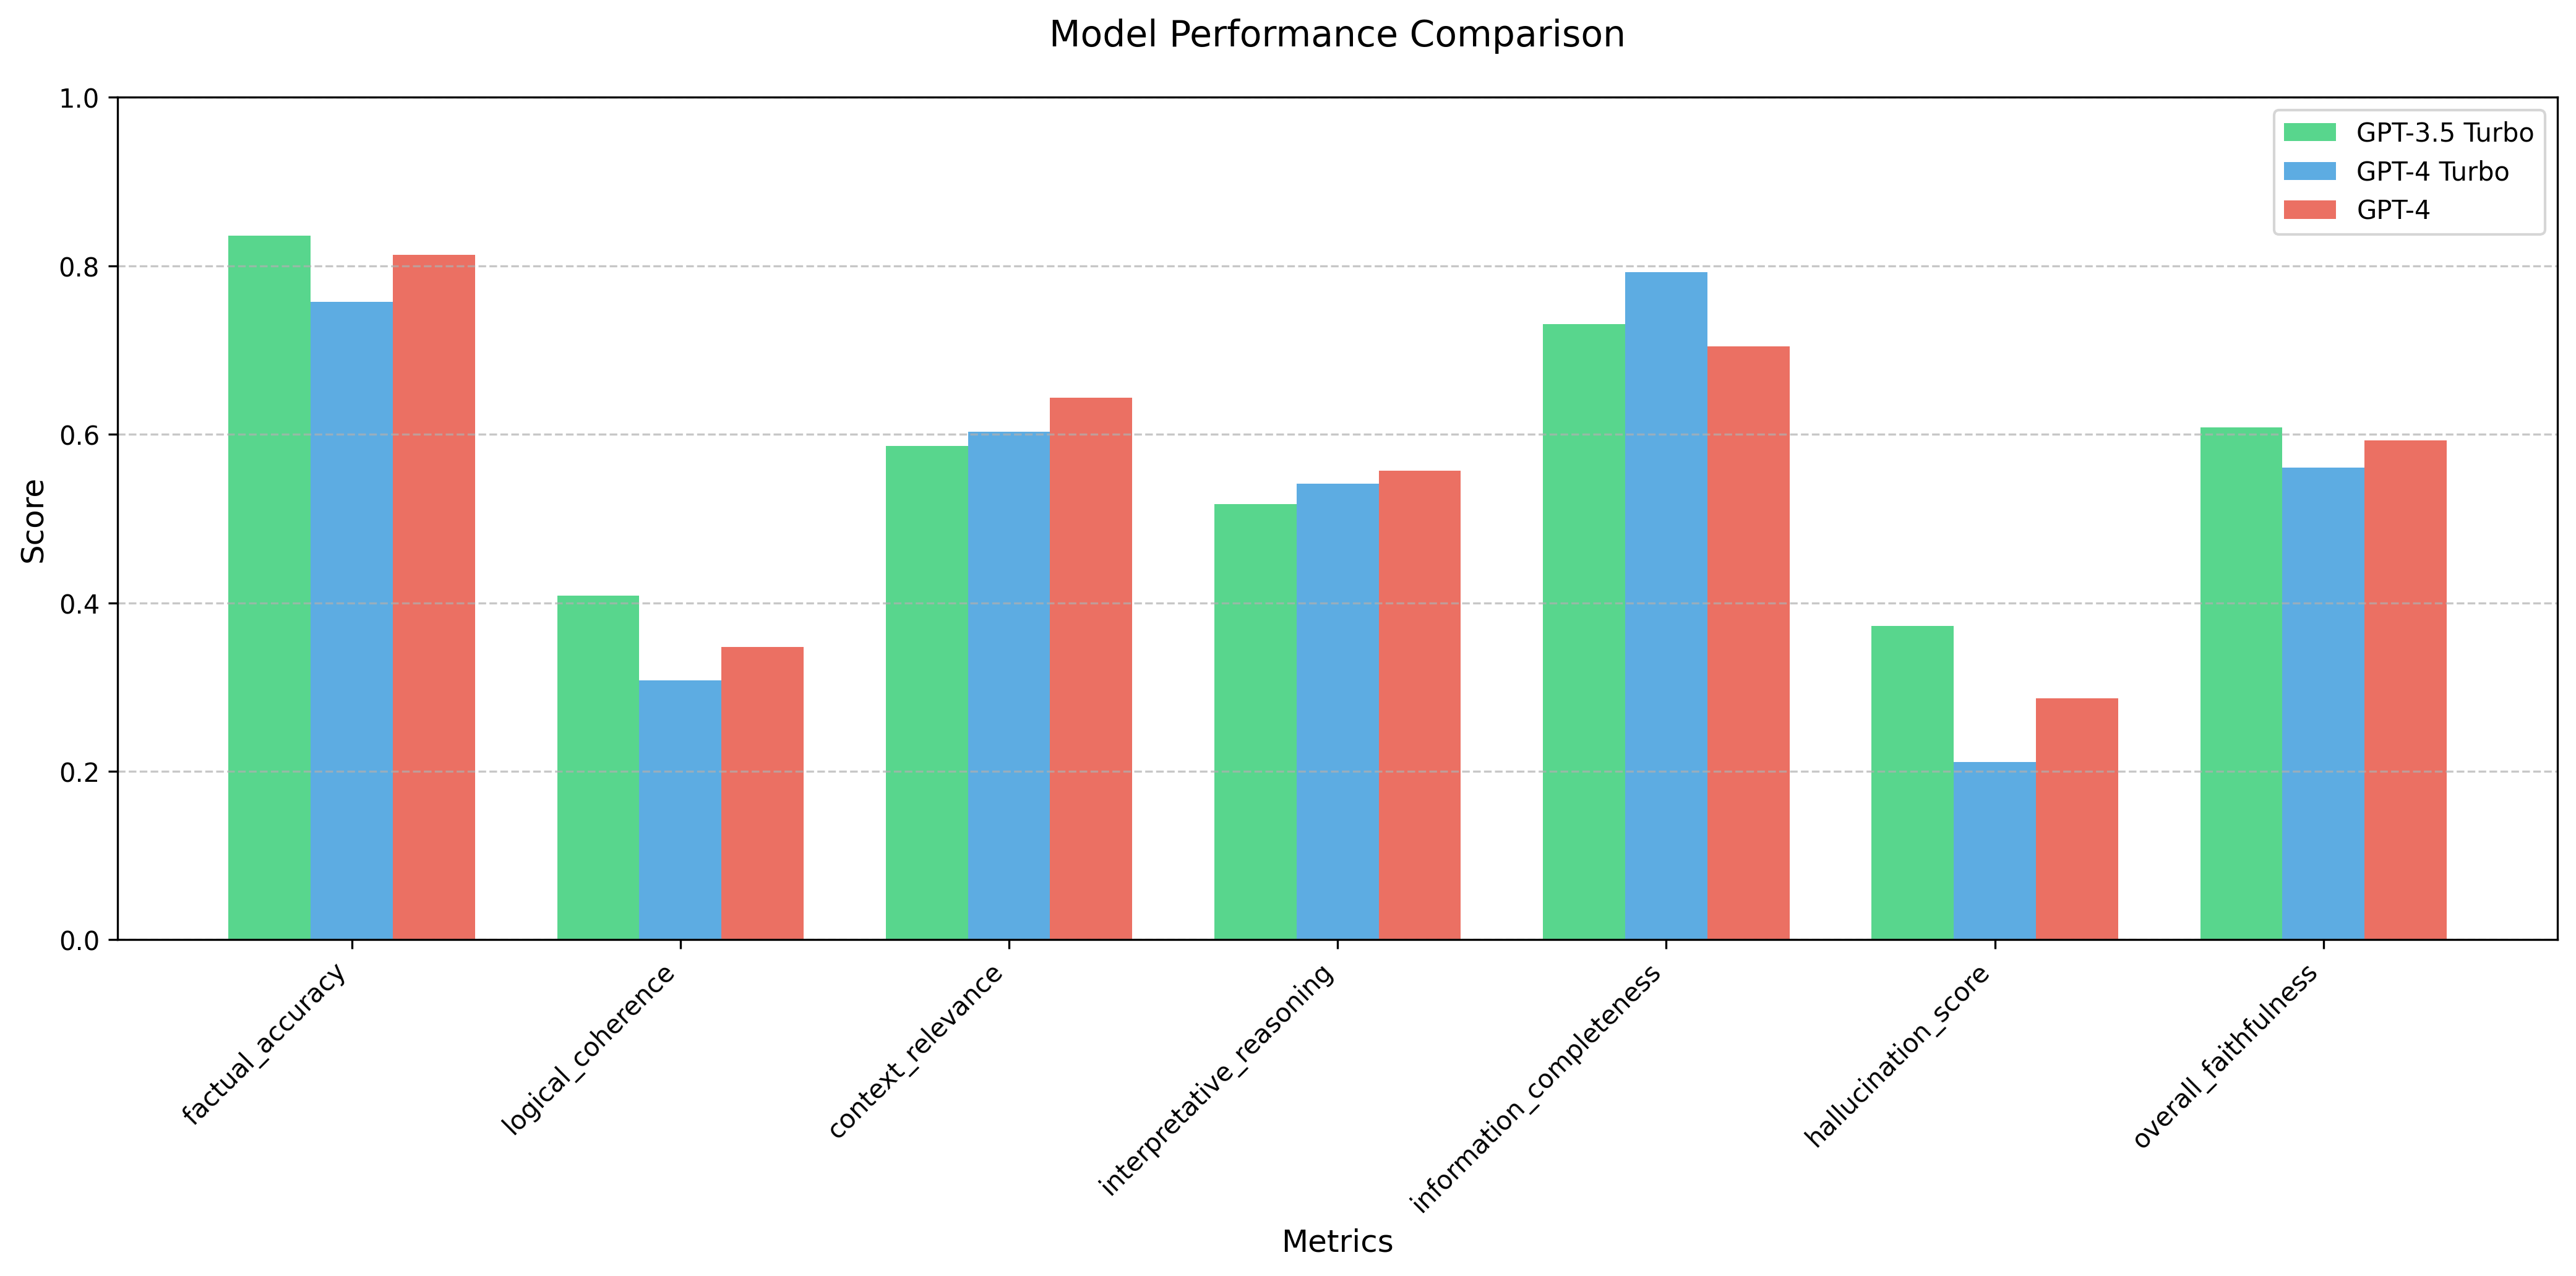
\includegraphics[width=0.8\textwidth]{figures/overall/model_comparison.png}
\caption{Comparative Performance Across Models}
\label{fig:model_comparison}
\end{figure}

\vspace{0.5em}
The model comparison reveals several interesting patterns:
\begin{itemize}
    \item Factual accuracy remains consistently high across all models (>0.75)
    \item Logical coherence shows the most variation between models
    \item Information completeness demonstrates an inverse relationship with hallucination scores
\end{itemize}

\vspace{0.5em}
\subsubsection{Overall Metrics Radar Charts}
The radar charts in Figure~\ref{fig:overall_metrics_radar} provide a multidimensional view of each model's performance, highlighting their unique characteristics and balance across different metrics.

\begin{figure}[!htbp]
\centering
\begin{subfigure}[b]{0.32\textwidth}
    \centering
    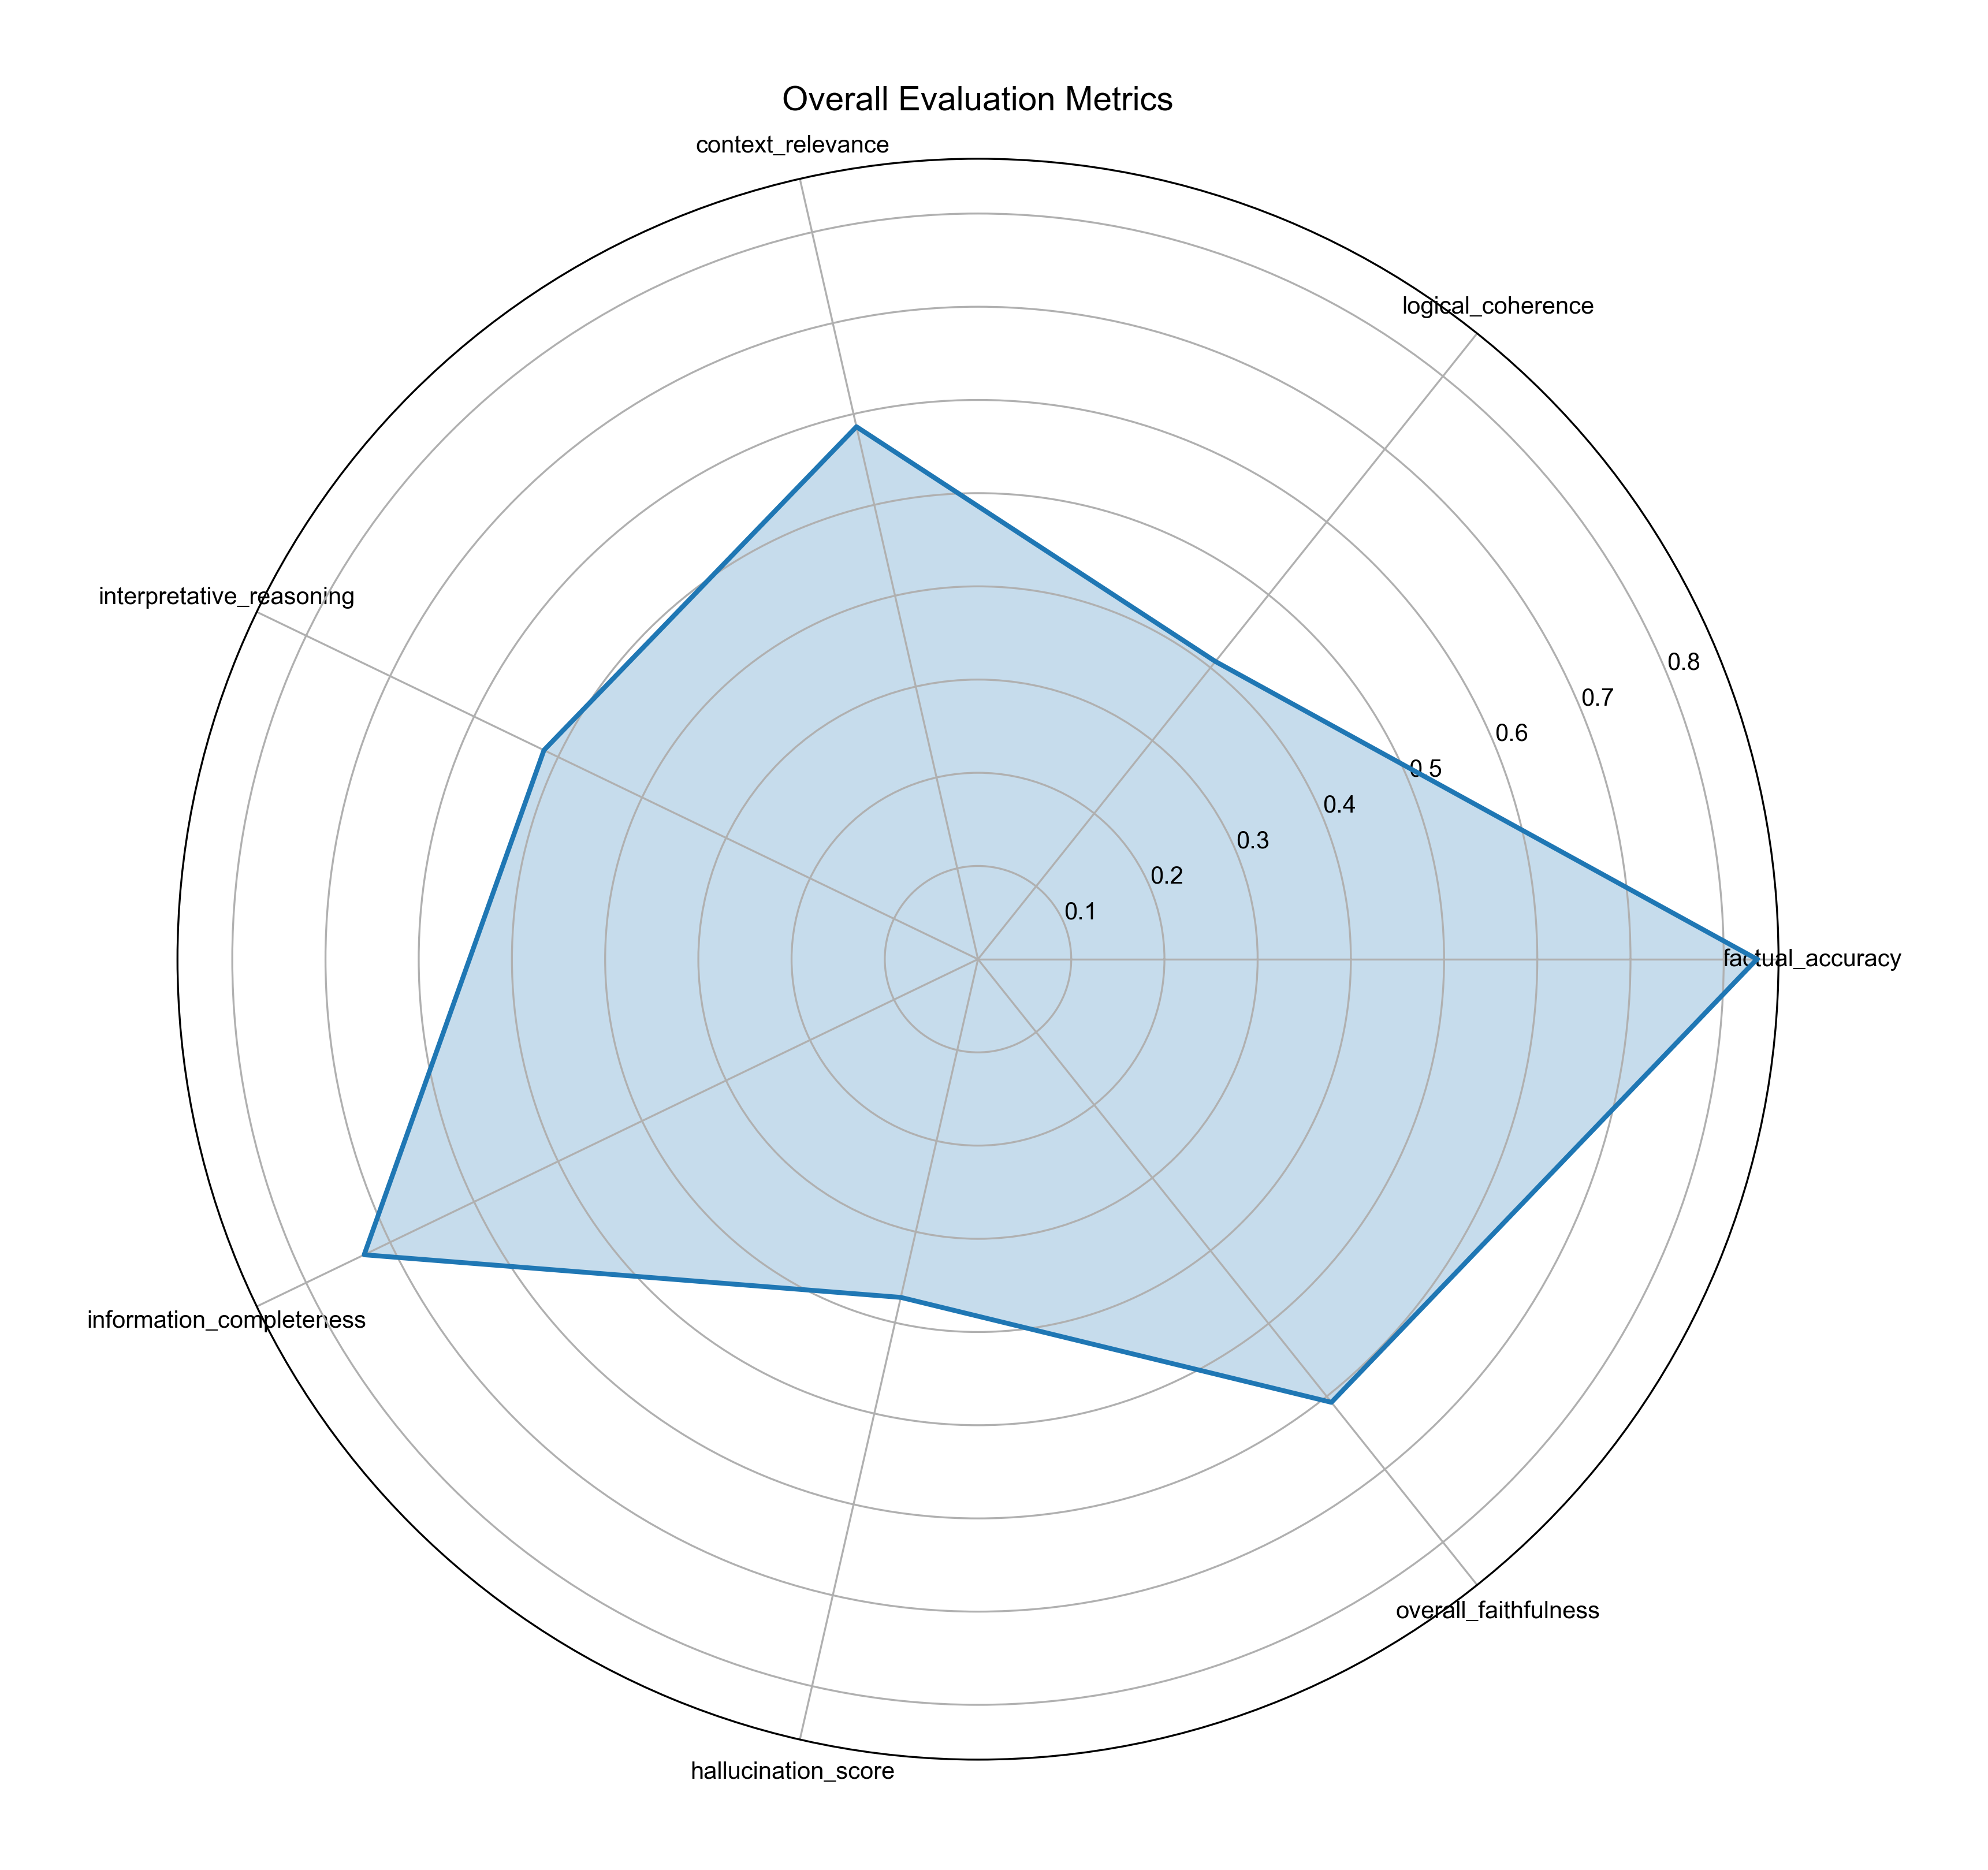
\includegraphics[width=\textwidth]{figures/overall/overall_metrics_radar_gpt-3.5-turbo.png}
    \caption{GPT-3.5-Turbo Metrics}
    \label{fig:overall_metrics_radar_gpt35}
\end{subfigure}
\hfill
\begin{subfigure}[b]{0.32\textwidth}
    \centering
    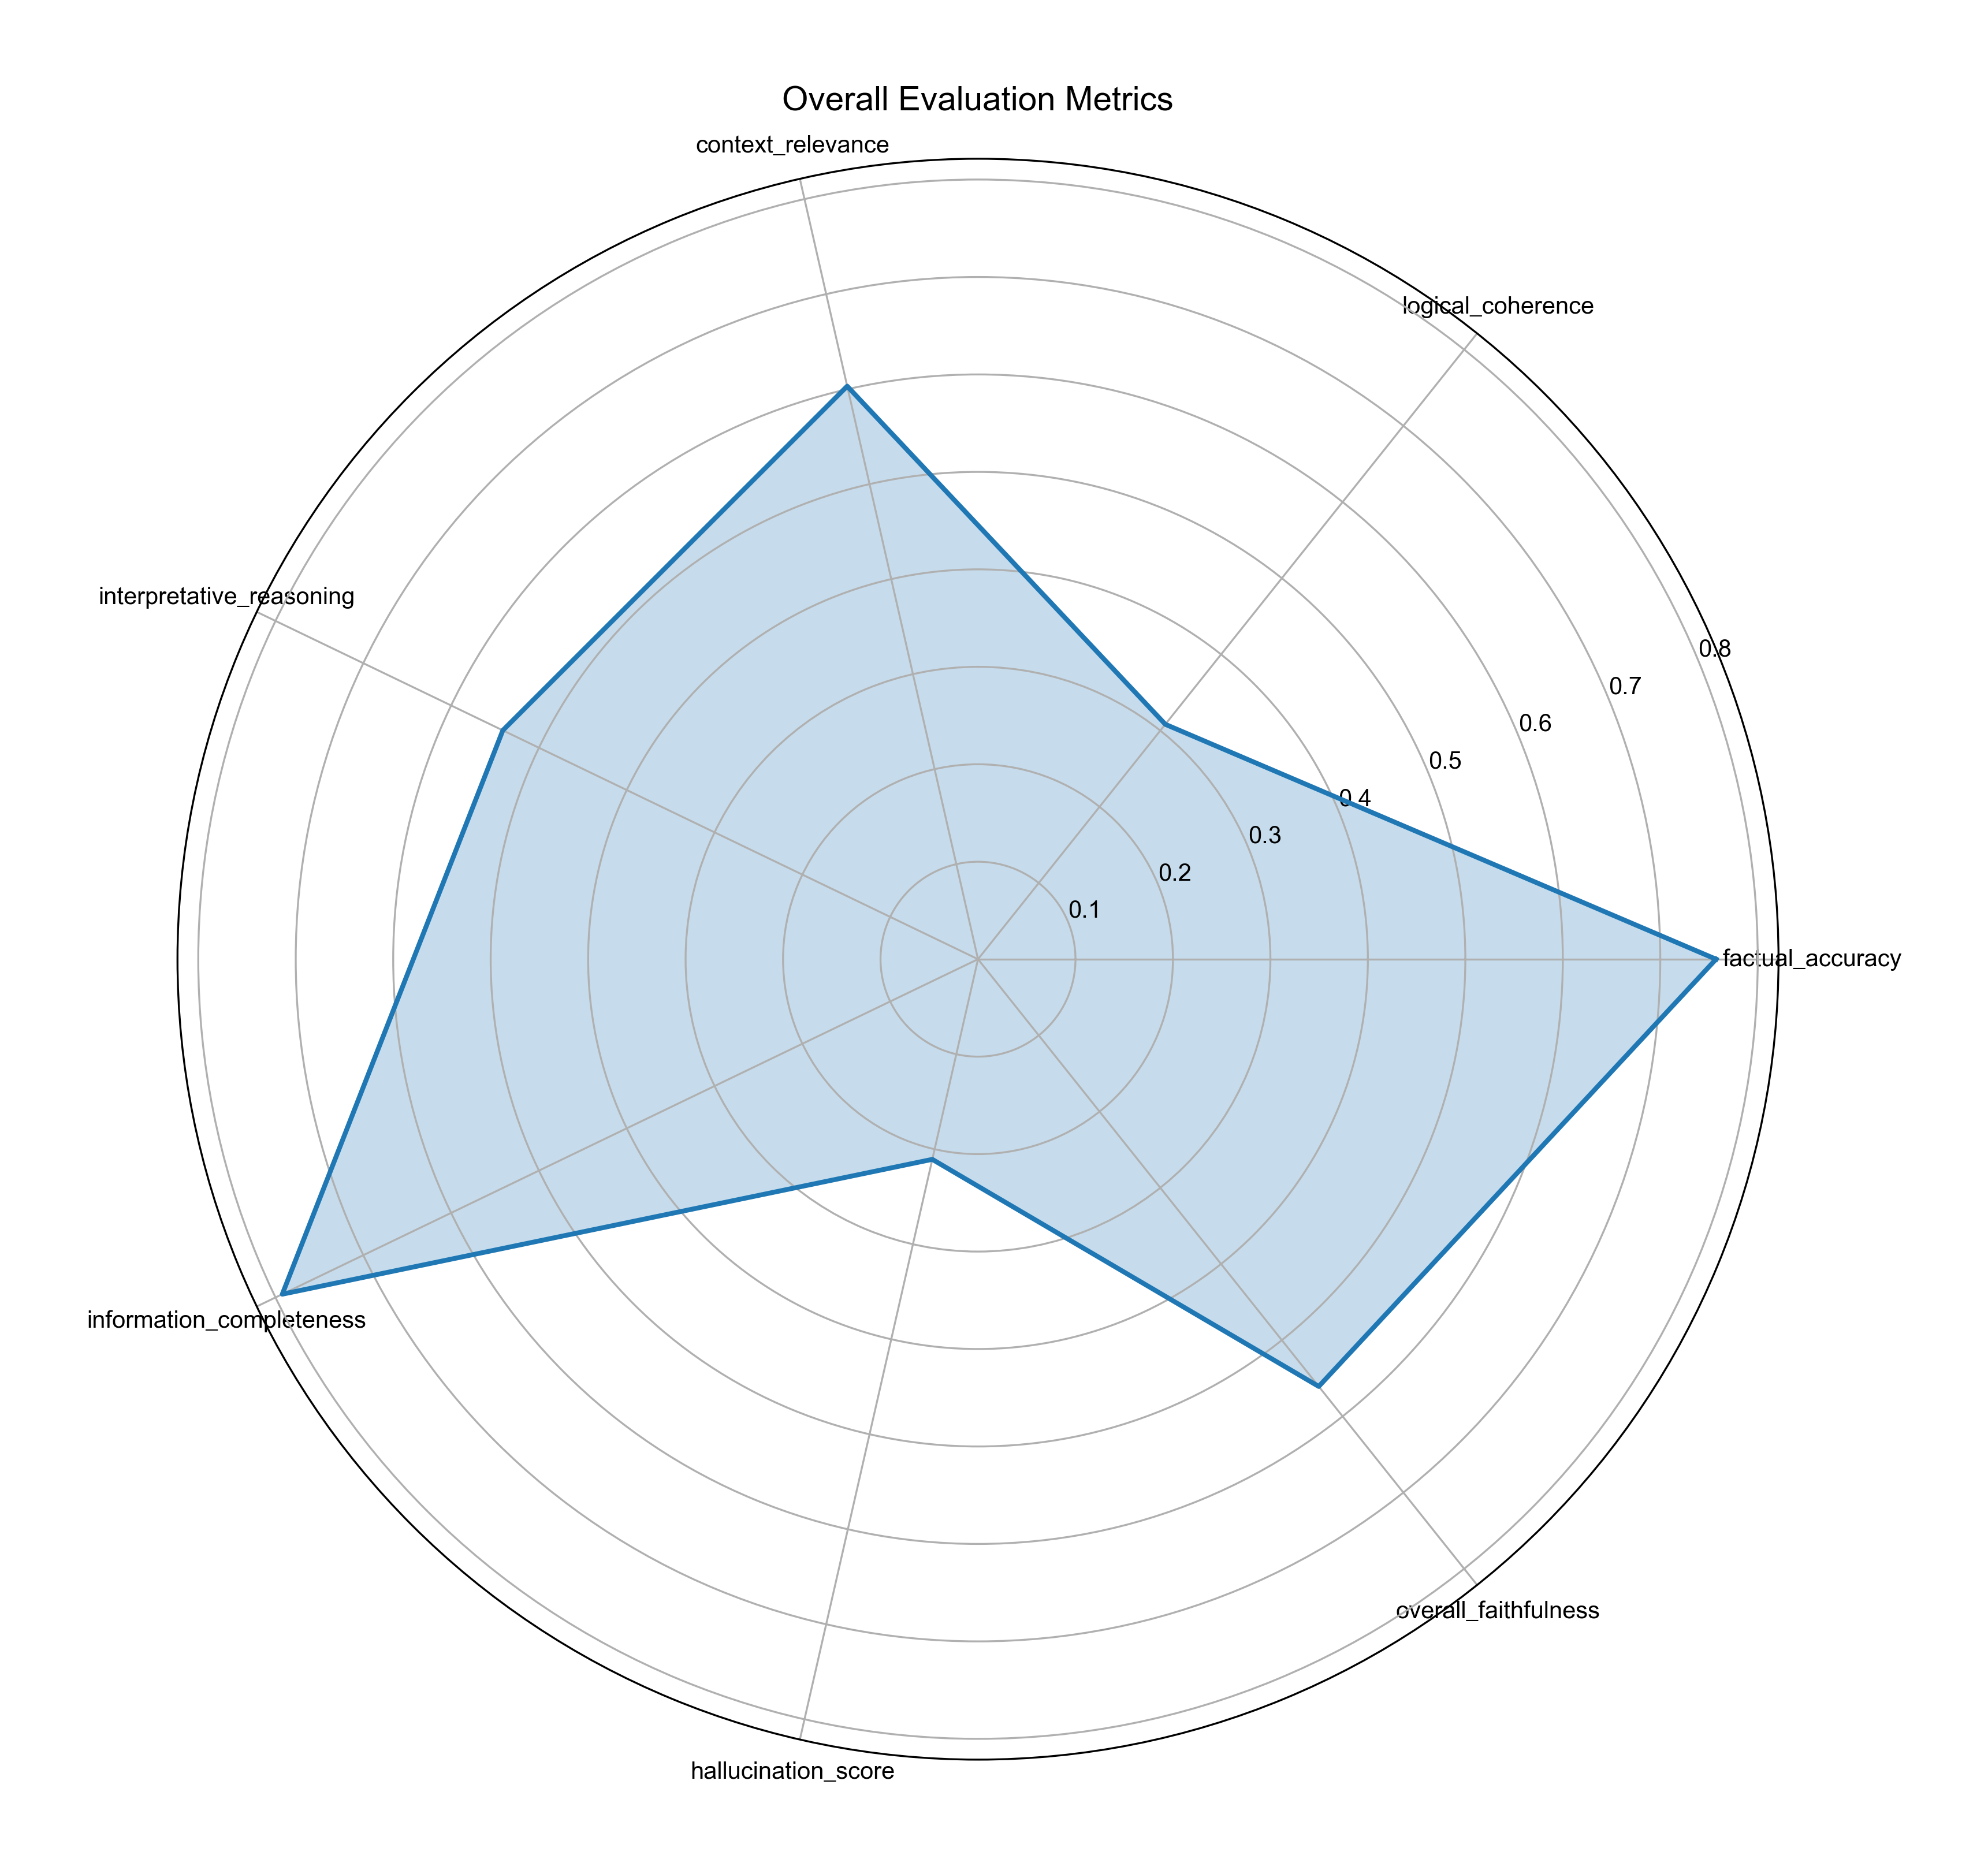
\includegraphics[width=\textwidth]{figures/overall/overall_metrics_radar_gpt-4-turbo.png}
    \caption{GPT-4-Turbo Metrics}
    \label{fig:overall_metrics_radar_gpt4t}
\end{subfigure}
\hfill
\begin{subfigure}[b]{0.32\textwidth}
    \centering
    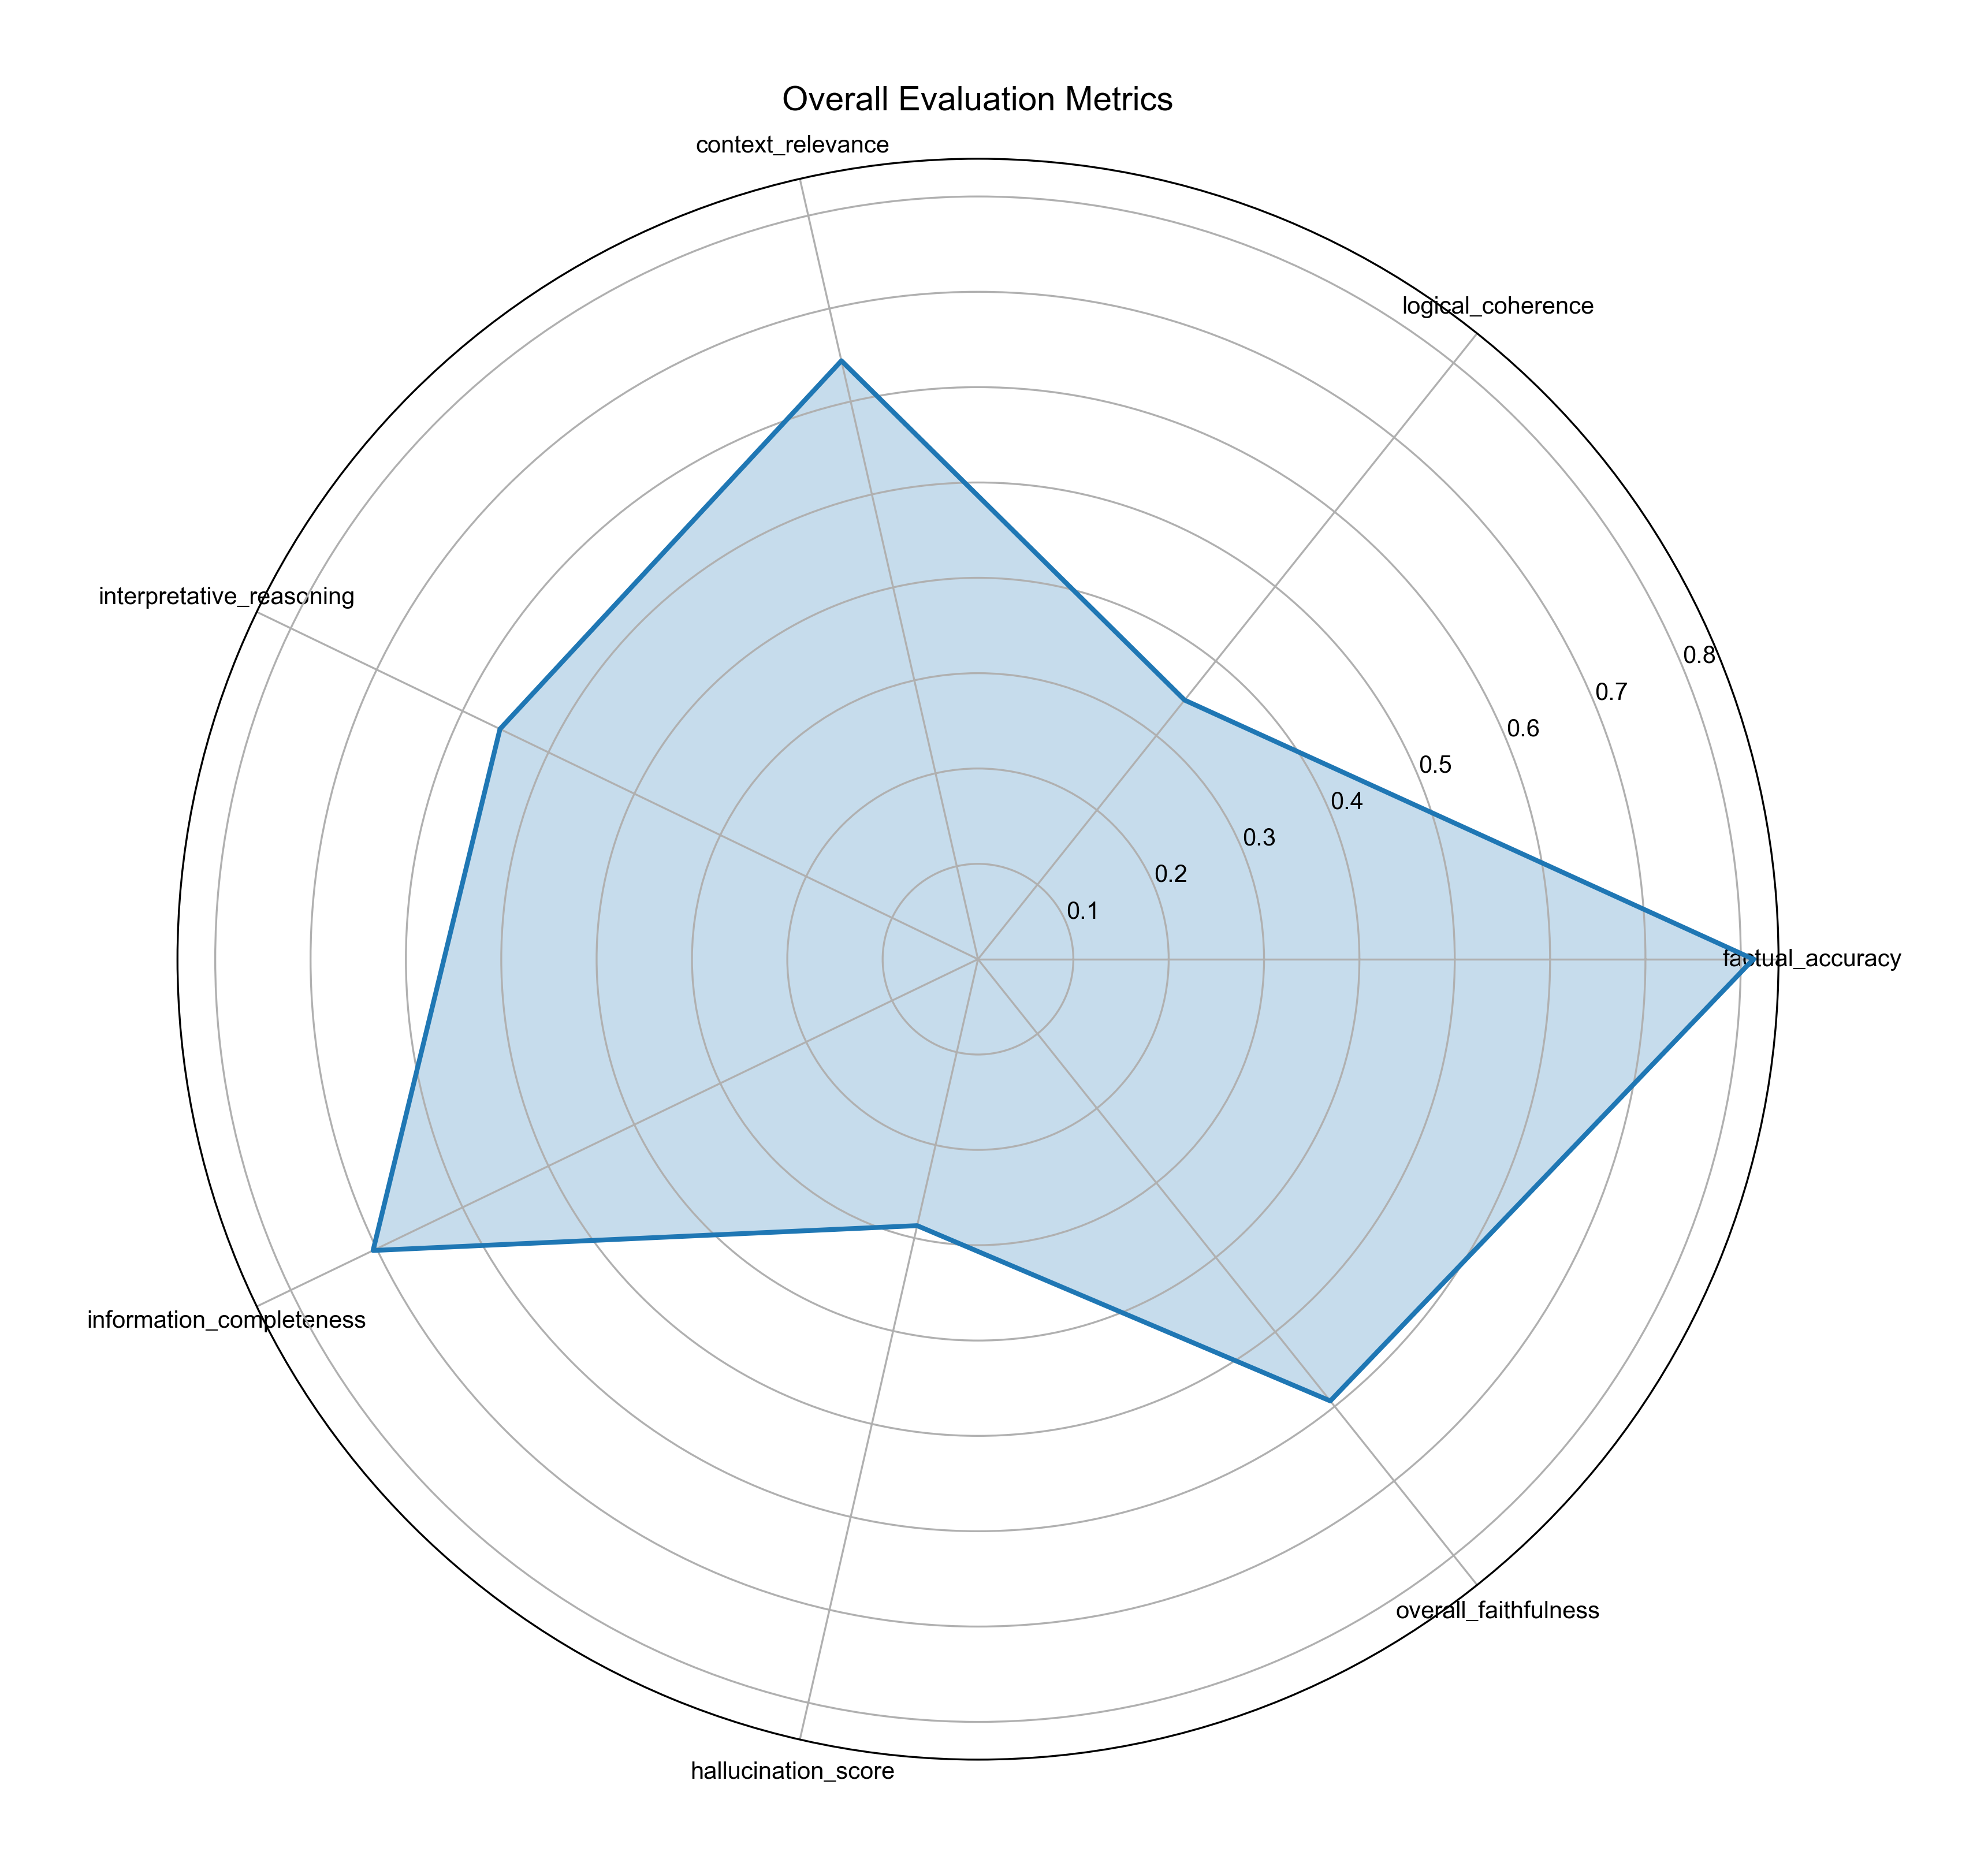
\includegraphics[width=\textwidth]{figures/overall/overall_metrics_radar_gpt-4.png}
    \caption{GPT-4 Metrics}
    \label{fig:overall_metrics_radar_gpt4}
\end{subfigure}
\caption{Overall Metrics Radar Charts by Model}
\label{fig:overall_metrics_radar}
\end{figure}

\textbf{Radar Chart Analysis}:
\begin{itemize}
    \item Each model exhibits distinct patterns in their metric distribution
    \item GPT-3.5-Turbo shows more balanced performance across metrics
    \item GPT-4 variants demonstrate stronger performance in specific areas
\end{itemize}

\subsubsection{Metrics Trend Analysis}
Building on our methodology described in Section~\ref{sec:methodology}, we analyzed the evolution of different metrics across various evaluation scenarios for each model, providing insights into their performance stability and patterns.

\begin{figure}[!htbp]
\centering
\begin{subfigure}{0.3\textwidth}
    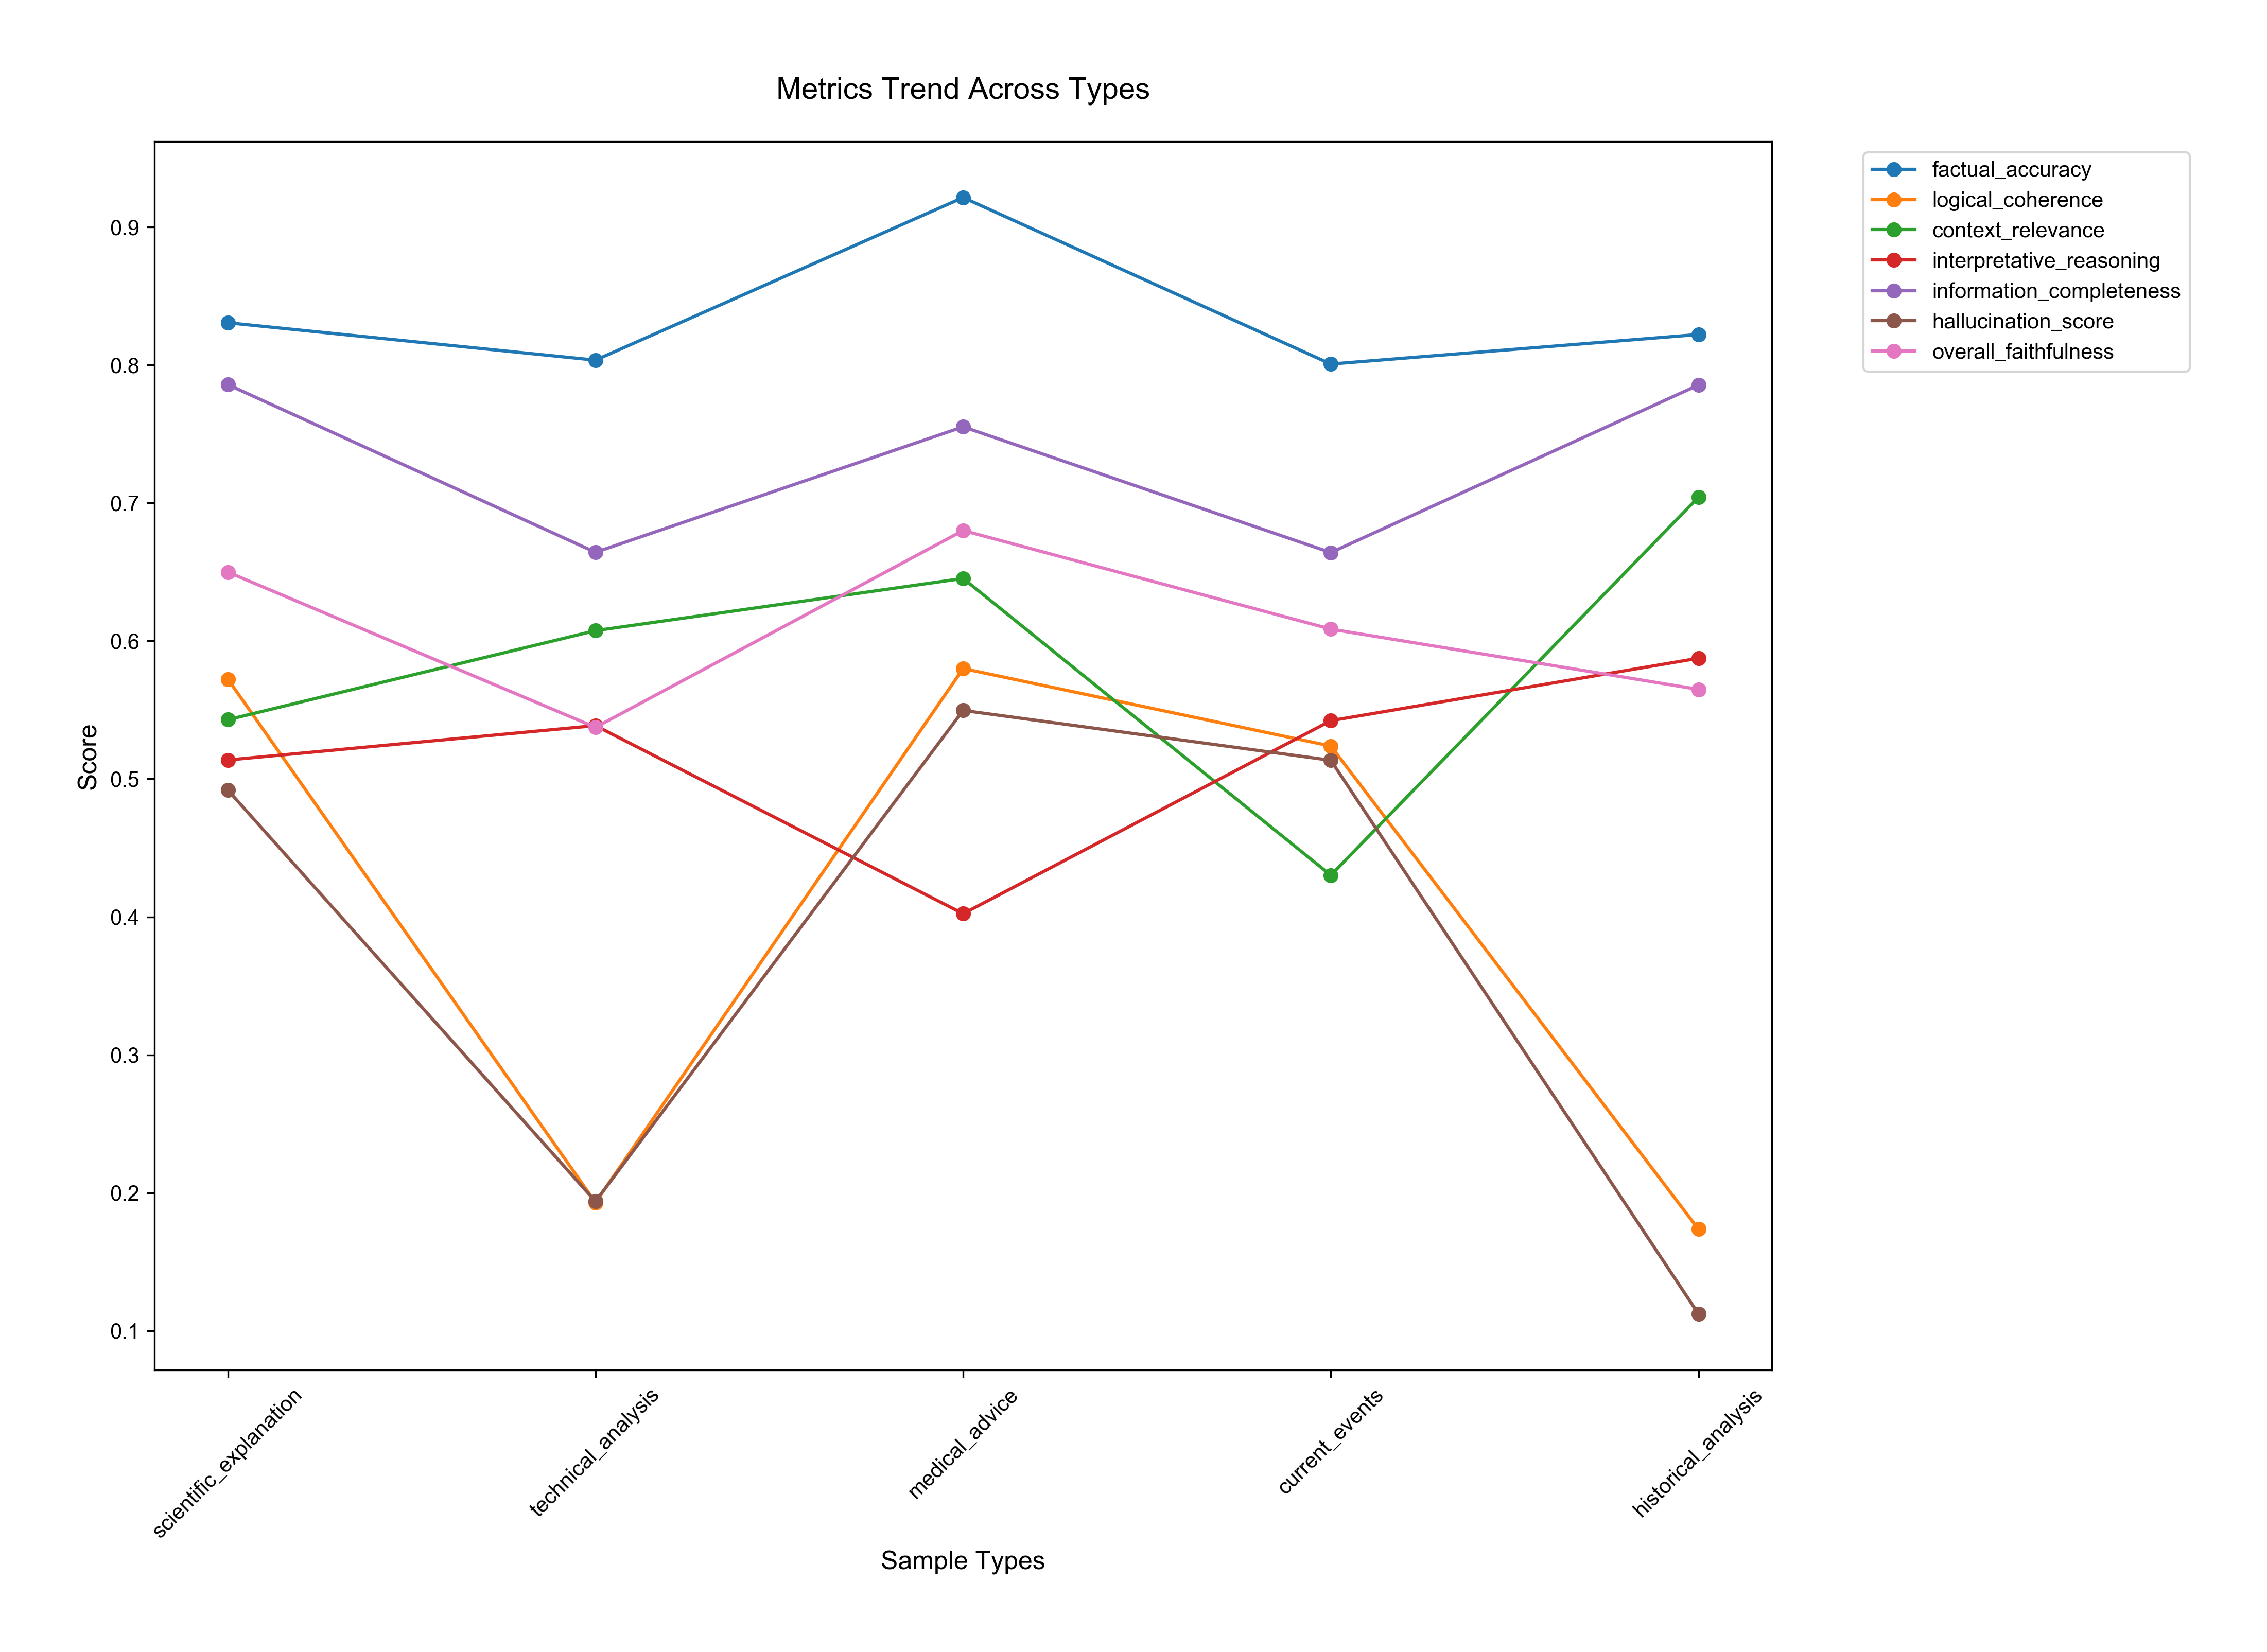
\includegraphics[width=\textwidth]{figures/overall/metrics_trend_gpt-3.5-turbo.png}
    \caption{GPT-3.5-Turbo Trends}
    \label{fig:metrics_trend_gpt35}
\end{subfigure}
\begin{subfigure}{0.3\textwidth}
    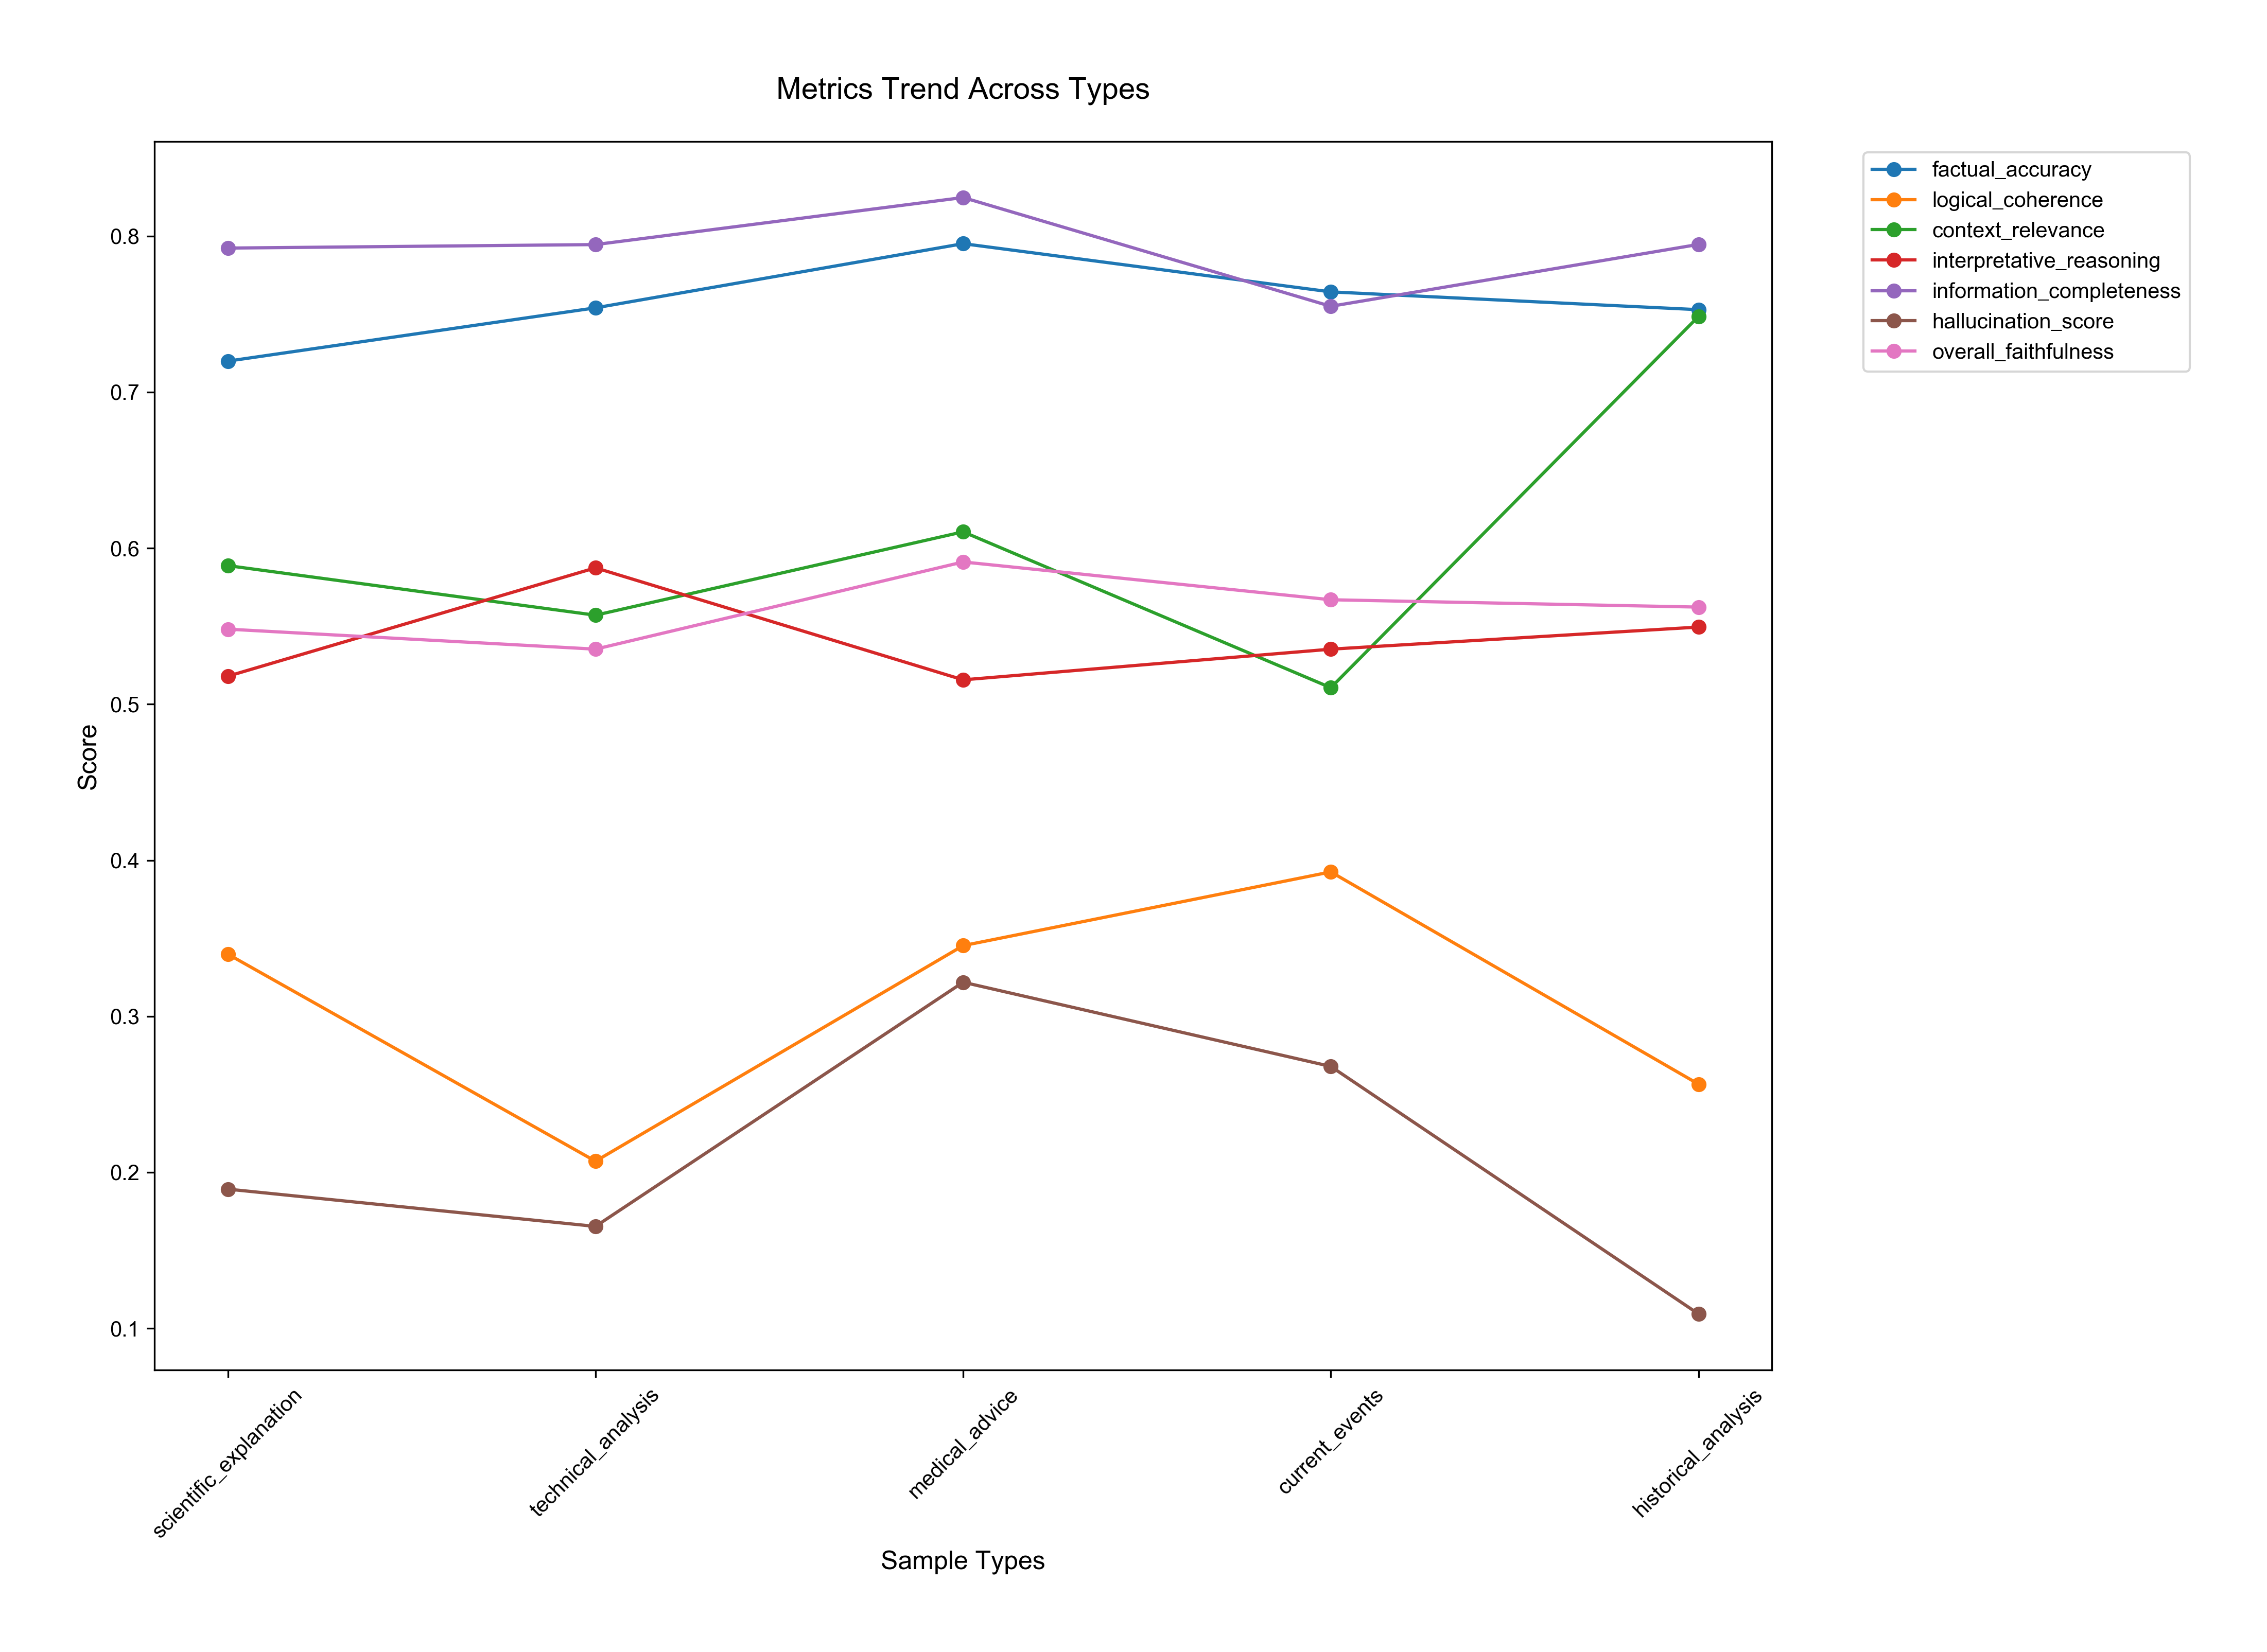
\includegraphics[width=\textwidth]{figures/overall/metrics_trend_gpt-4-turbo.png}
    \caption{GPT-4-Turbo Trends}
    \label{fig:metrics_trend_gpt4t}
\end{subfigure}
\begin{subfigure}{0.3\textwidth}
    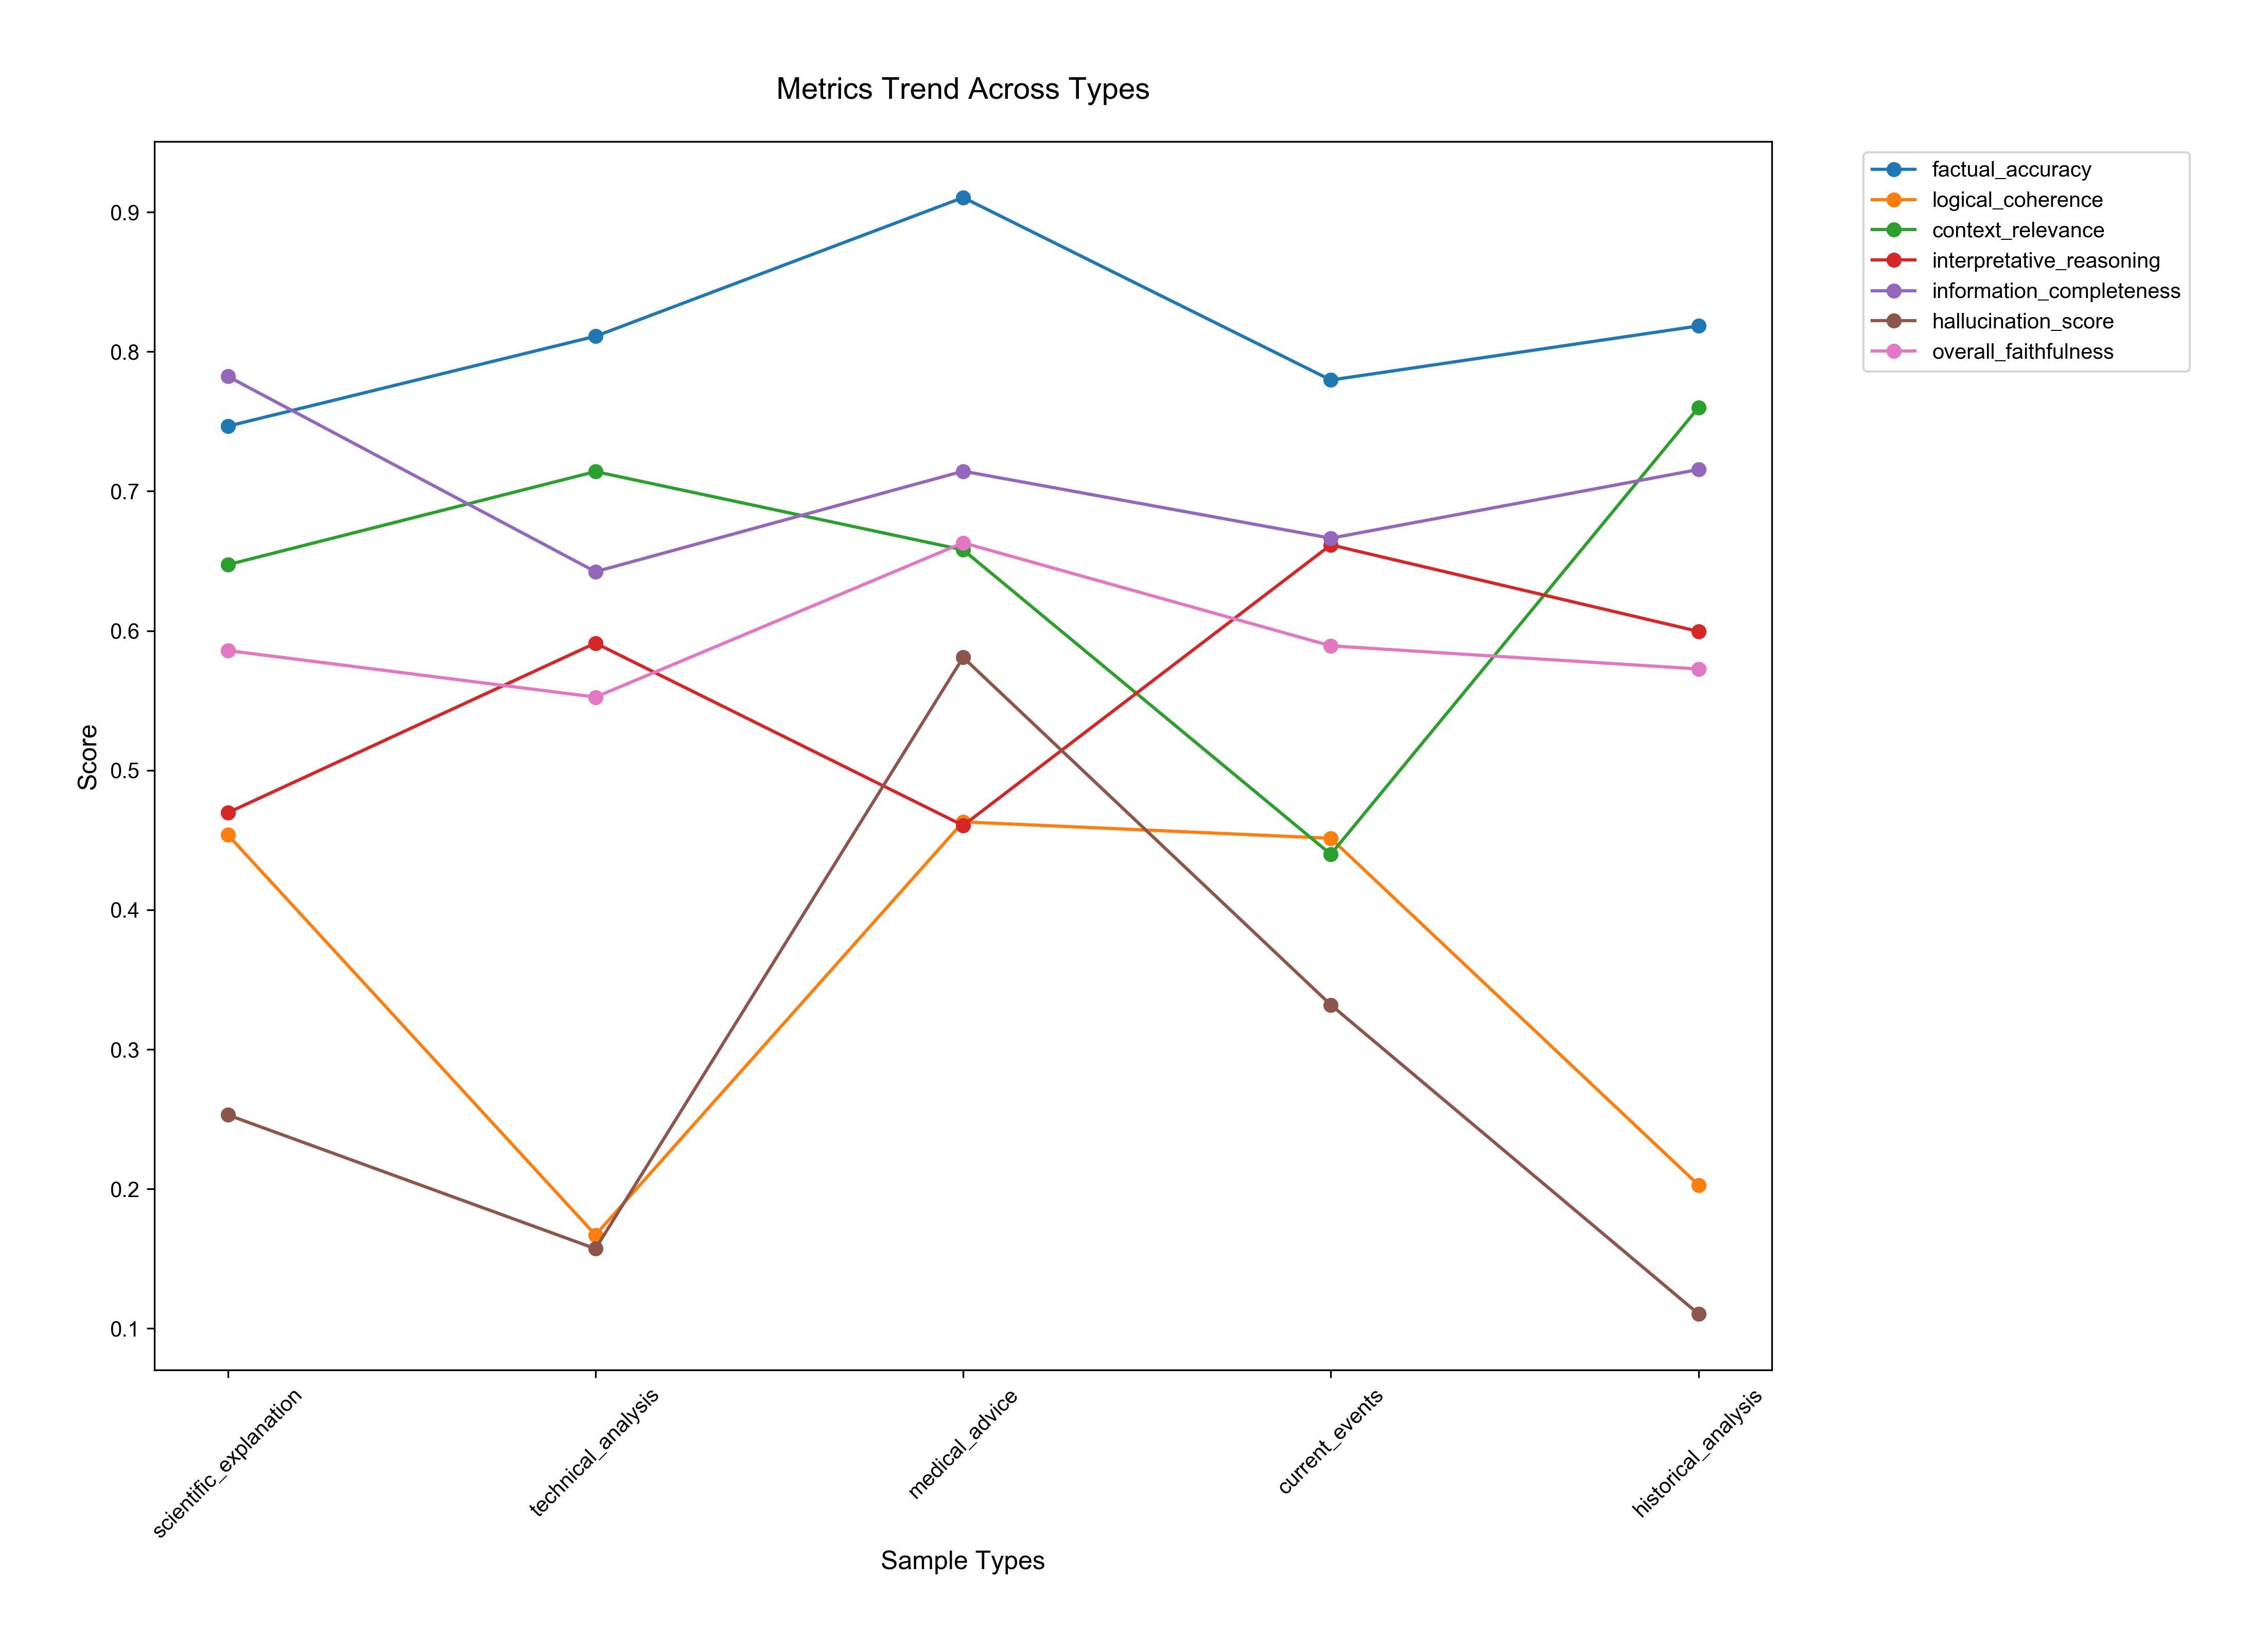
\includegraphics[width=\textwidth]{figures/overall/metrics_trend_gpt-4.png}
    \caption{GPT-4 Trends}
    \label{fig:metrics_trend_gpt4}
\end{subfigure}
\caption{Metrics Trend Analysis by Model}
\label{fig:metrics_trends}
\end{figure}

\textbf{Key Trend Observations}:
\begin{itemize}
    \item \textbf{Factual Accuracy}: Shows consistent high performance across all models, with minor fluctuations
    \item \textbf{Logical Coherence}: Exhibits the most variability, particularly in complex scenarios
    \item \textbf{Context Relevance}: Demonstrates steady improvement as models process more context
    \item \textbf{Hallucination Scores}: Show decreasing trends, indicating better control over fabricated information
\end{itemize}

\subsection{Type-Specific Evaluation Results}
Our analysis extends to different content types, revealing how models perform across various domains and contexts.

\subsubsection{Scientific Explanation}
The evaluation of scientific explanations focuses on the models' ability to accurately convey complex scientific concepts while maintaining factual integrity.

\begin{table}[!htbp]
\centering
\setlength{\tabcolsep}{4pt}  % Reduce table column spacing
\begin{tabular}{|l|c|c|c|c|c|c|c|}
\hline
\textbf{Model} & \textbf{FA} & \textbf{LC} & \textbf{CR} & \textbf{IR} 
& \textbf{IC} & \textbf{HS} & \textbf{OF} \\
\hline
GPT-3.5-Turbo & 0.83 & 0.57 & 0.54 & 0.51 & 0.79 & 0.49 & 0.65 \\
GPT-4-Turbo & 0.72 & 0.34 & 0.59 & 0.52 & 0.79 & 0.19 & 0.55 \\
GPT-4 & 0.75 & 0.45 & 0.65 & 0.47 & 0.78 & 0.25 & 0.59 \\
\hline
\end{tabular}
\caption{Scientific Explanation Metrics}
\label{tab:results_scientific_metrics}
\begin{flushleft}
\small
FA: Factual Accuracy, LC: Logical Coherence, CR: Context Relevance,\\
IR: Interpretative Reasoning, IC: Information Completeness, HS: Hallucination Score, OF: Overall Faithfulness
\end{flushleft}
\end{table}

\begin{figure}[!htbp]
\centering
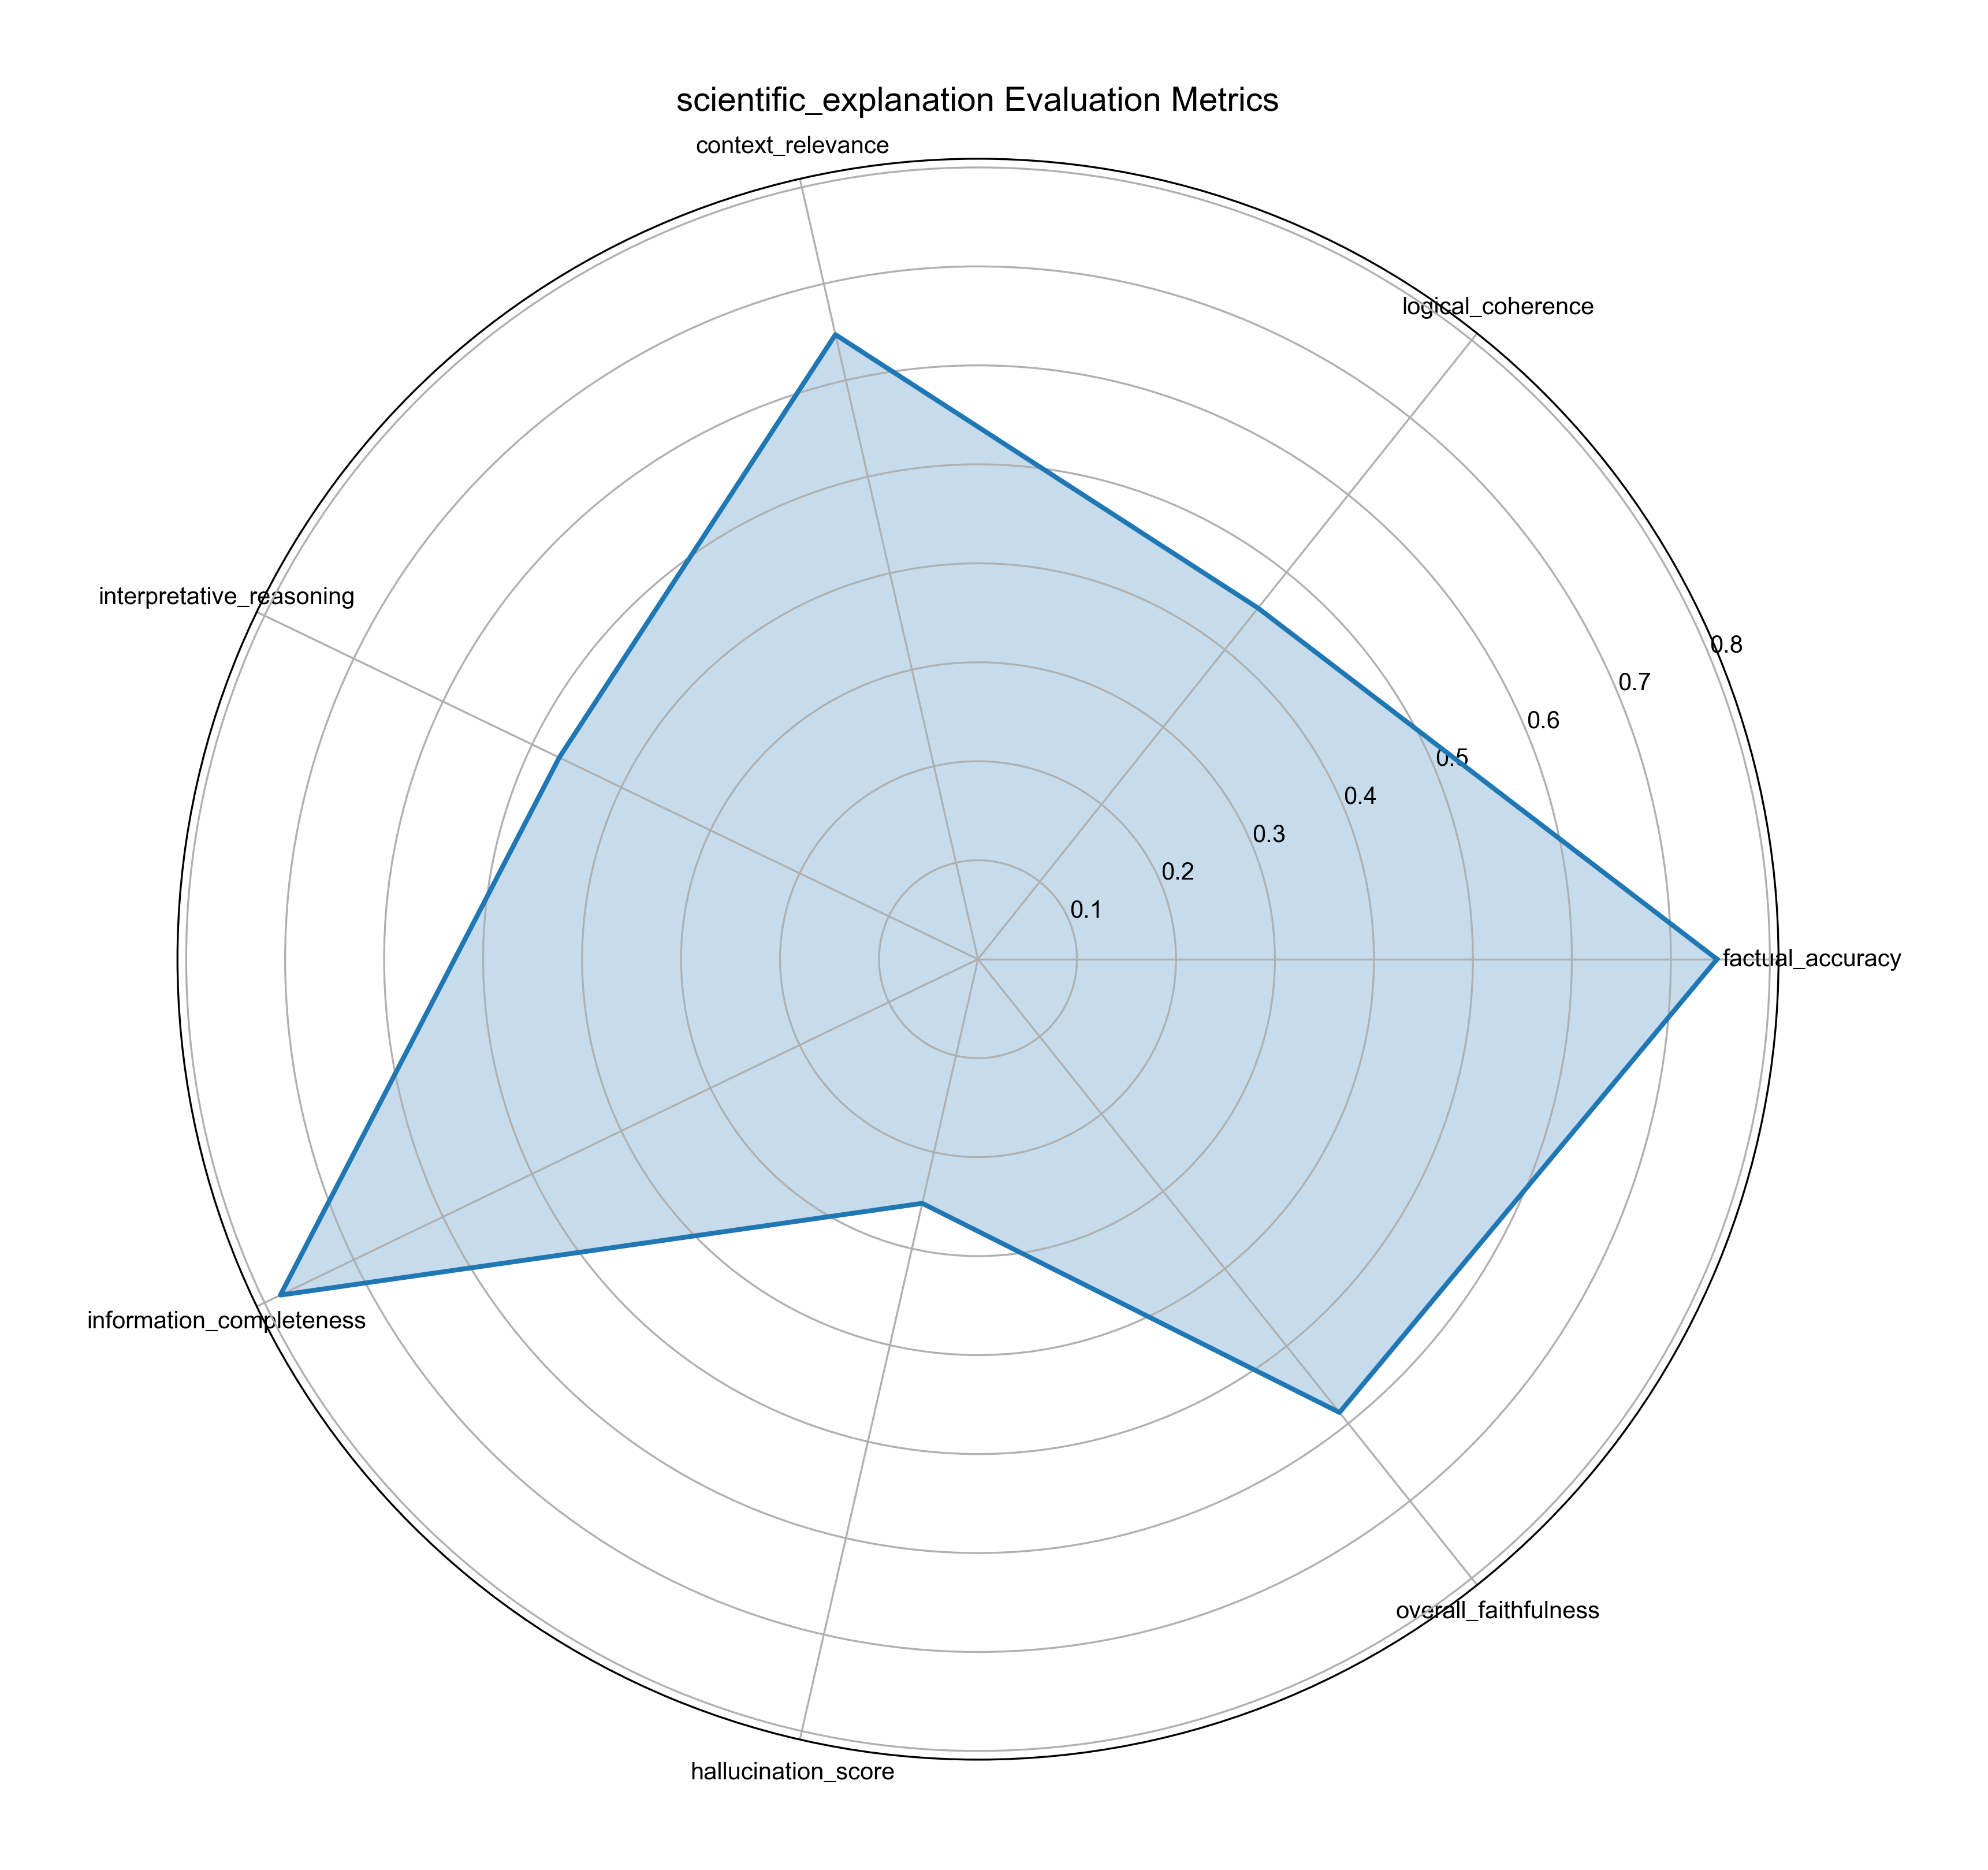
\includegraphics[width=0.6\textwidth]{figures/types/scientific_explanation_radar_gpt-4.png}
\caption{Scientific Explanation Performance Radar}
\label{fig:scientific_radar}
\end{figure}

\textbf{Analysis}:
\begin{itemize}
    \item GPT-3.5-Turbo demonstrates exceptional performance in scientific explanations, particularly in factual accuracy (0.83) and information completeness (0.79)
    \item Higher hallucination scores in this category suggest challenges in maintaining strict factual boundaries
    \item Logical coherence scores indicate room for improvement in structuring scientific arguments
\end{itemize}

\subsubsection{Technical Analysis}
For technical content, we evaluated the models' capability to handle detailed technical information and maintain accuracy in specialized contexts.

\begin{table}[!htbp]
\centering
\setlength{\tabcolsep}{4pt}  % Reduce table column spacing
\begin{tabular}{|l|c|c|c|c|c|c|c|}
\hline
\textbf{Model} & \textbf{FA} & \textbf{LC} & \textbf{CR} & \textbf{IR} 
& \textbf{IC} & \textbf{HS} & \textbf{OF} \\
\hline
GPT-3.5-Turbo & 0.80 & 0.19 & 0.61 & 0.54 & 0.66 & 0.19 & 0.54 \\
GPT-4-Turbo & 0.75 & 0.21 & 0.56 & 0.59 & 0.79 & 0.17 & 0.54 \\
GPT-4 & 0.81 & 0.17 & 0.71 & 0.59 & 0.64 & 0.16 & 0.55 \\
\hline
\end{tabular}
\caption{Technical Analysis Metrics}
\label{tab:results_technical_metrics}
\begin{flushleft}
\small
FA: Factual Accuracy, LC: Logical Coherence, CR: Context Relevance,\\
IR: Interpretative Reasoning, IC: Information Completeness, HS: Hallucination Score, OF: Overall Faithfulness
\end{flushleft}
\end{table}

\begin{figure}[!htbp]
\centering
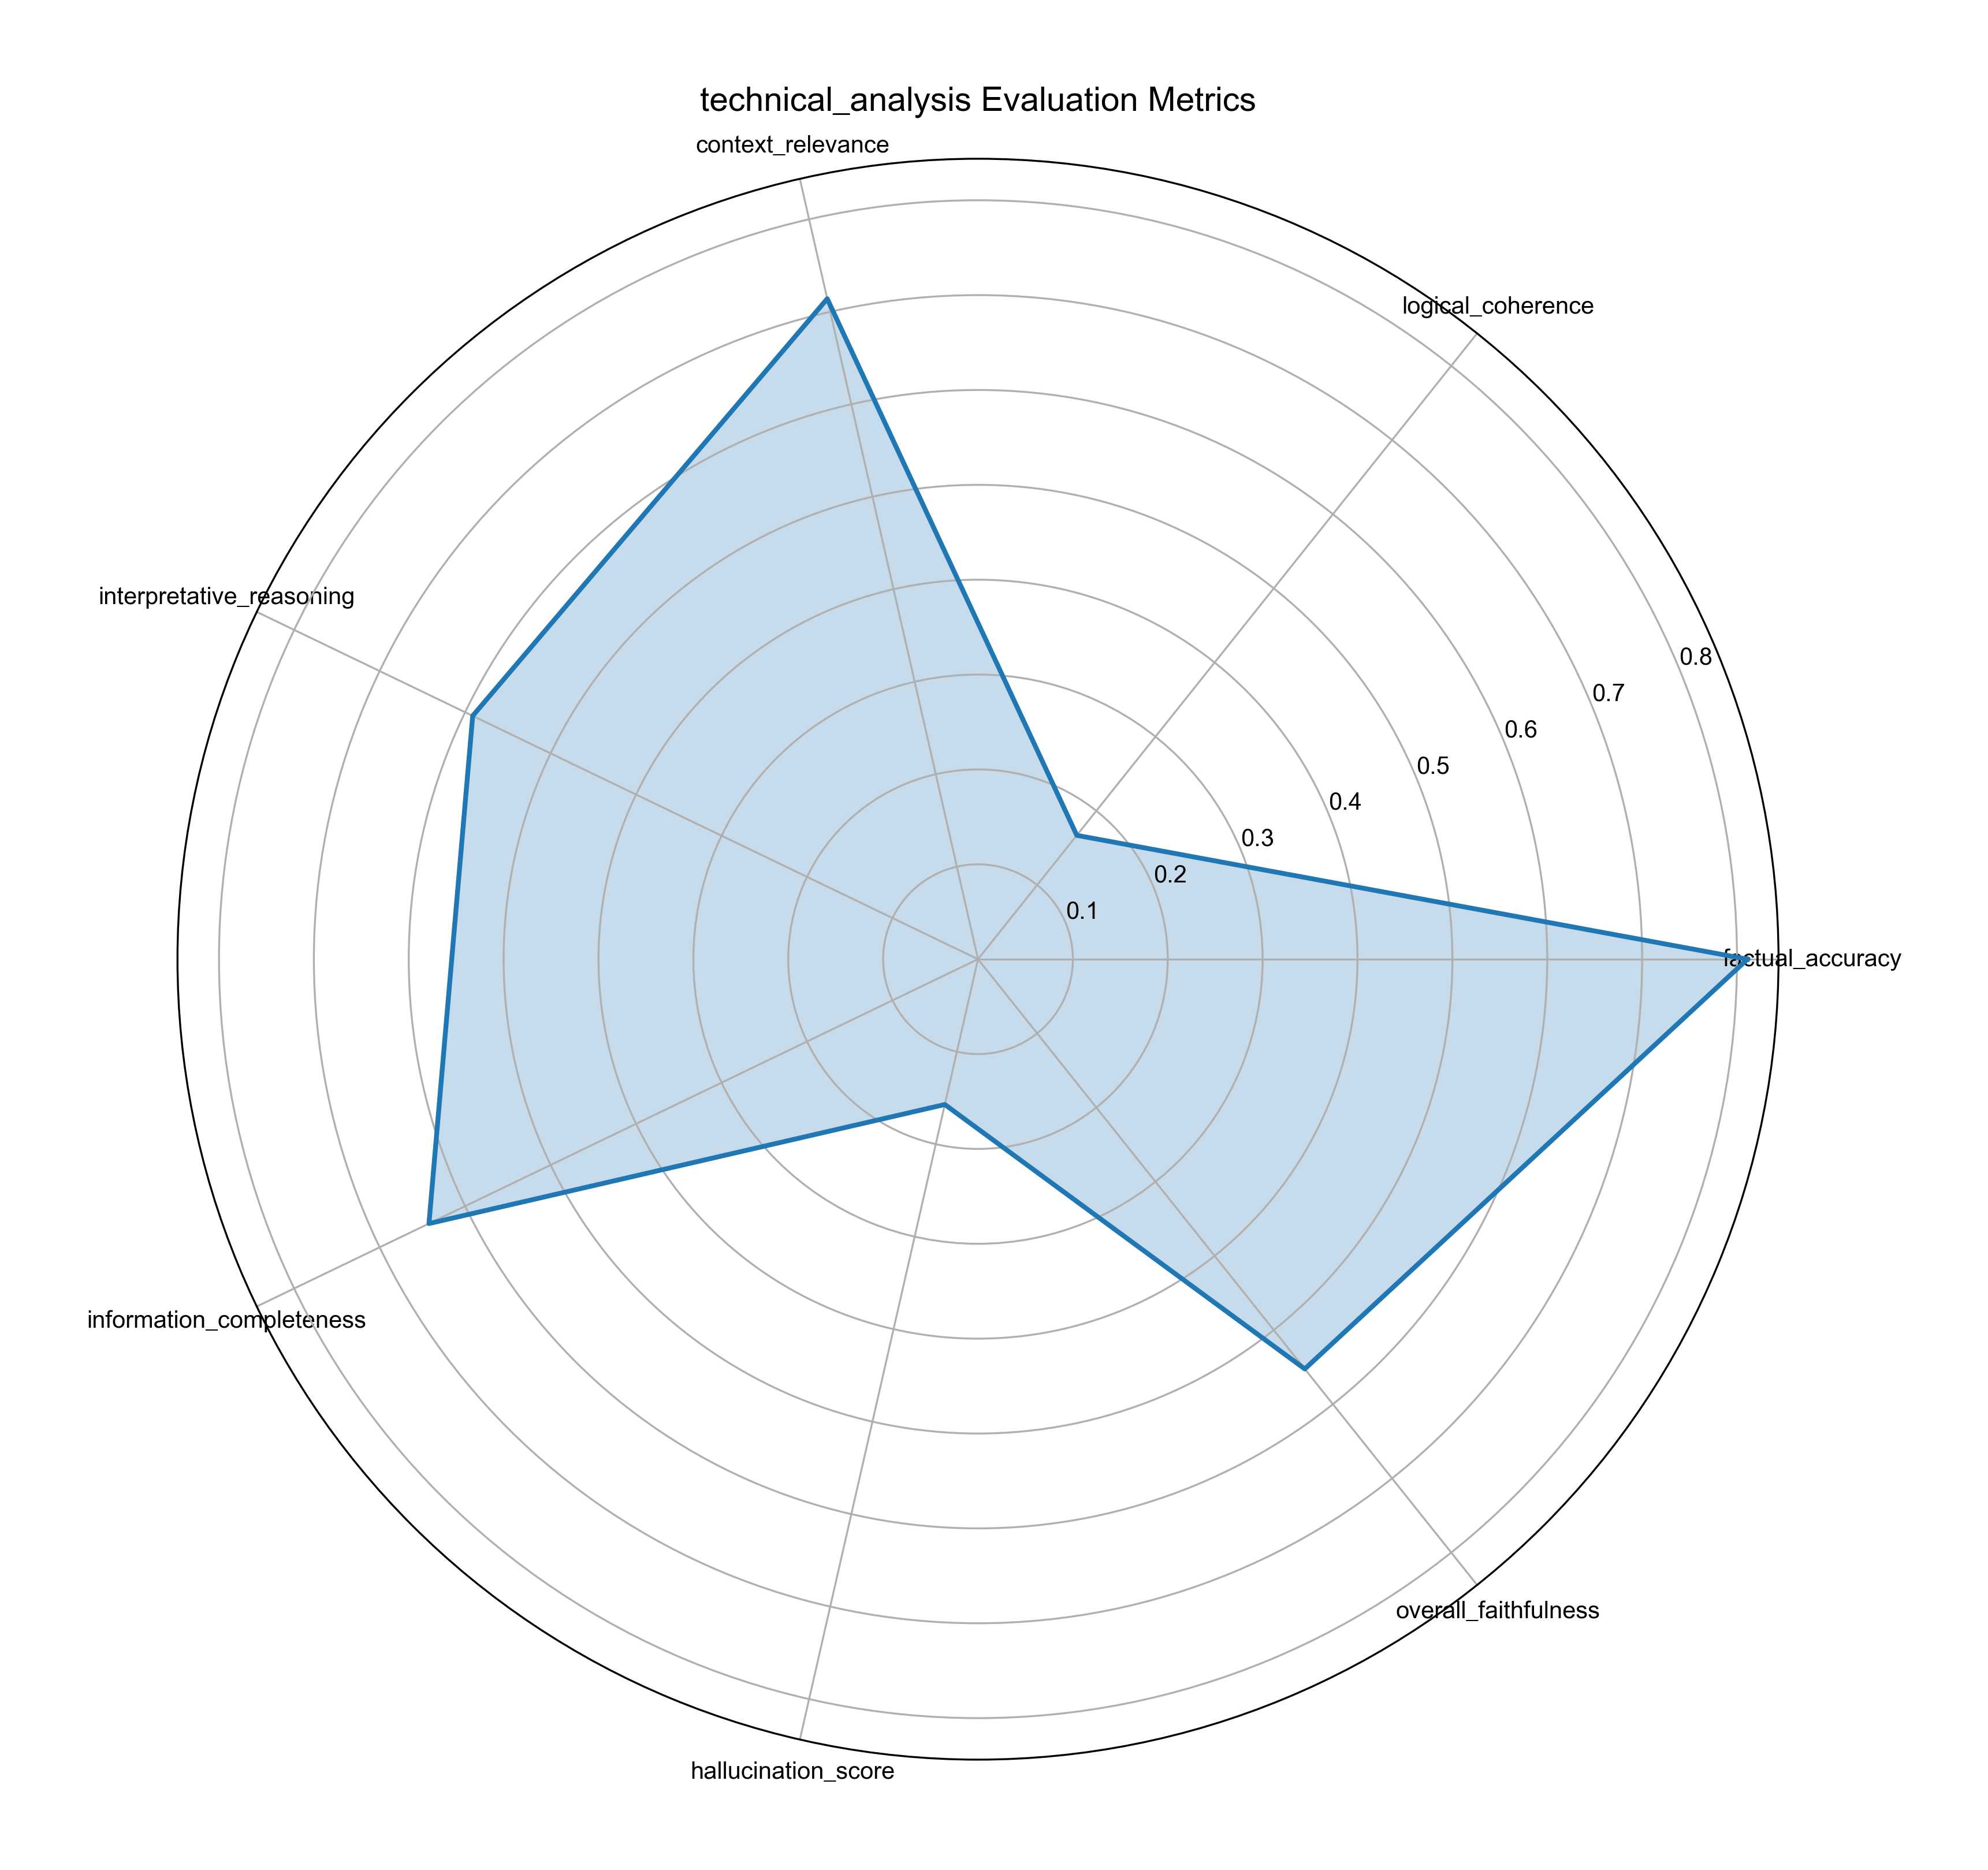
\includegraphics[width=0.6\textwidth]{figures/types/technical_analysis_radar_gpt-4.png}
\caption{Technical Analysis Performance Radar}
\label{fig:technical_radar}
\end{figure}

\textbf{Analysis}:
\begin{itemize}
    \item All models show improved performance in factual accuracy for technical content
    \item GPT-4 achieves the highest context relevance (0.7141), indicating better understanding of technical contexts
    \item Lower logical coherence scores suggest challenges in organizing technical information
\end{itemize}

\subsubsection{Medical Advice}
The medical advice evaluation assessed the models' ability to provide accurate and reliable health-related information.

\begin{table}[!htbp]
\centering
\setlength{\tabcolsep}{4pt}  % Reduce table column spacing
\begin{tabular}{|l|c|c|c|c|c|c|c|}
\hline
\textbf{Model} & \textbf{FA} & \textbf{LC} & \textbf{CR} & \textbf{IR} 
& \textbf{IC} & \textbf{HS} & \textbf{OF} \\
\hline
GPT-3.5-Turbo & 0.92 & 0.58 & 0.65 & 0.40 & 0.76 & 0.55 & 0.68 \\
GPT-4-Turbo & 0.80 & 0.35 & 0.61 & 0.52 & 0.82 & 0.32 & 0.66 \\
GPT-4 & 0.91 & 0.46 & 0.66 & 0.46 & 0.71 & 0.58 & 0.66 \\
\hline
\end{tabular}
\caption{Medical Advice Metrics}
\label{tab:results_medical_metrics}
\begin{flushleft}
\small
FA: Factual Accuracy, LC: Logical Coherence, CR: Context Relevance,\\
IR: Interpretative Reasoning, IC: Information Completeness, HS: Hallucination Score, OF: Overall Faithfulness
\end{flushleft}
\end{table}

\begin{figure}[!htbp]
\centering
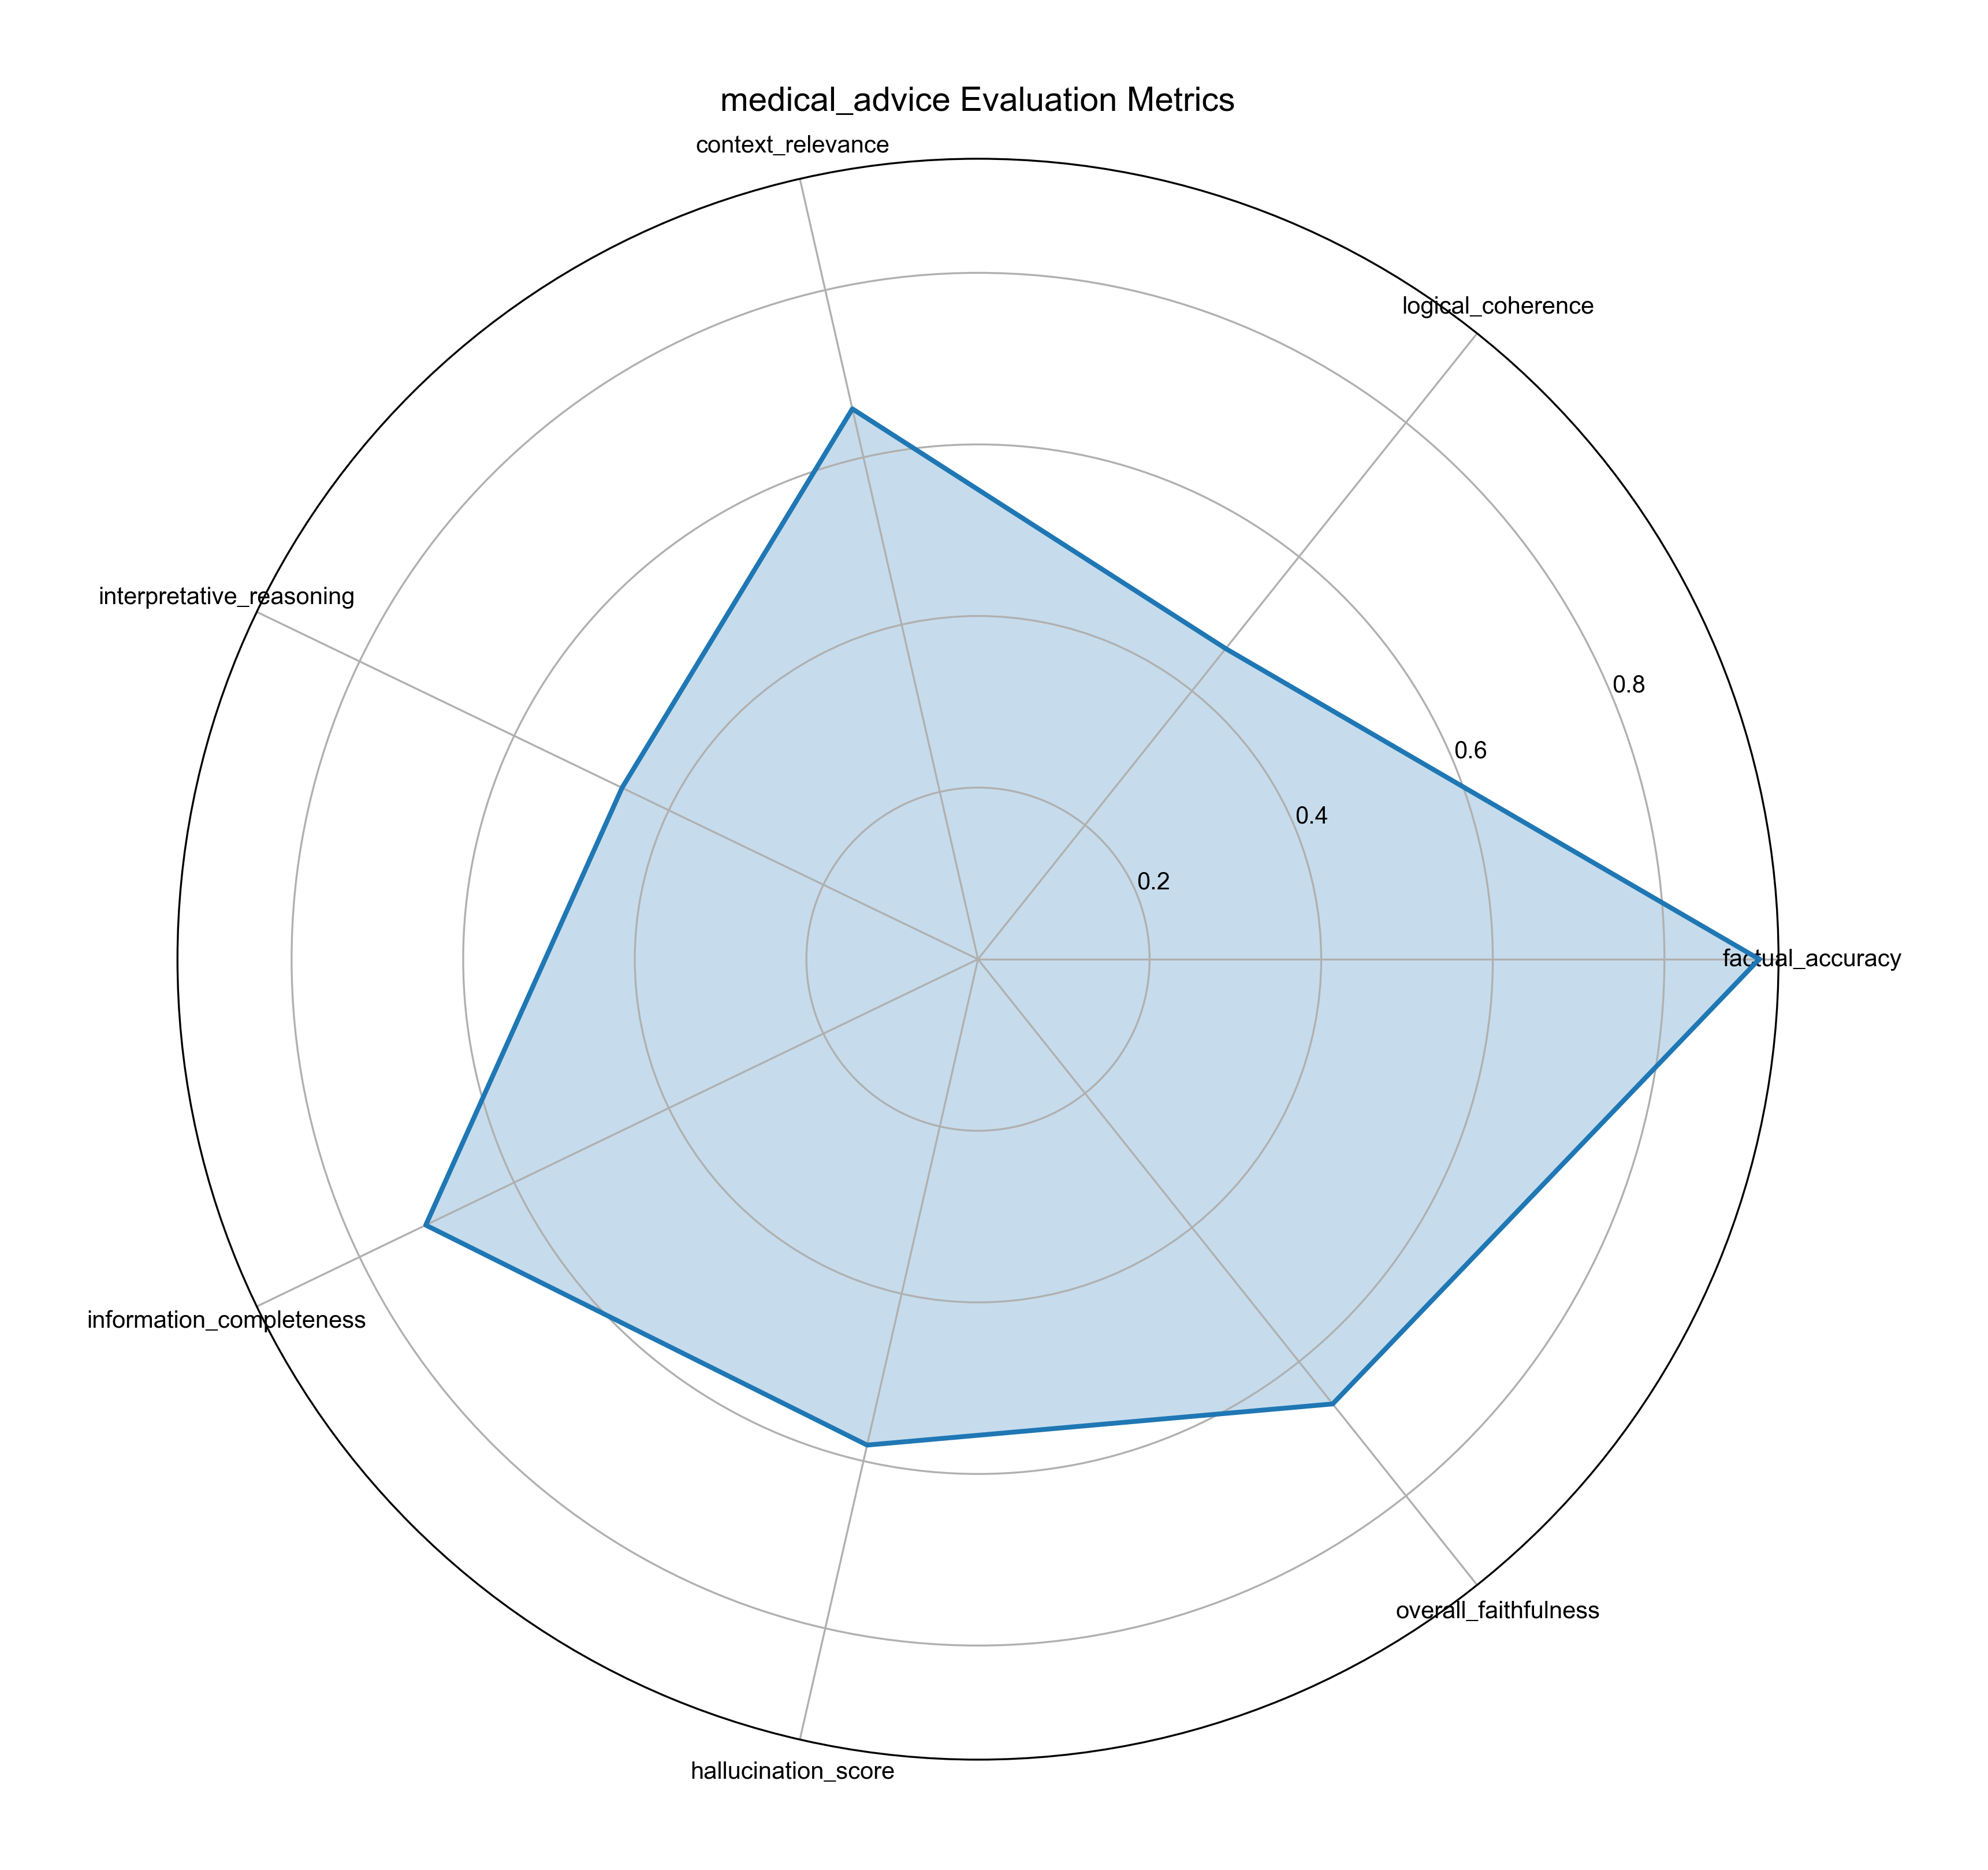
\includegraphics[width=0.6\textwidth]{figures/types/medical_advice_radar_gpt-4.png}
\caption{Medical Advice Performance Radar}
\label{fig:medical_radar}
\end{figure}

\textbf{Analysis}:
\begin{itemize}
    \item Notably high factual accuracy across all models, particularly in GPT-3.5-Turbo (0.9213)
    \item Strong information completeness scores reflect comprehensive medical responses
    \item Higher hallucination scores warrant attention in medical context
\end{itemize}

\subsubsection{Historical Analysis}
The historical analysis evaluation focused on the models' ability to accurately interpret and present historical information.

\begin{table}[!htbp]
\centering
\setlength{\tabcolsep}{4pt}  % Reduce table column spacing
\begin{tabular}{|l|c|c|c|c|c|c|c|}
\hline
\textbf{Model} & \textbf{FA} & \textbf{LC} & \textbf{CR} & \textbf{IR} 
& \textbf{IC} & \textbf{HS} & \textbf{OF} \\
\hline
GPT-3.5-Turbo & 0.82 & 0.17 & 0.70 & 0.59 & 0.79 & 0.11 & 0.56 \\
GPT-4-Turbo & 0.82 & 0.20 & 0.76 & 0.60 & 0.72 & 0.11 & 0.57 \\
GPT-4 & 0.82 & 0.20 & 0.76 & 0.60 & 0.72 & 0.11 & 0.57 \\
\hline
\end{tabular}
\caption{Historical Analysis Metrics}
\label{tab:results_historical_metrics}
\begin{flushleft}
\small
FA: Factual Accuracy, LC: Logical Coherence, CR: Context Relevance,\\
IR: Interpretative Reasoning, IC: Information Completeness, HS: Hallucination Score, OF: Overall Faithfulness
\end{flushleft}
\end{table}

\begin{figure}[!htbp]
\centering
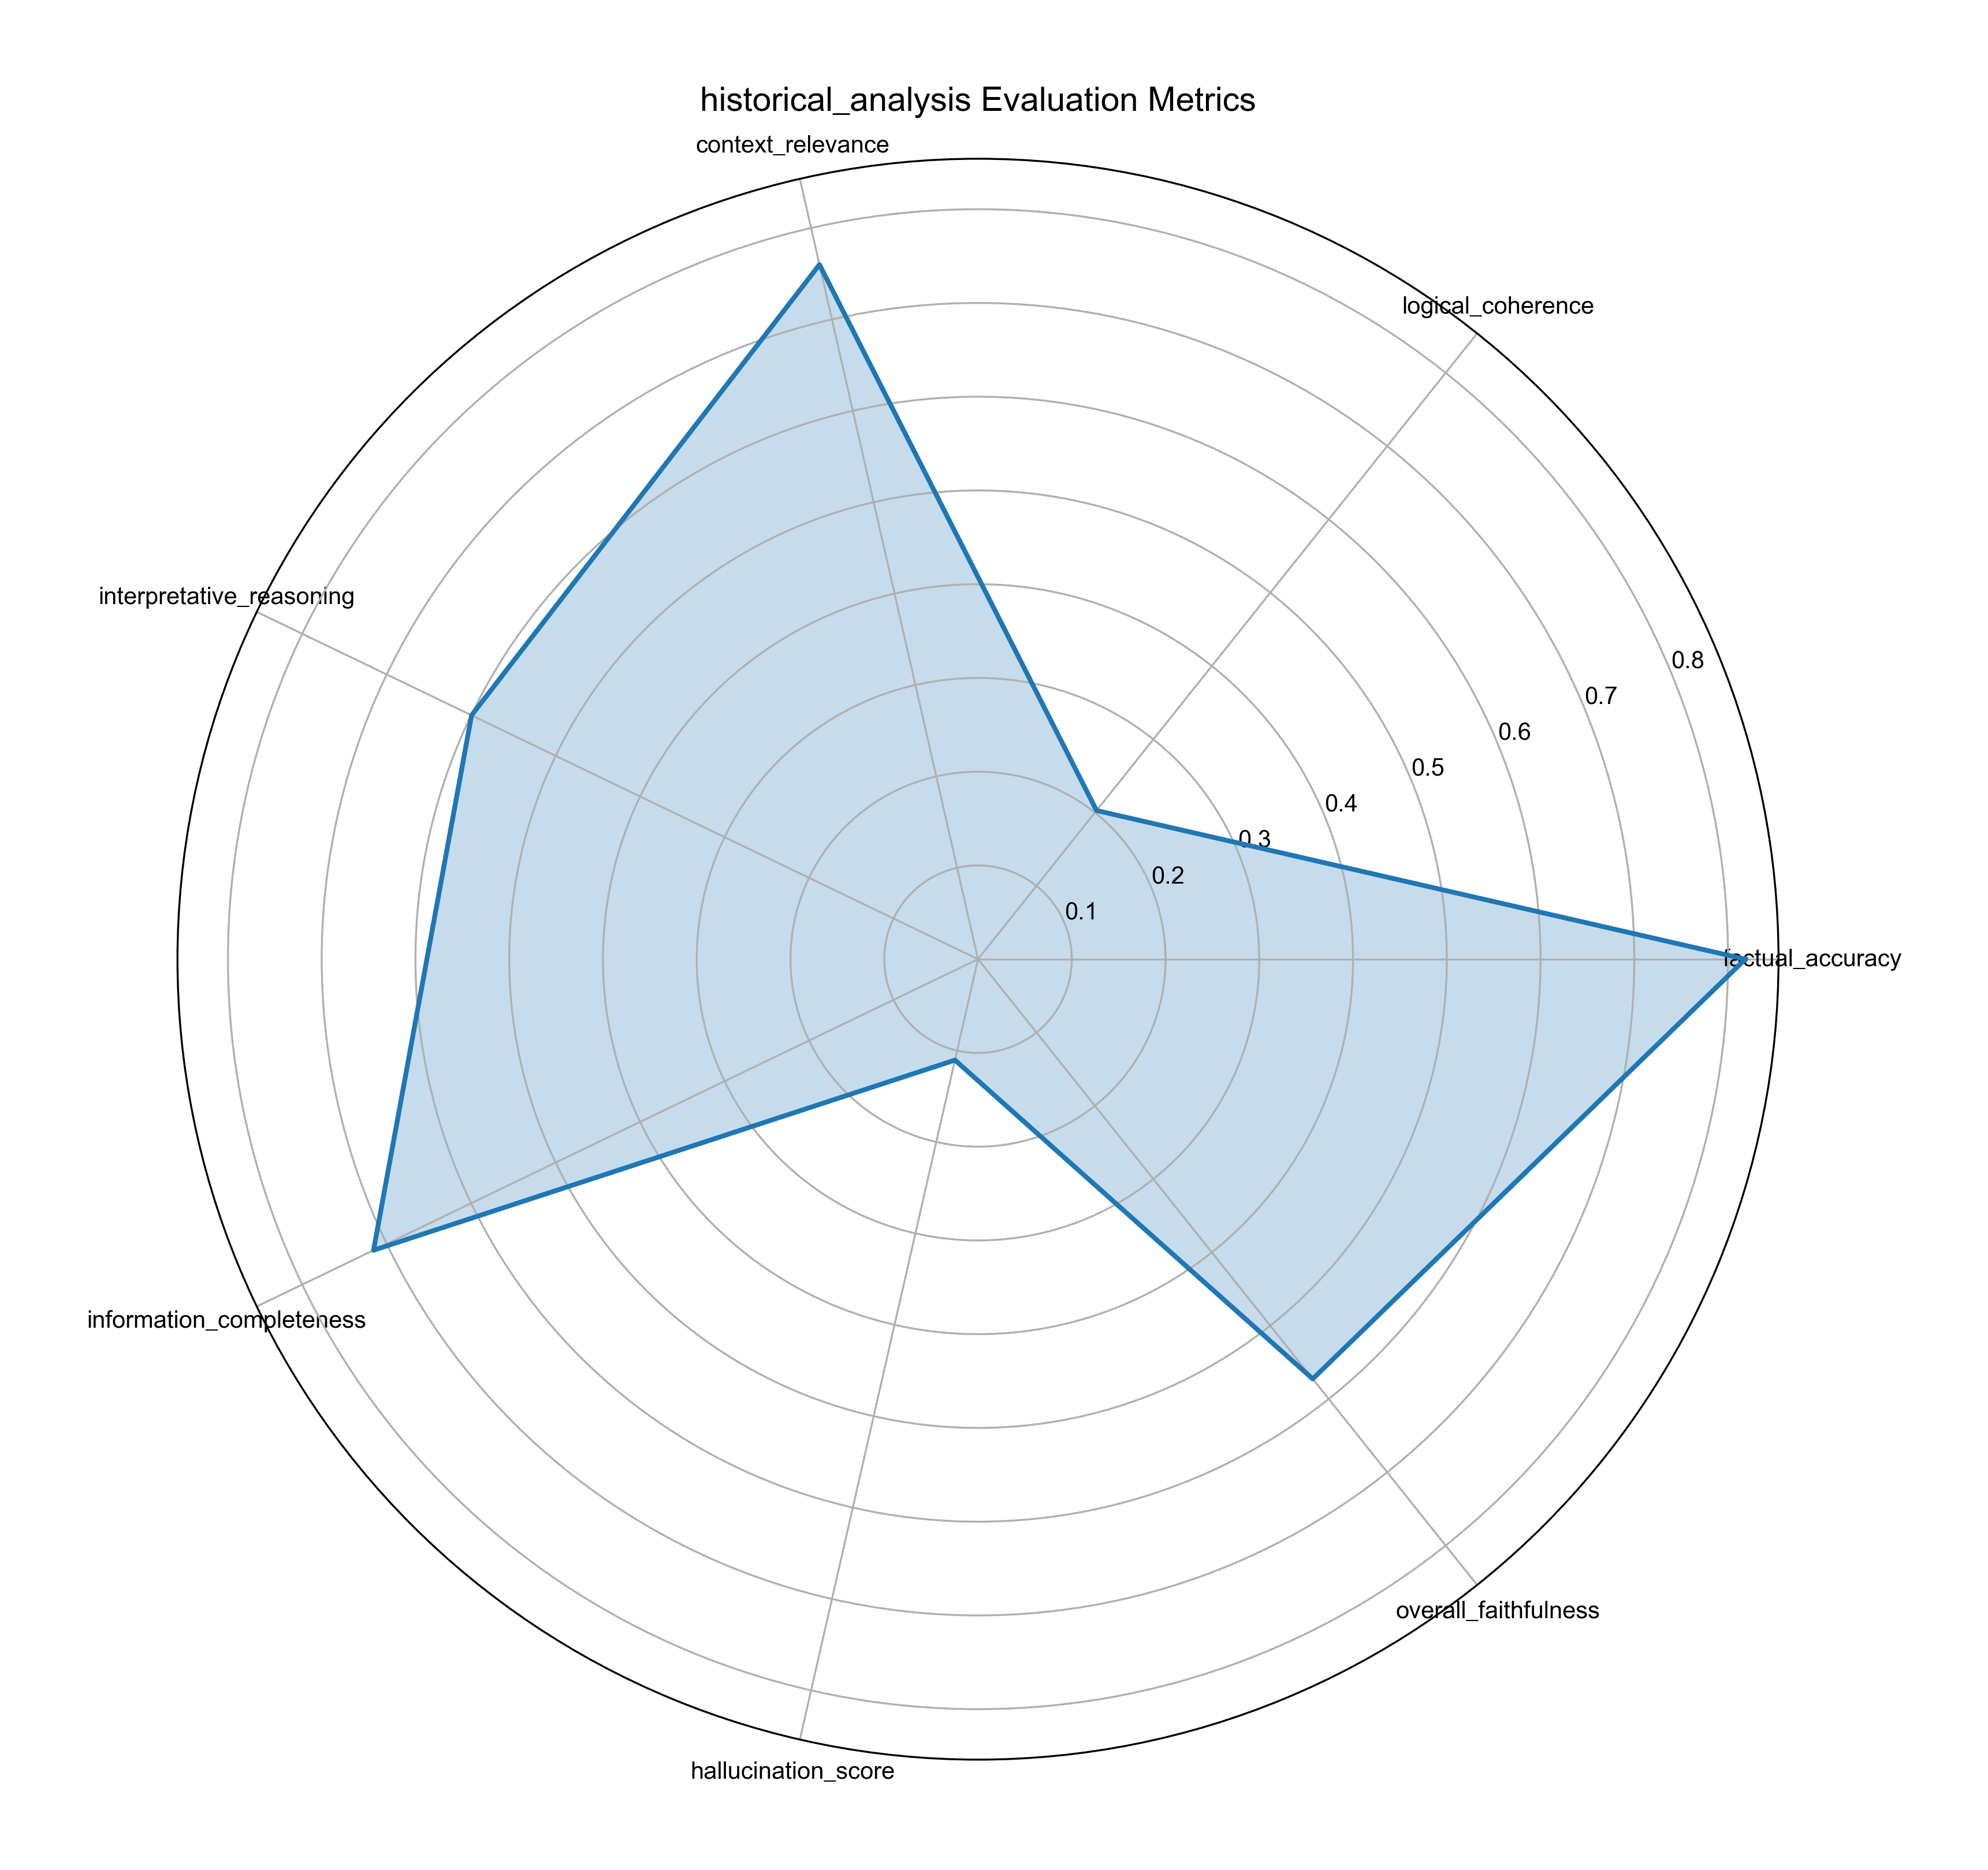
\includegraphics[width=0.6\textwidth]{figures/types/historical_analysis_radar_gpt-4.png}
\caption{Historical Analysis Performance Radar}
\label{fig:historical_radar}
\end{figure}

\textbf{Analysis}:
\begin{itemize}
    \item All models demonstrate consistent factual accuracy (0.82) in historical content
    \item Strong context relevance scores (>0.70) indicate good historical context understanding
    \item Lower logical coherence scores suggest challenges in organizing historical narratives
    \item Notably low hallucination scores (0.11) indicate reliable historical information presentation
\end{itemize}

\subsubsection{Current Events}
The current events evaluation assessed the models' ability to handle contemporary information and recent developments.

\begin{table}[!htbp]
\centering
\setlength{\tabcolsep}{4pt}  % Reduce table column spacing
\begin{tabular}{|l|c|c|c|c|c|c|c|}
\hline
\textbf{Model} & \textbf{FA} & \textbf{LC} & \textbf{CR} & \textbf{IR} 
& \textbf{IC} & \textbf{HS} & \textbf{OF} \\
\hline
GPT-3.5-Turbo & 0.80 & 0.52 & 0.43 & 0.54 & 0.66 & 0.51 & 0.61 \\
GPT-4-Turbo & 0.76 & 0.39 & 0.44 & 0.66 & 0.67 & 0.33 & 0.59 \\
GPT-4 & 0.78 & 0.45 & 0.44 & 0.66 & 0.67 & 0.33 & 0.59 \\
\hline
\end{tabular}
\caption{Current Events Metrics}
\label{tab:results_current_events_metrics}
\begin{flushleft}
\small
FA: Factual Accuracy, LC: Logical Coherence, CR: Context Relevance,\\
IR: Interpretative Reasoning, IC: Information Completeness, HS: Hallucination Score, OF: Overall Faithfulness
\end{flushleft}
\end{table}

\begin{figure}[!htbp]
\centering
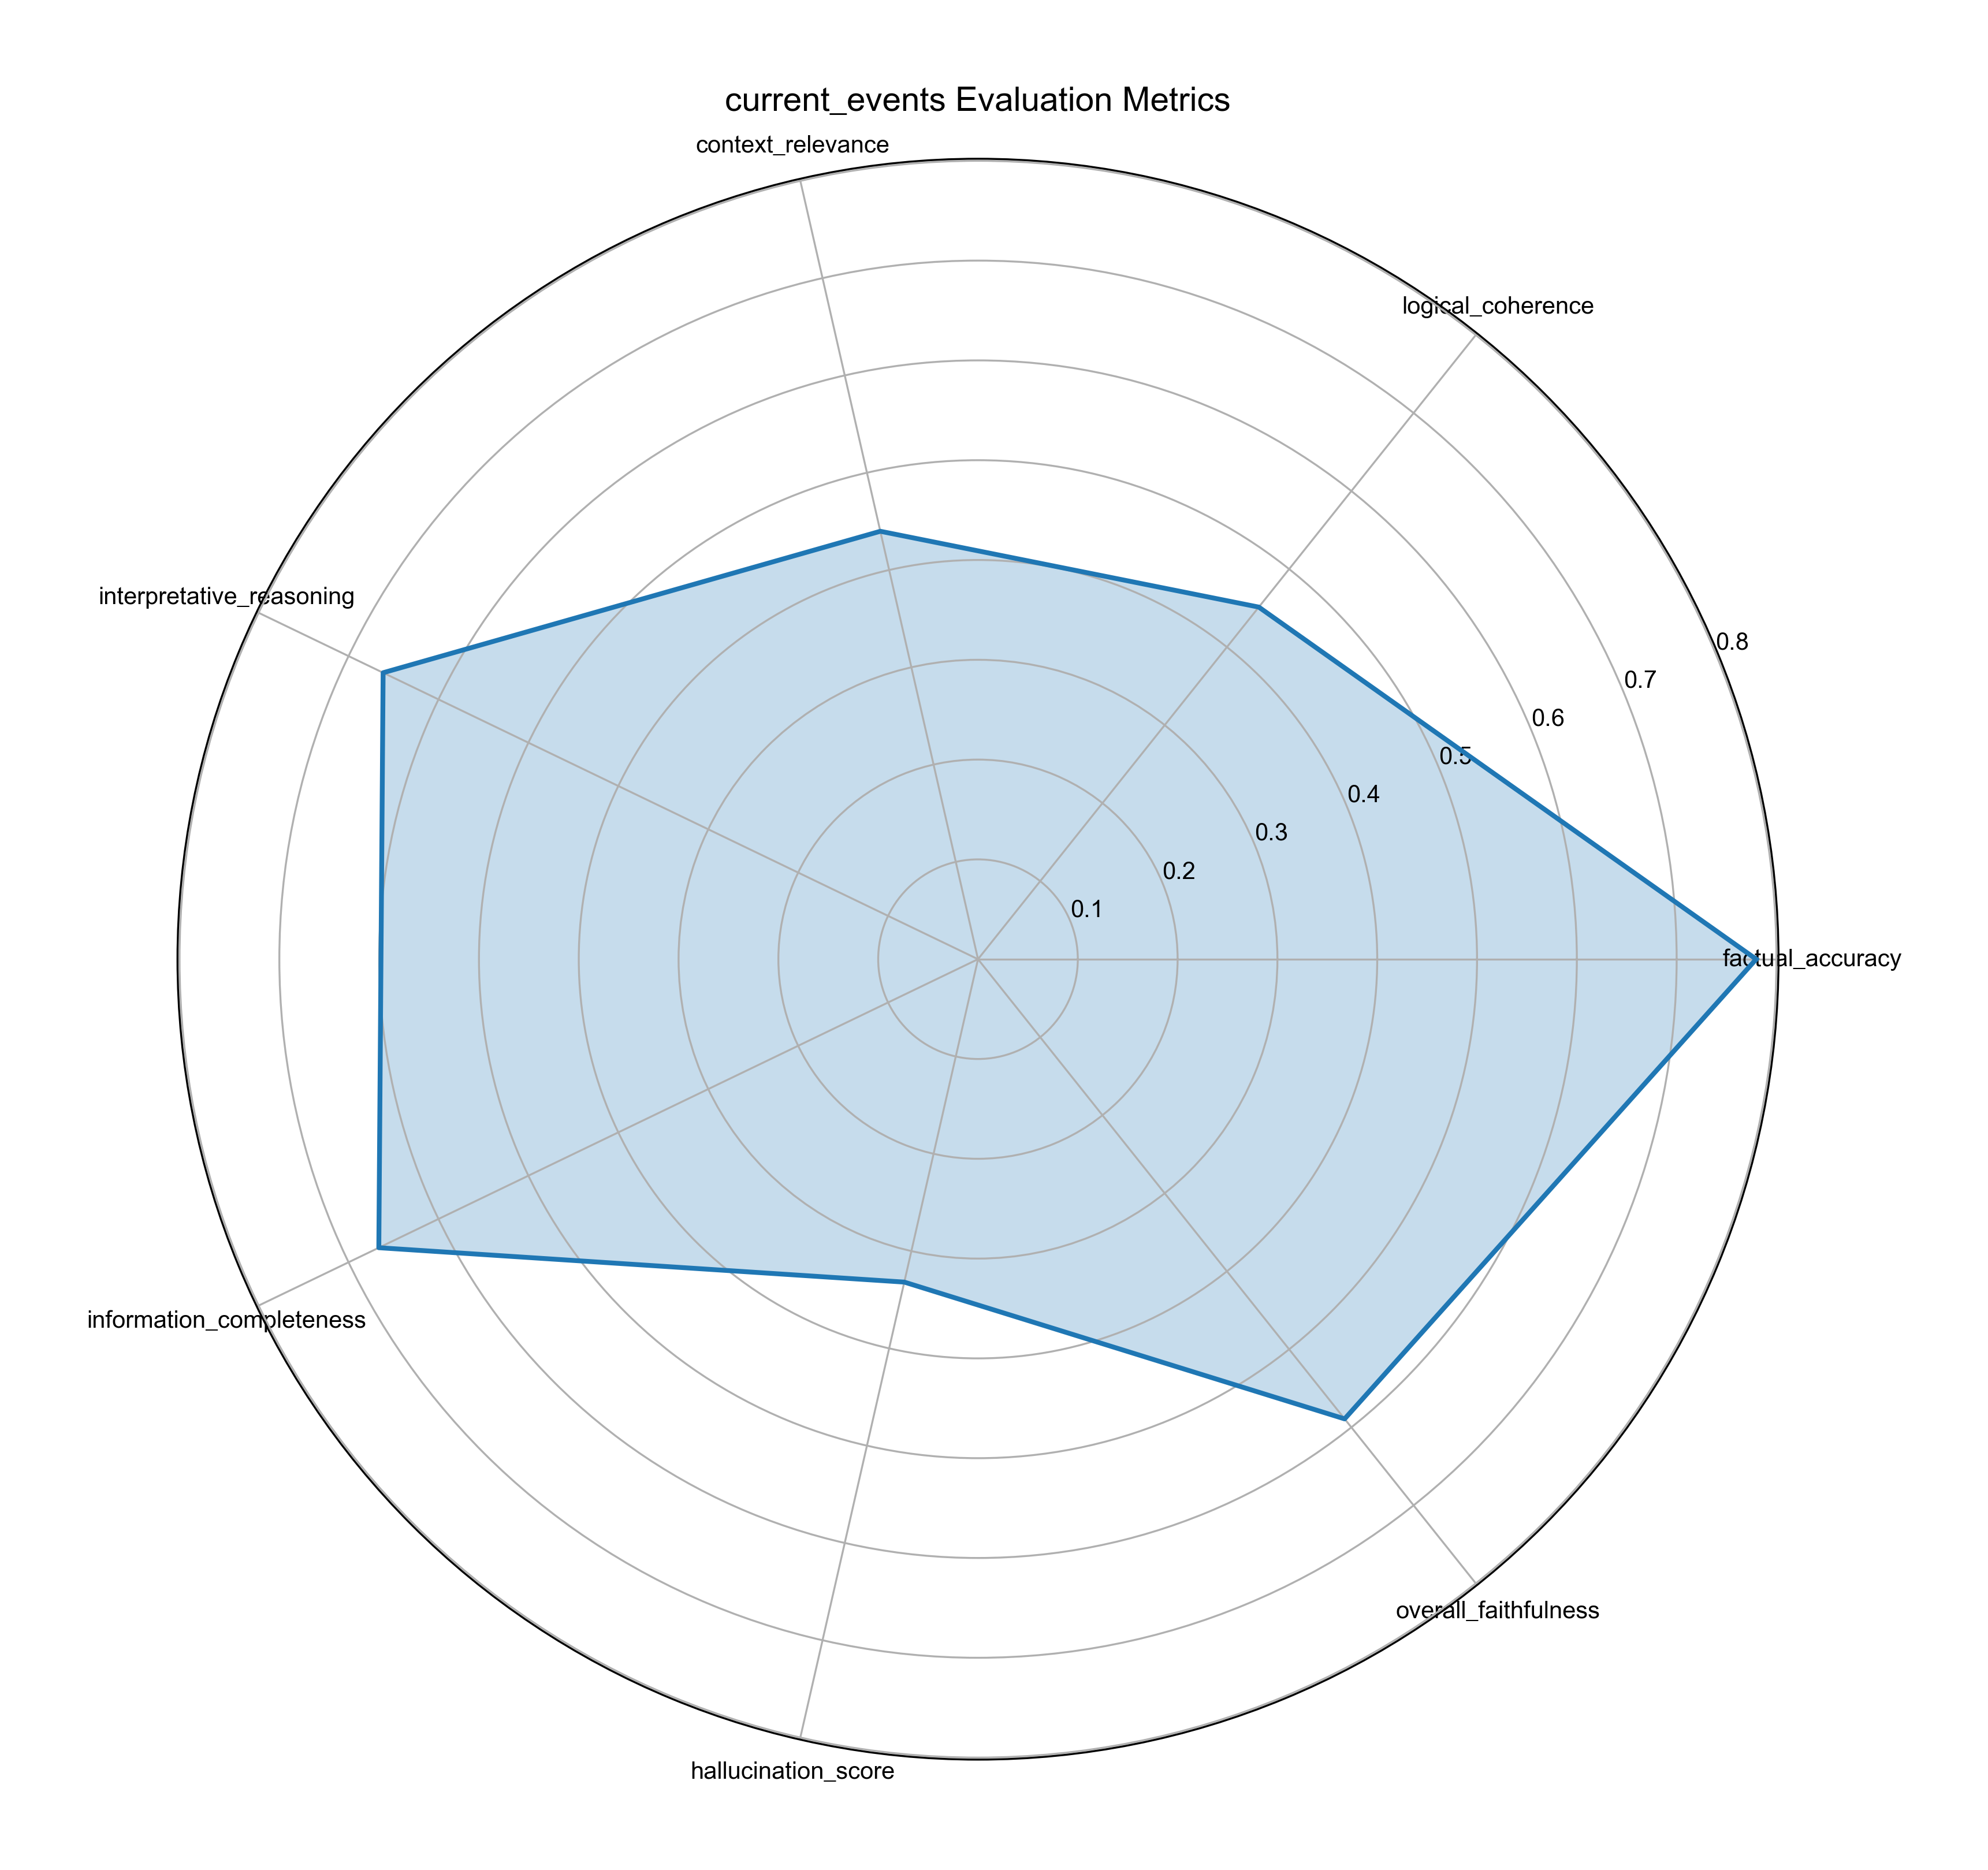
\includegraphics[width=0.6\textwidth]{figures/types/current_events_radar_gpt-4.png}
\caption{Current Events Performance Radar}
\label{fig:current_events_radar}
\end{figure}

\textbf{Analysis}:
\begin{itemize}
    \item GPT-3.5-Turbo shows highest factual accuracy (0.80) in current events
    \item Lower context relevance scores (<0.45) suggest challenges in connecting contemporary information
    \item Higher hallucination scores indicate increased uncertainty in recent event analysis
    \item Strong interpretative reasoning in GPT-4 variants (0.66) shows good analytical capabilities
\end{itemize}

\subsubsection{Sample Type Comparison}
A comprehensive comparison across different sample types reveals how models adapt to varying content domains.

\begin{figure}[!htbp]
\centering
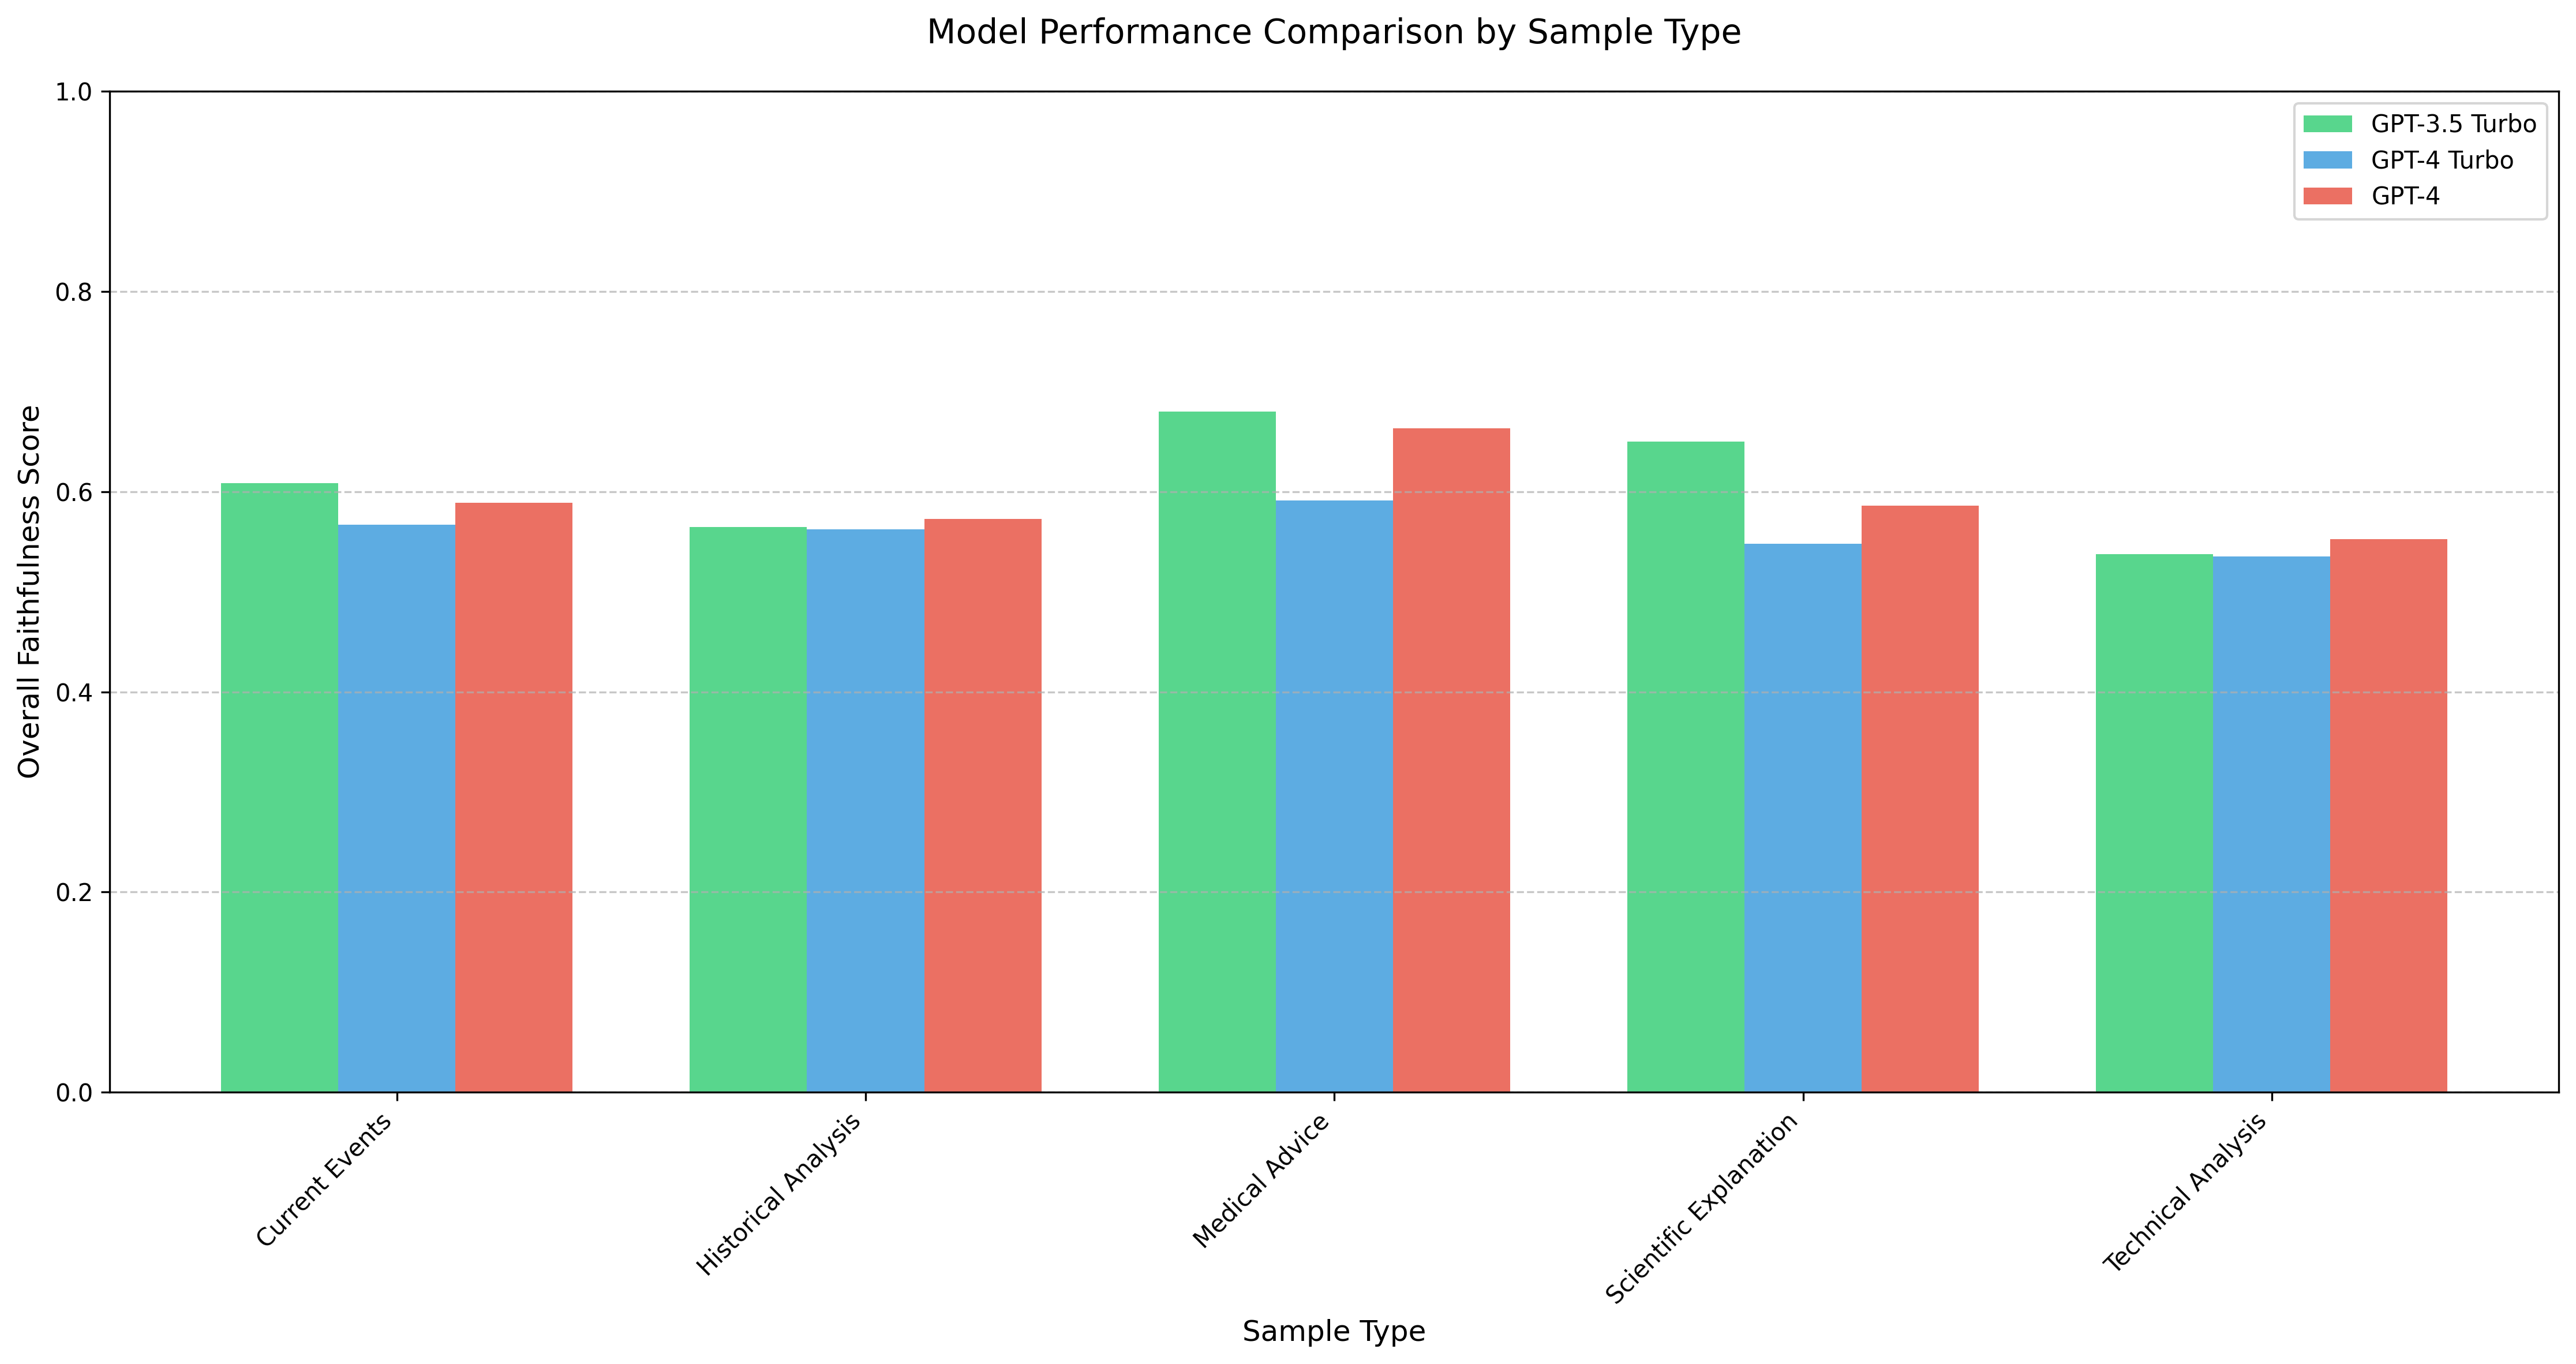
\includegraphics[width=0.8\textwidth]{figures/types/type_comparison.png}
\caption{Performance Comparison Across Sample Types}
\label{fig:type_comparison}
\end{figure}

\textbf{Cross-Type Analysis}:
\begin{itemize}
    \item Different content types present unique challenges for each model
    \item Performance patterns vary significantly across domains
    \item Some metrics show consistent trends regardless of content type
\end{itemize}

\subsection{Visualization Analysis}

\subsubsection{Metric Distribution Analysis}
The box plots provide insights into the statistical distribution and variability of each metric across models.

\begin{figure}[!htbp]
\centering
\begin{subfigure}[b]{0.32\textwidth}
    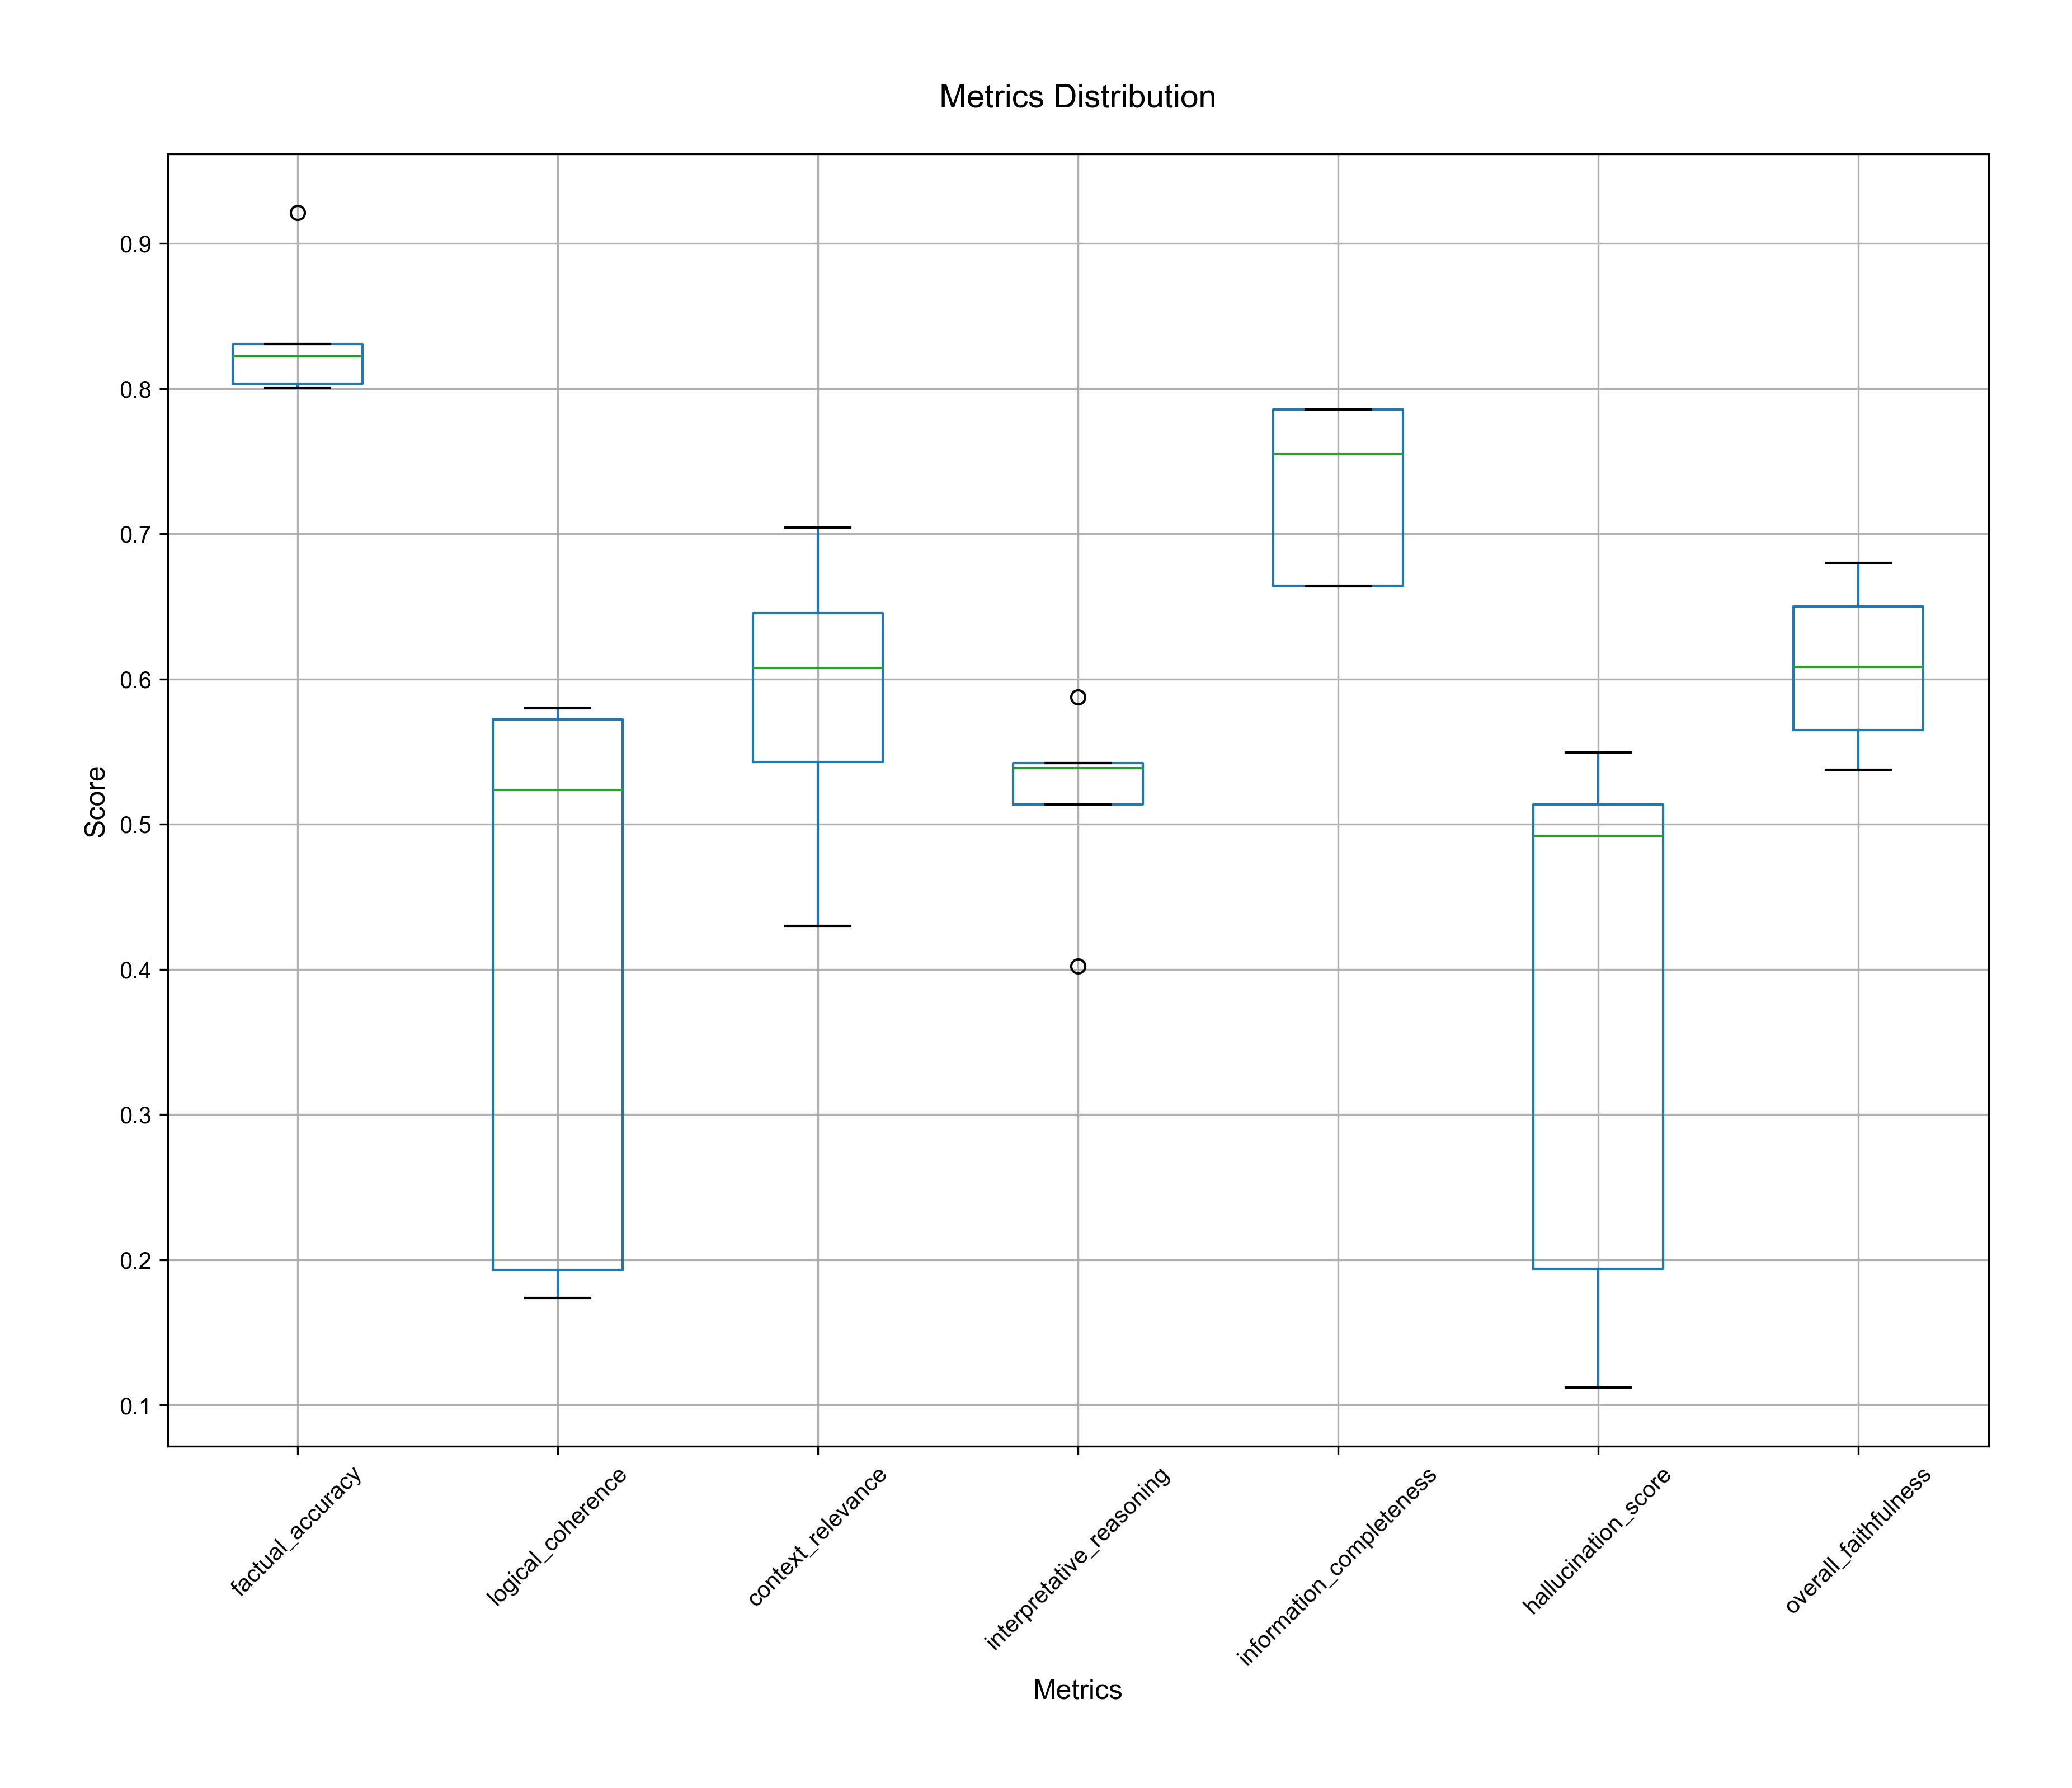
\includegraphics[width=\textwidth]{figures/visualization/metrics_boxplot_gpt-3.5-turbo.png}
    \caption{GPT-3.5-Turbo}
    \label{fig:metrics_boxplot_gpt35}
\end{subfigure}
\hfill
\begin{subfigure}[b]{0.32\textwidth}
    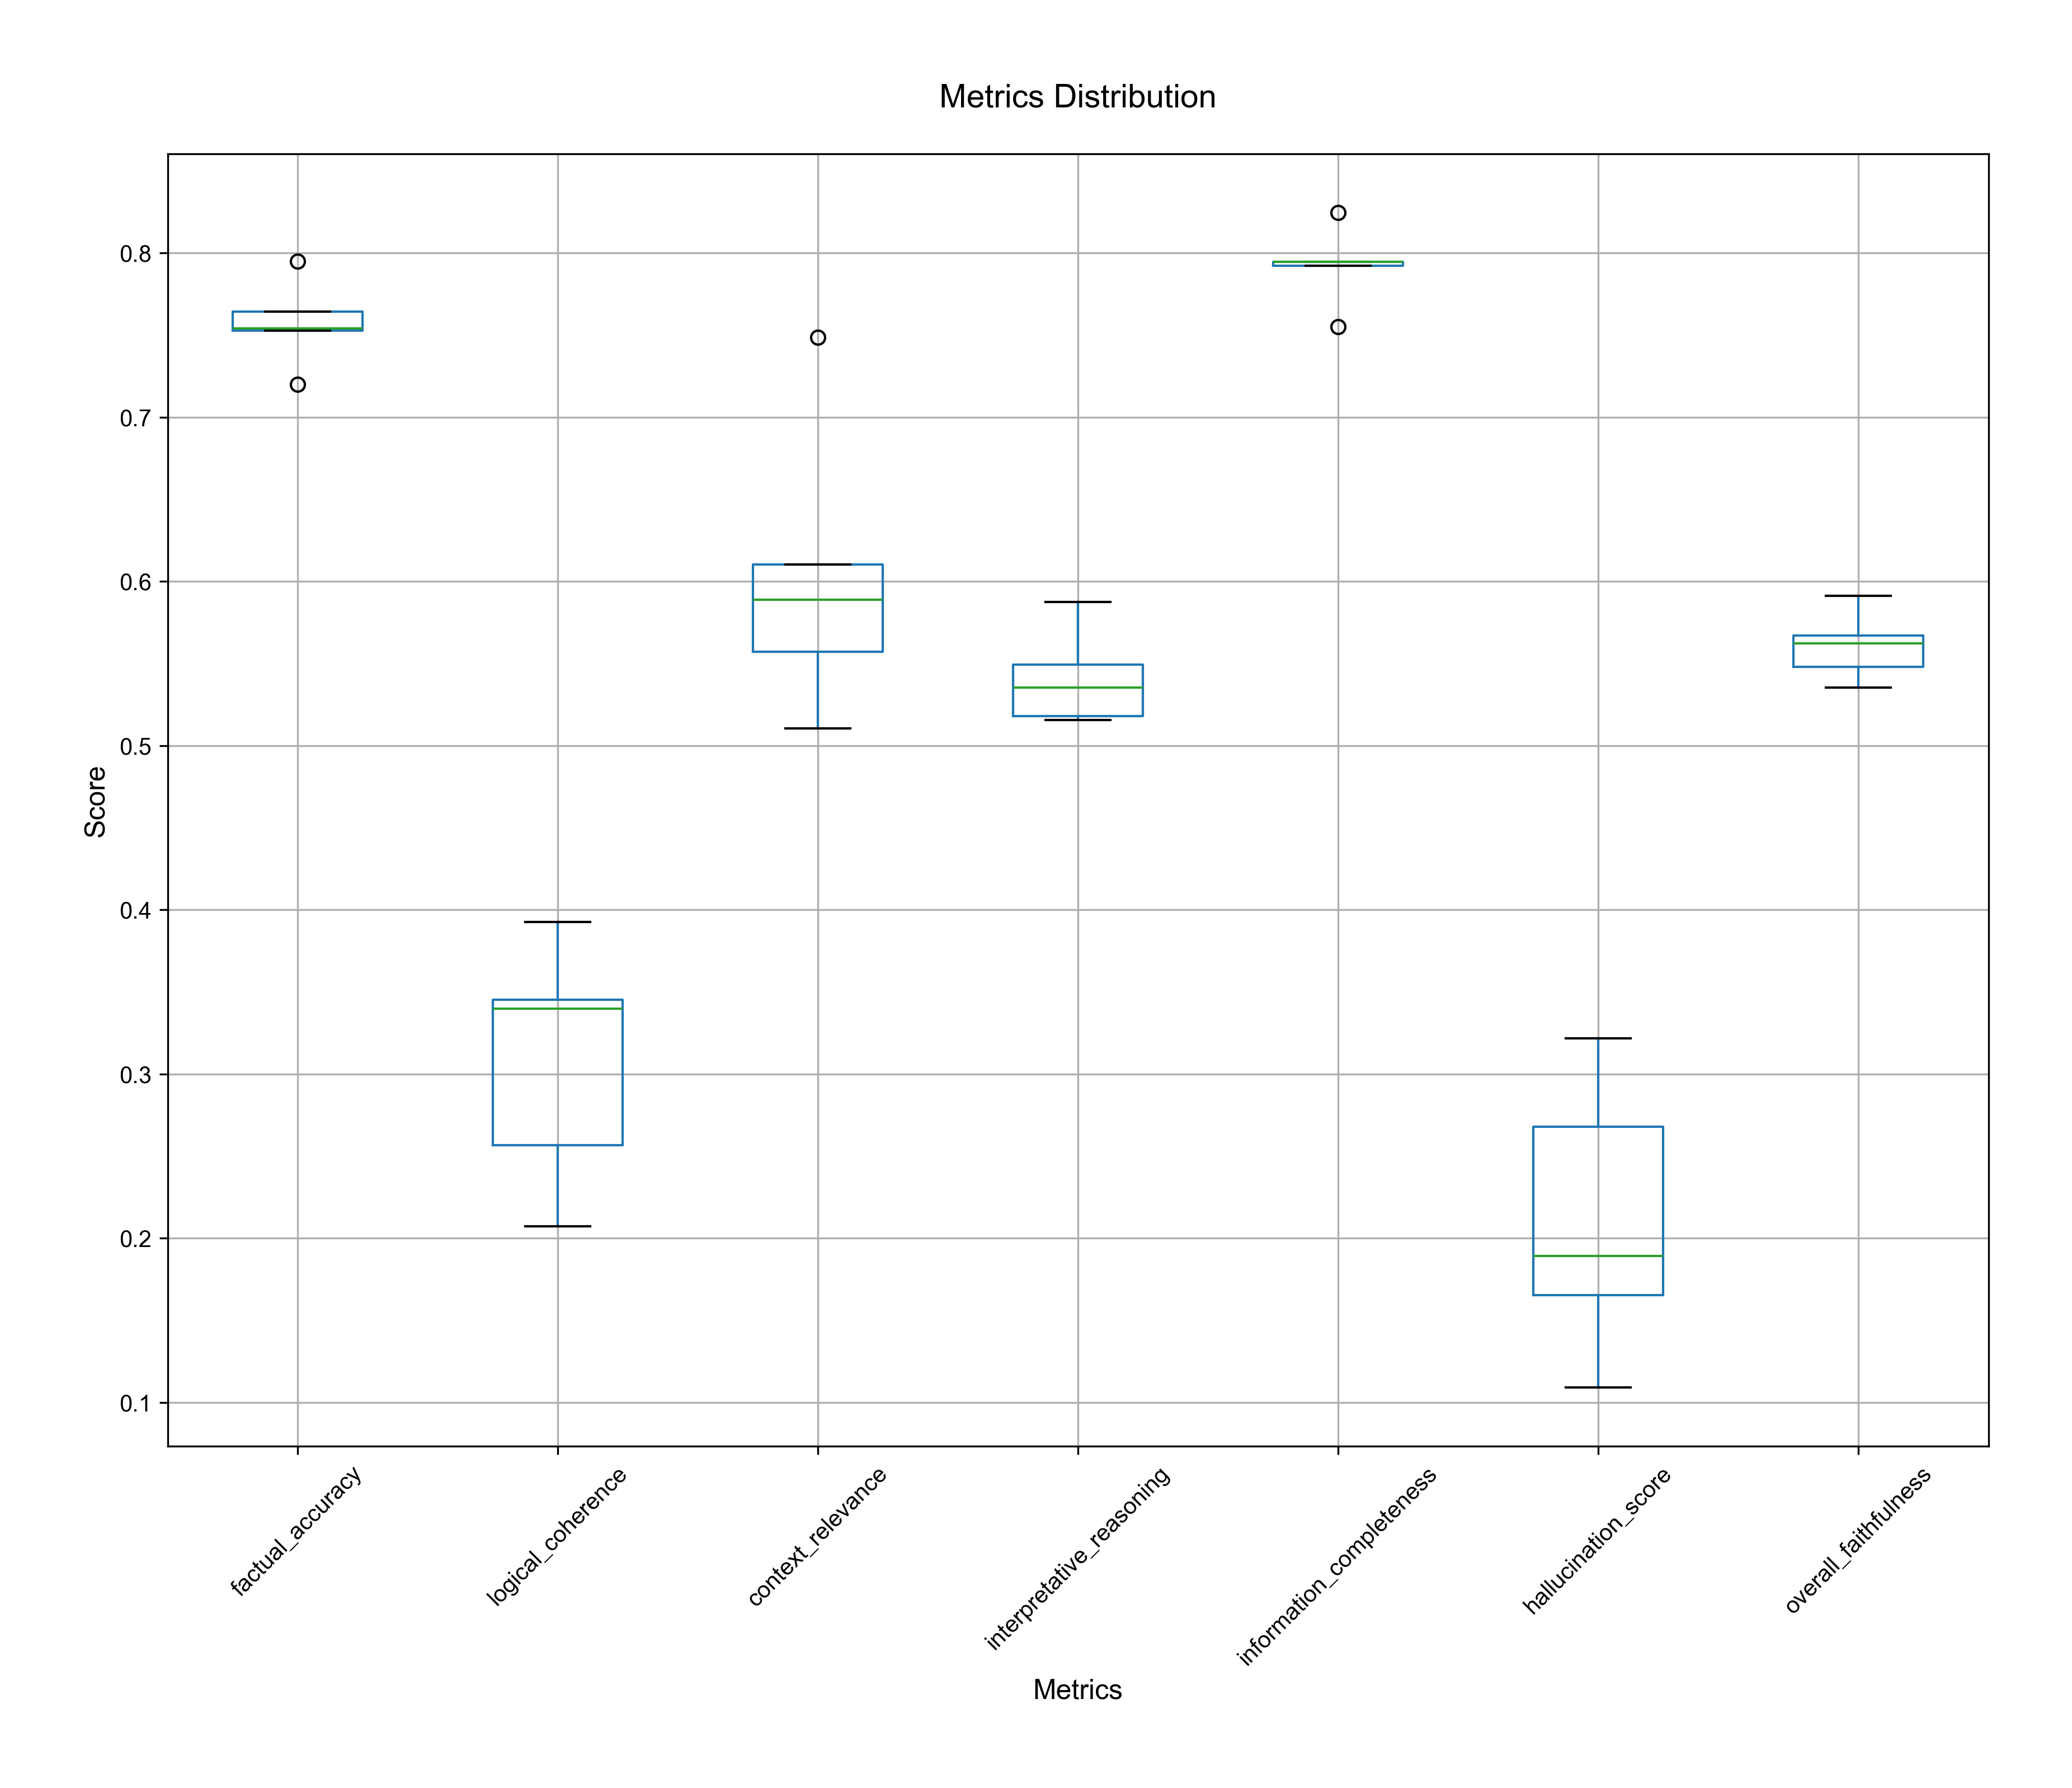
\includegraphics[width=\textwidth]{figures/visualization/metrics_boxplot_gpt-4-turbo.png}
    \caption{GPT-4-Turbo}
    \label{fig:metrics_boxplot_gpt4t}
\end{subfigure}
\hfill
\begin{subfigure}[b]{0.32\textwidth}
    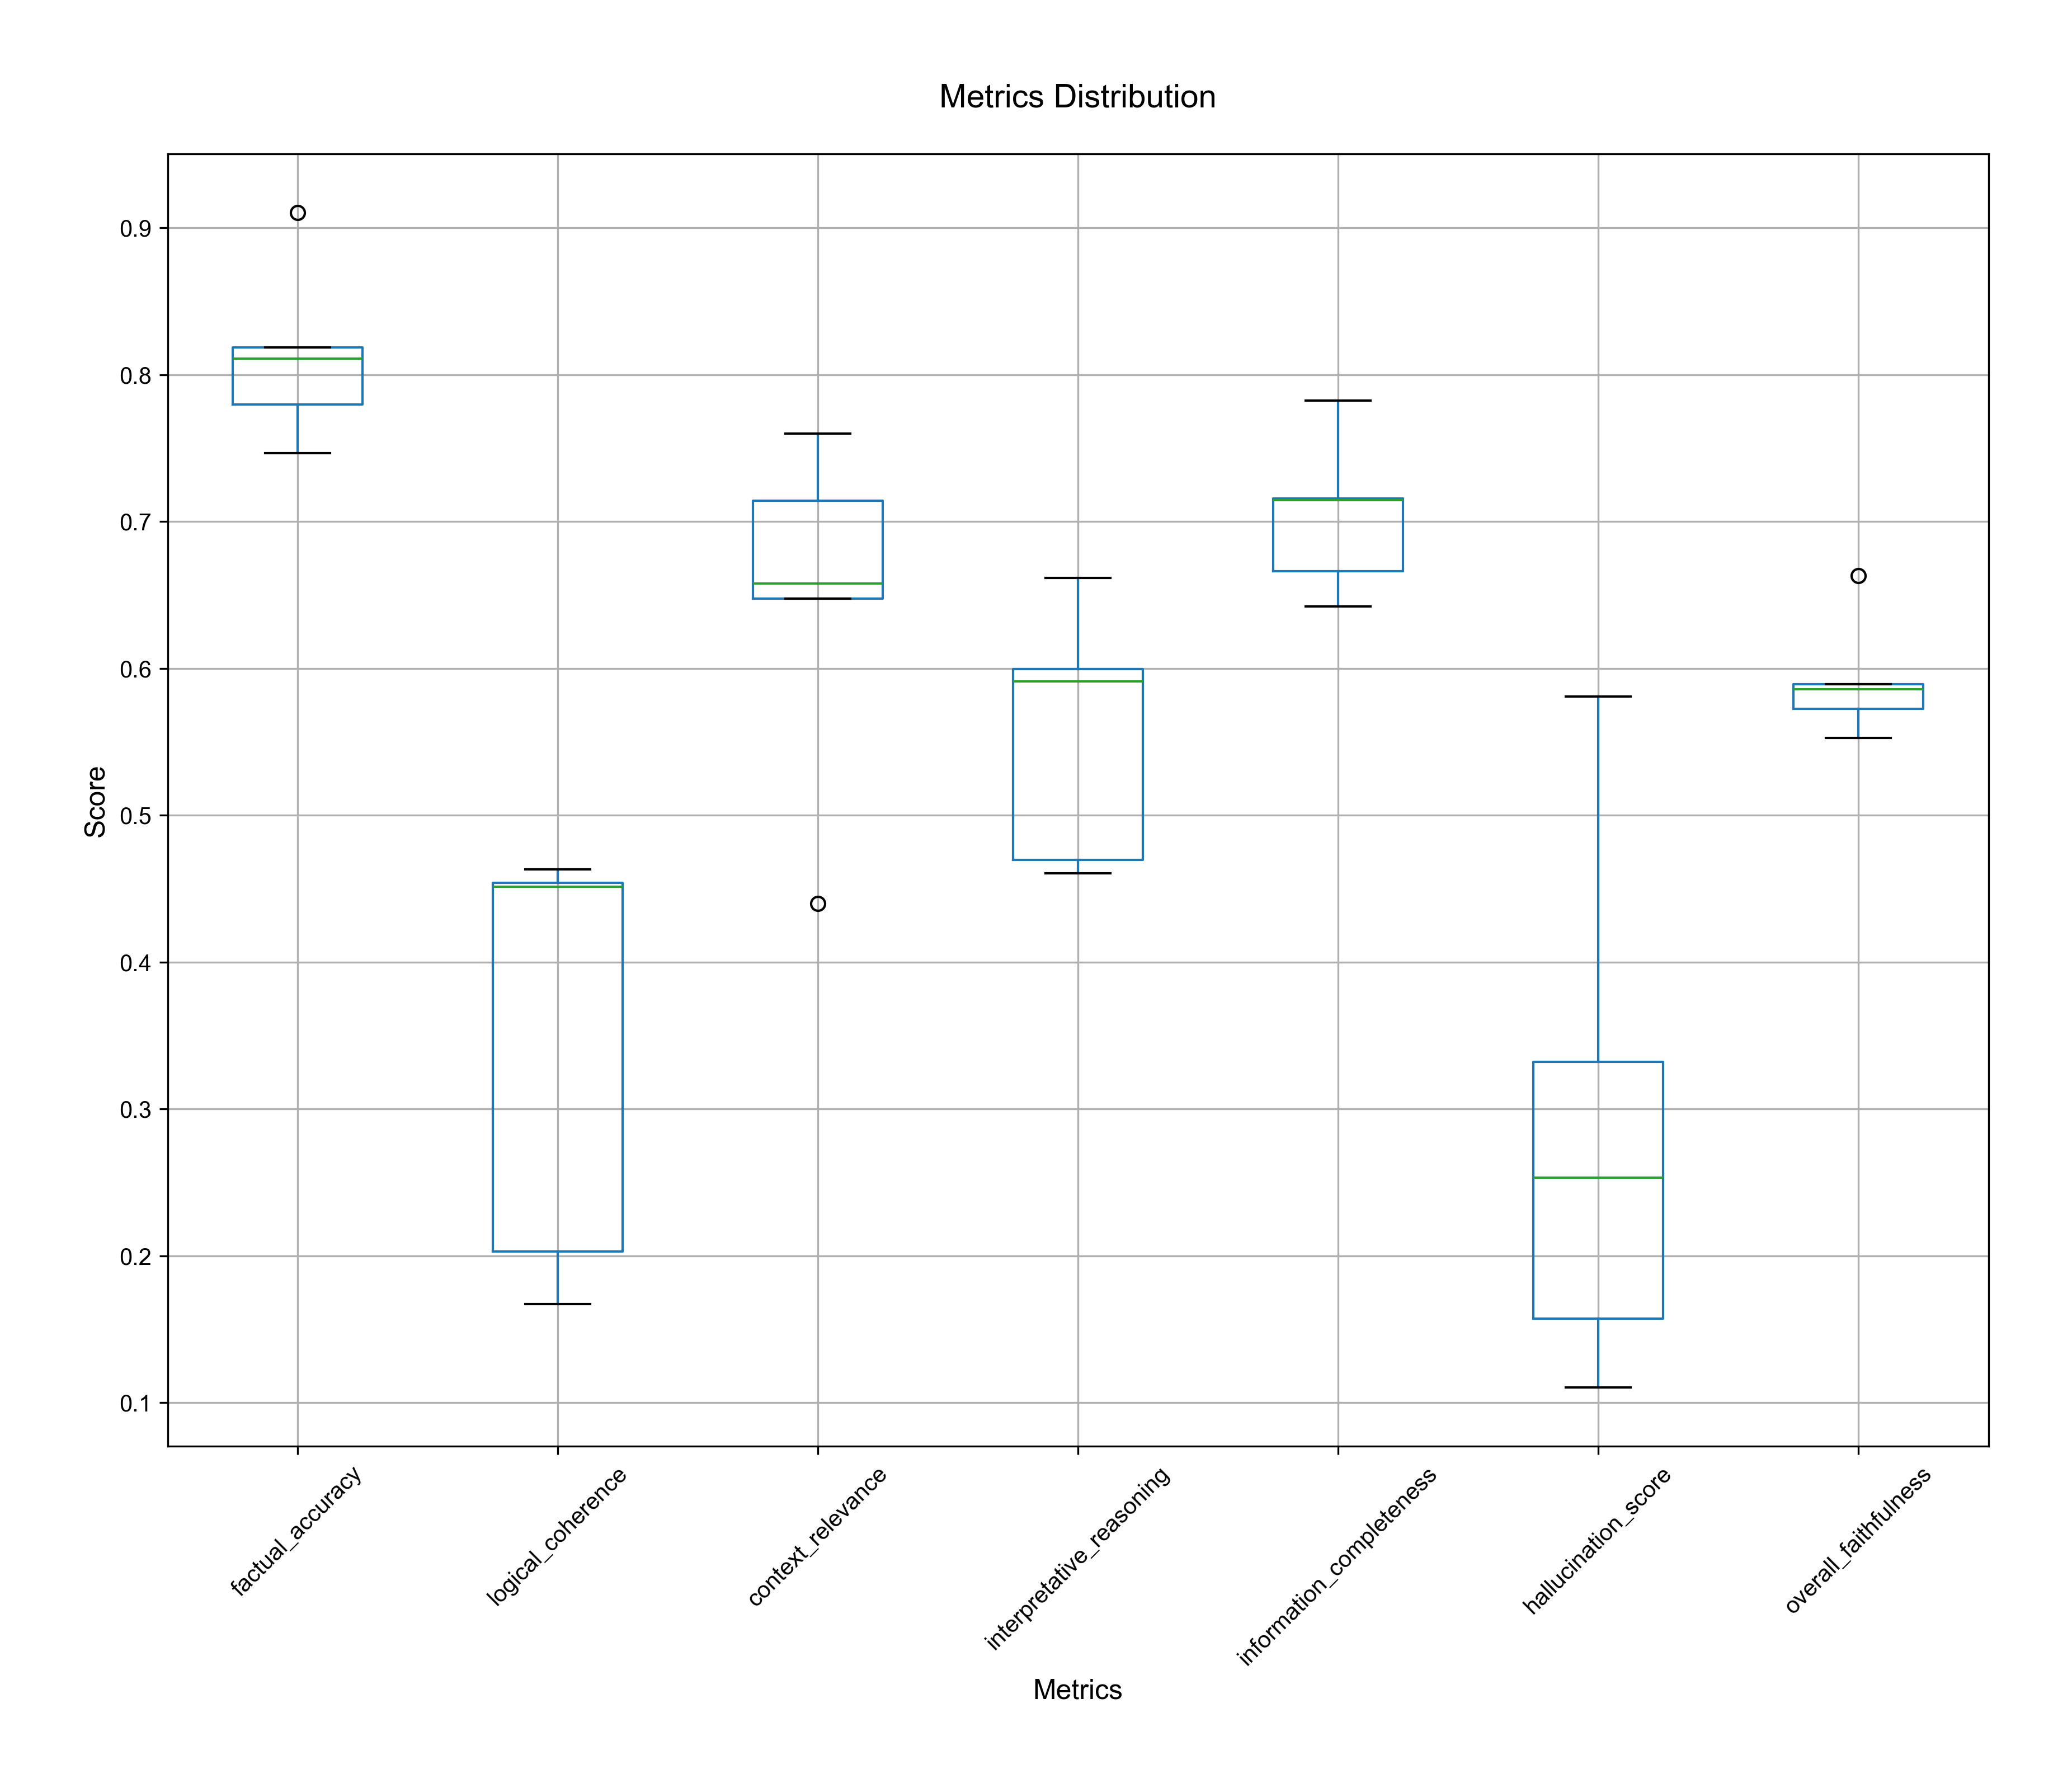
\includegraphics[width=\textwidth]{figures/visualization/metrics_boxplot_gpt-4.png}
    \caption{GPT-4}
    \label{fig:metrics_boxplot_gpt4}
\end{subfigure}
\caption{Metric Score Distributions by Model}
\label{fig:metrics_boxplots}
\end{figure}

\textbf{Distribution Insights}:
\begin{itemize}
    \item Factual accuracy shows the most consistent distribution across models
    \item Logical coherence exhibits the widest range of scores
    \item Hallucination scores show significant outliers, particularly in GPT-3.5-Turbo
\end{itemize}

\subsubsection{Correlation Analysis}
Heat maps visualize the relationships between different metrics, revealing important patterns and dependencies.

\begin{figure}[!htbp]
\centering
\begin{subfigure}[b]{0.32\textwidth}
    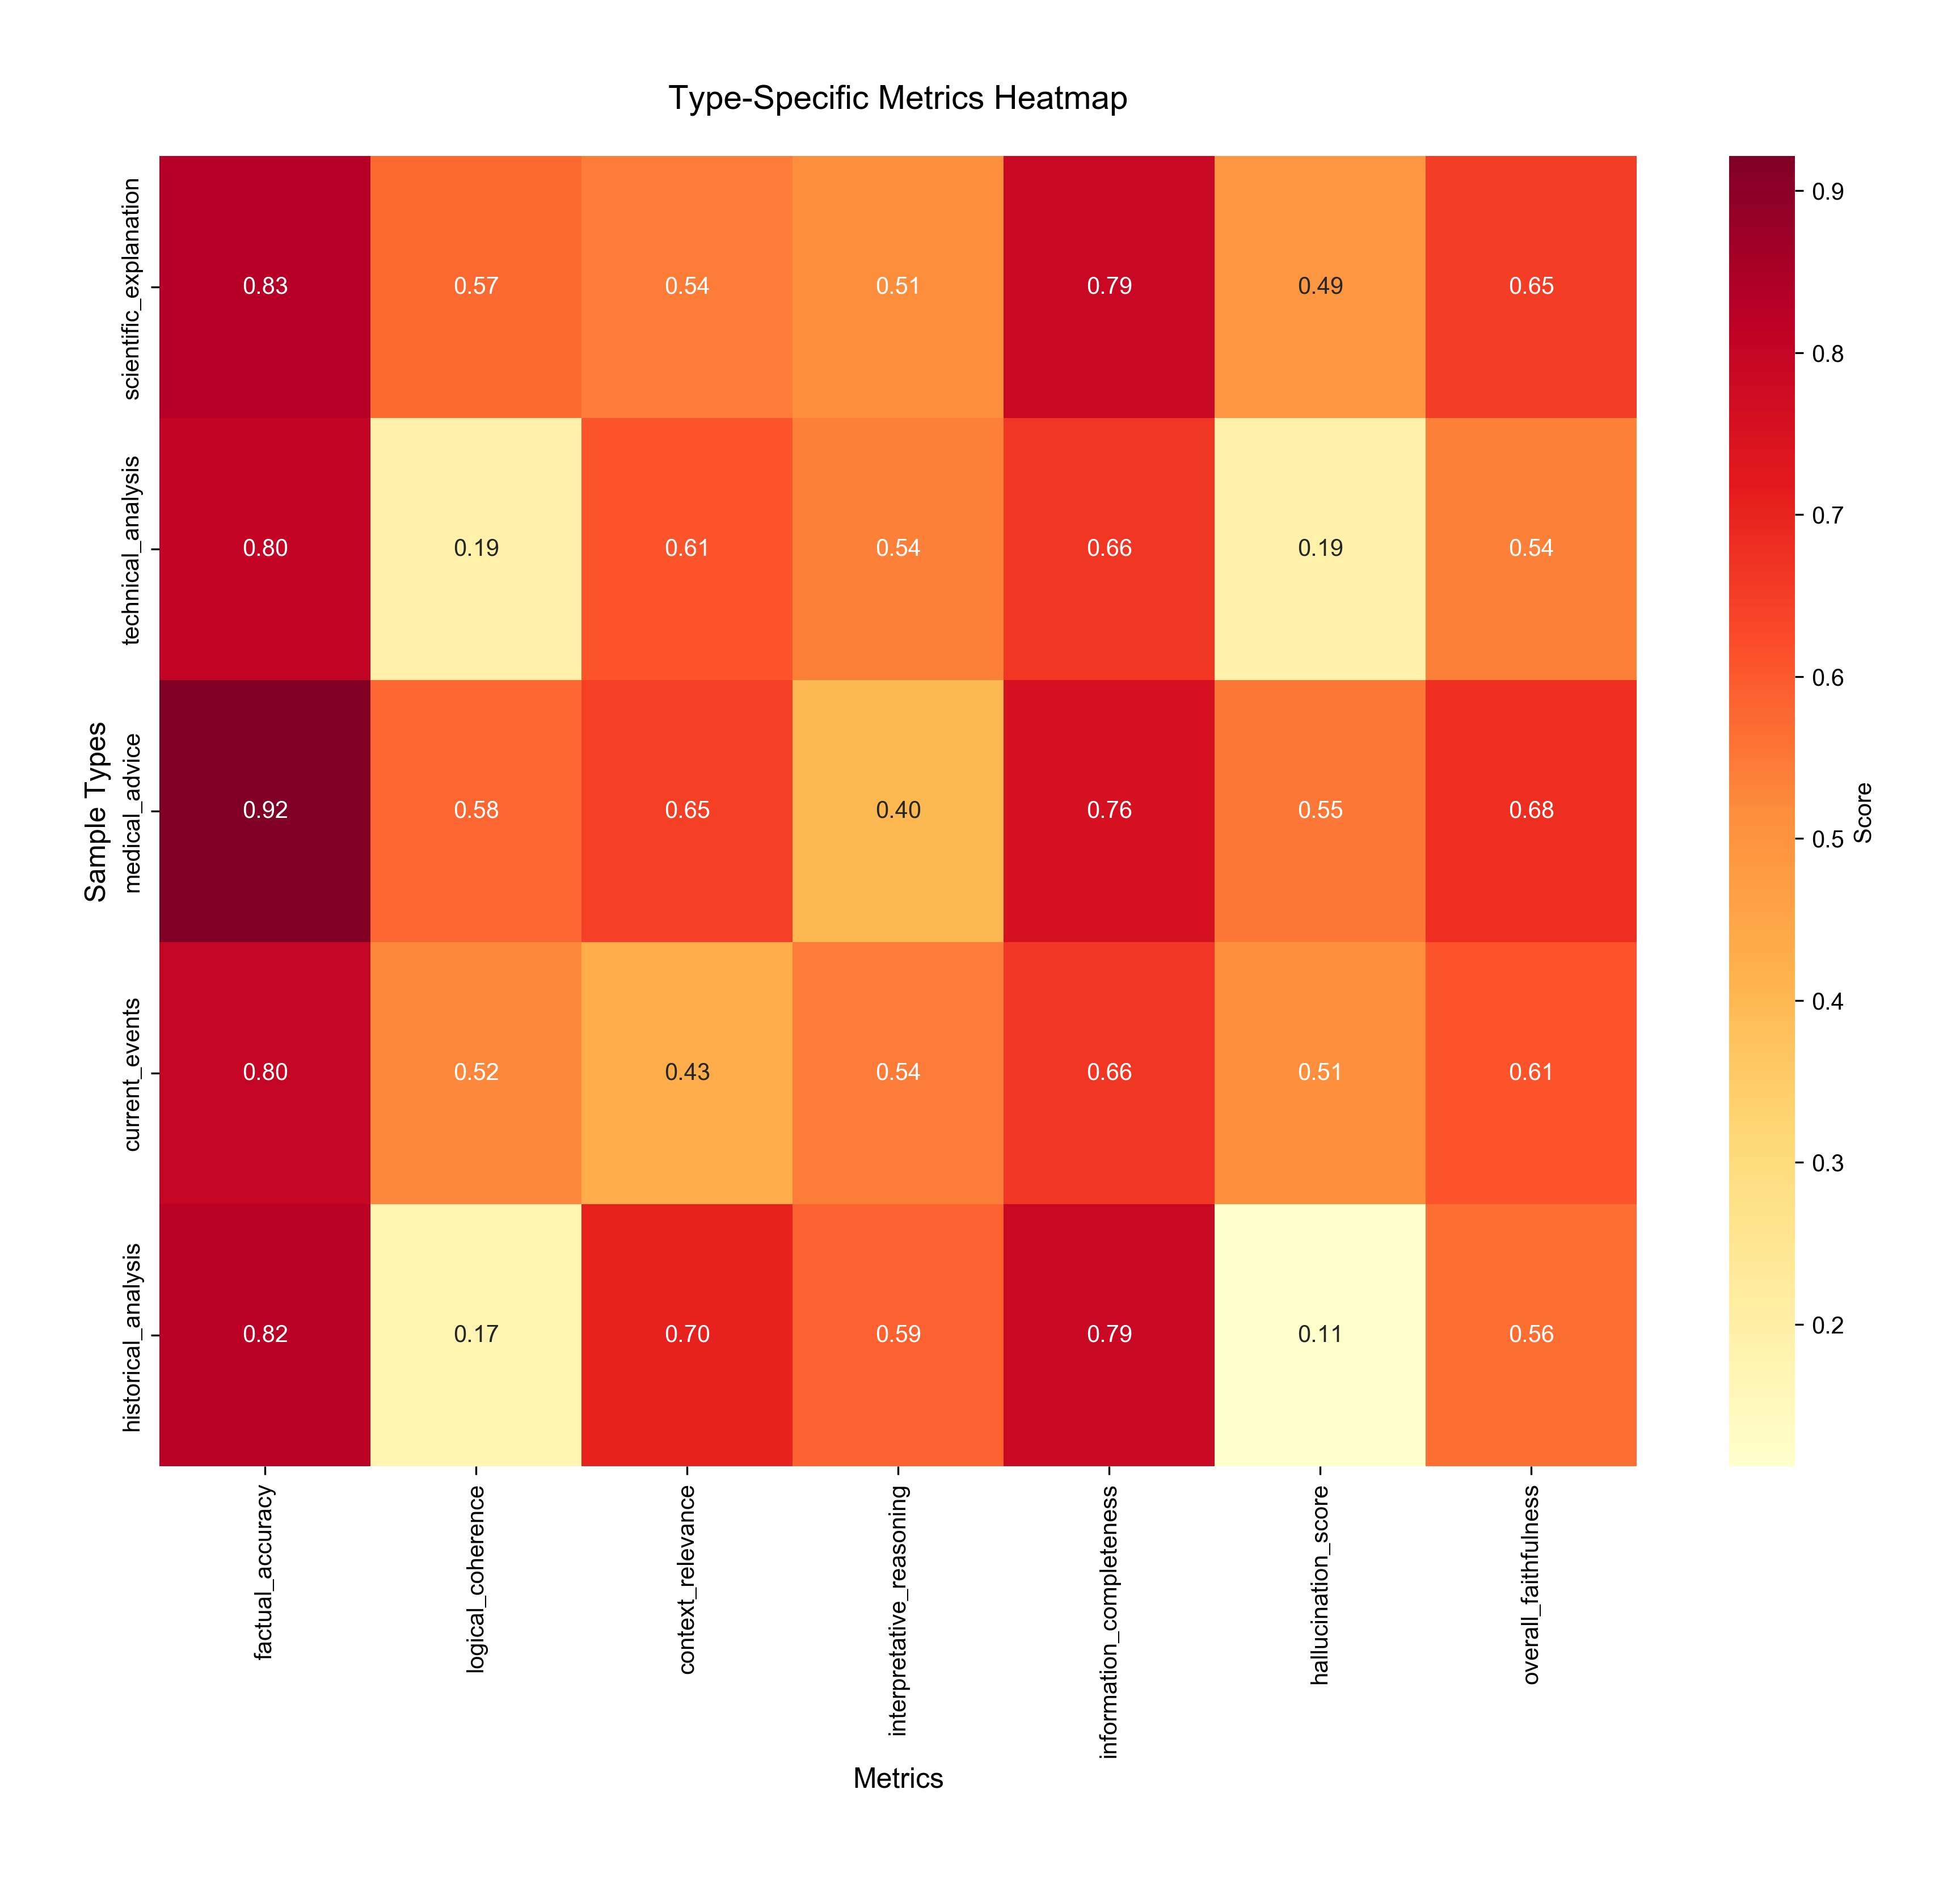
\includegraphics[width=\textwidth]{figures/visualization/metrics_heatmap_gpt-3.5-turbo.png}
    \caption{GPT-3.5-Turbo}
    \label{fig:metrics_heatmap_gpt35}
\end{subfigure}
\hfill
\begin{subfigure}[b]{0.32\textwidth}
    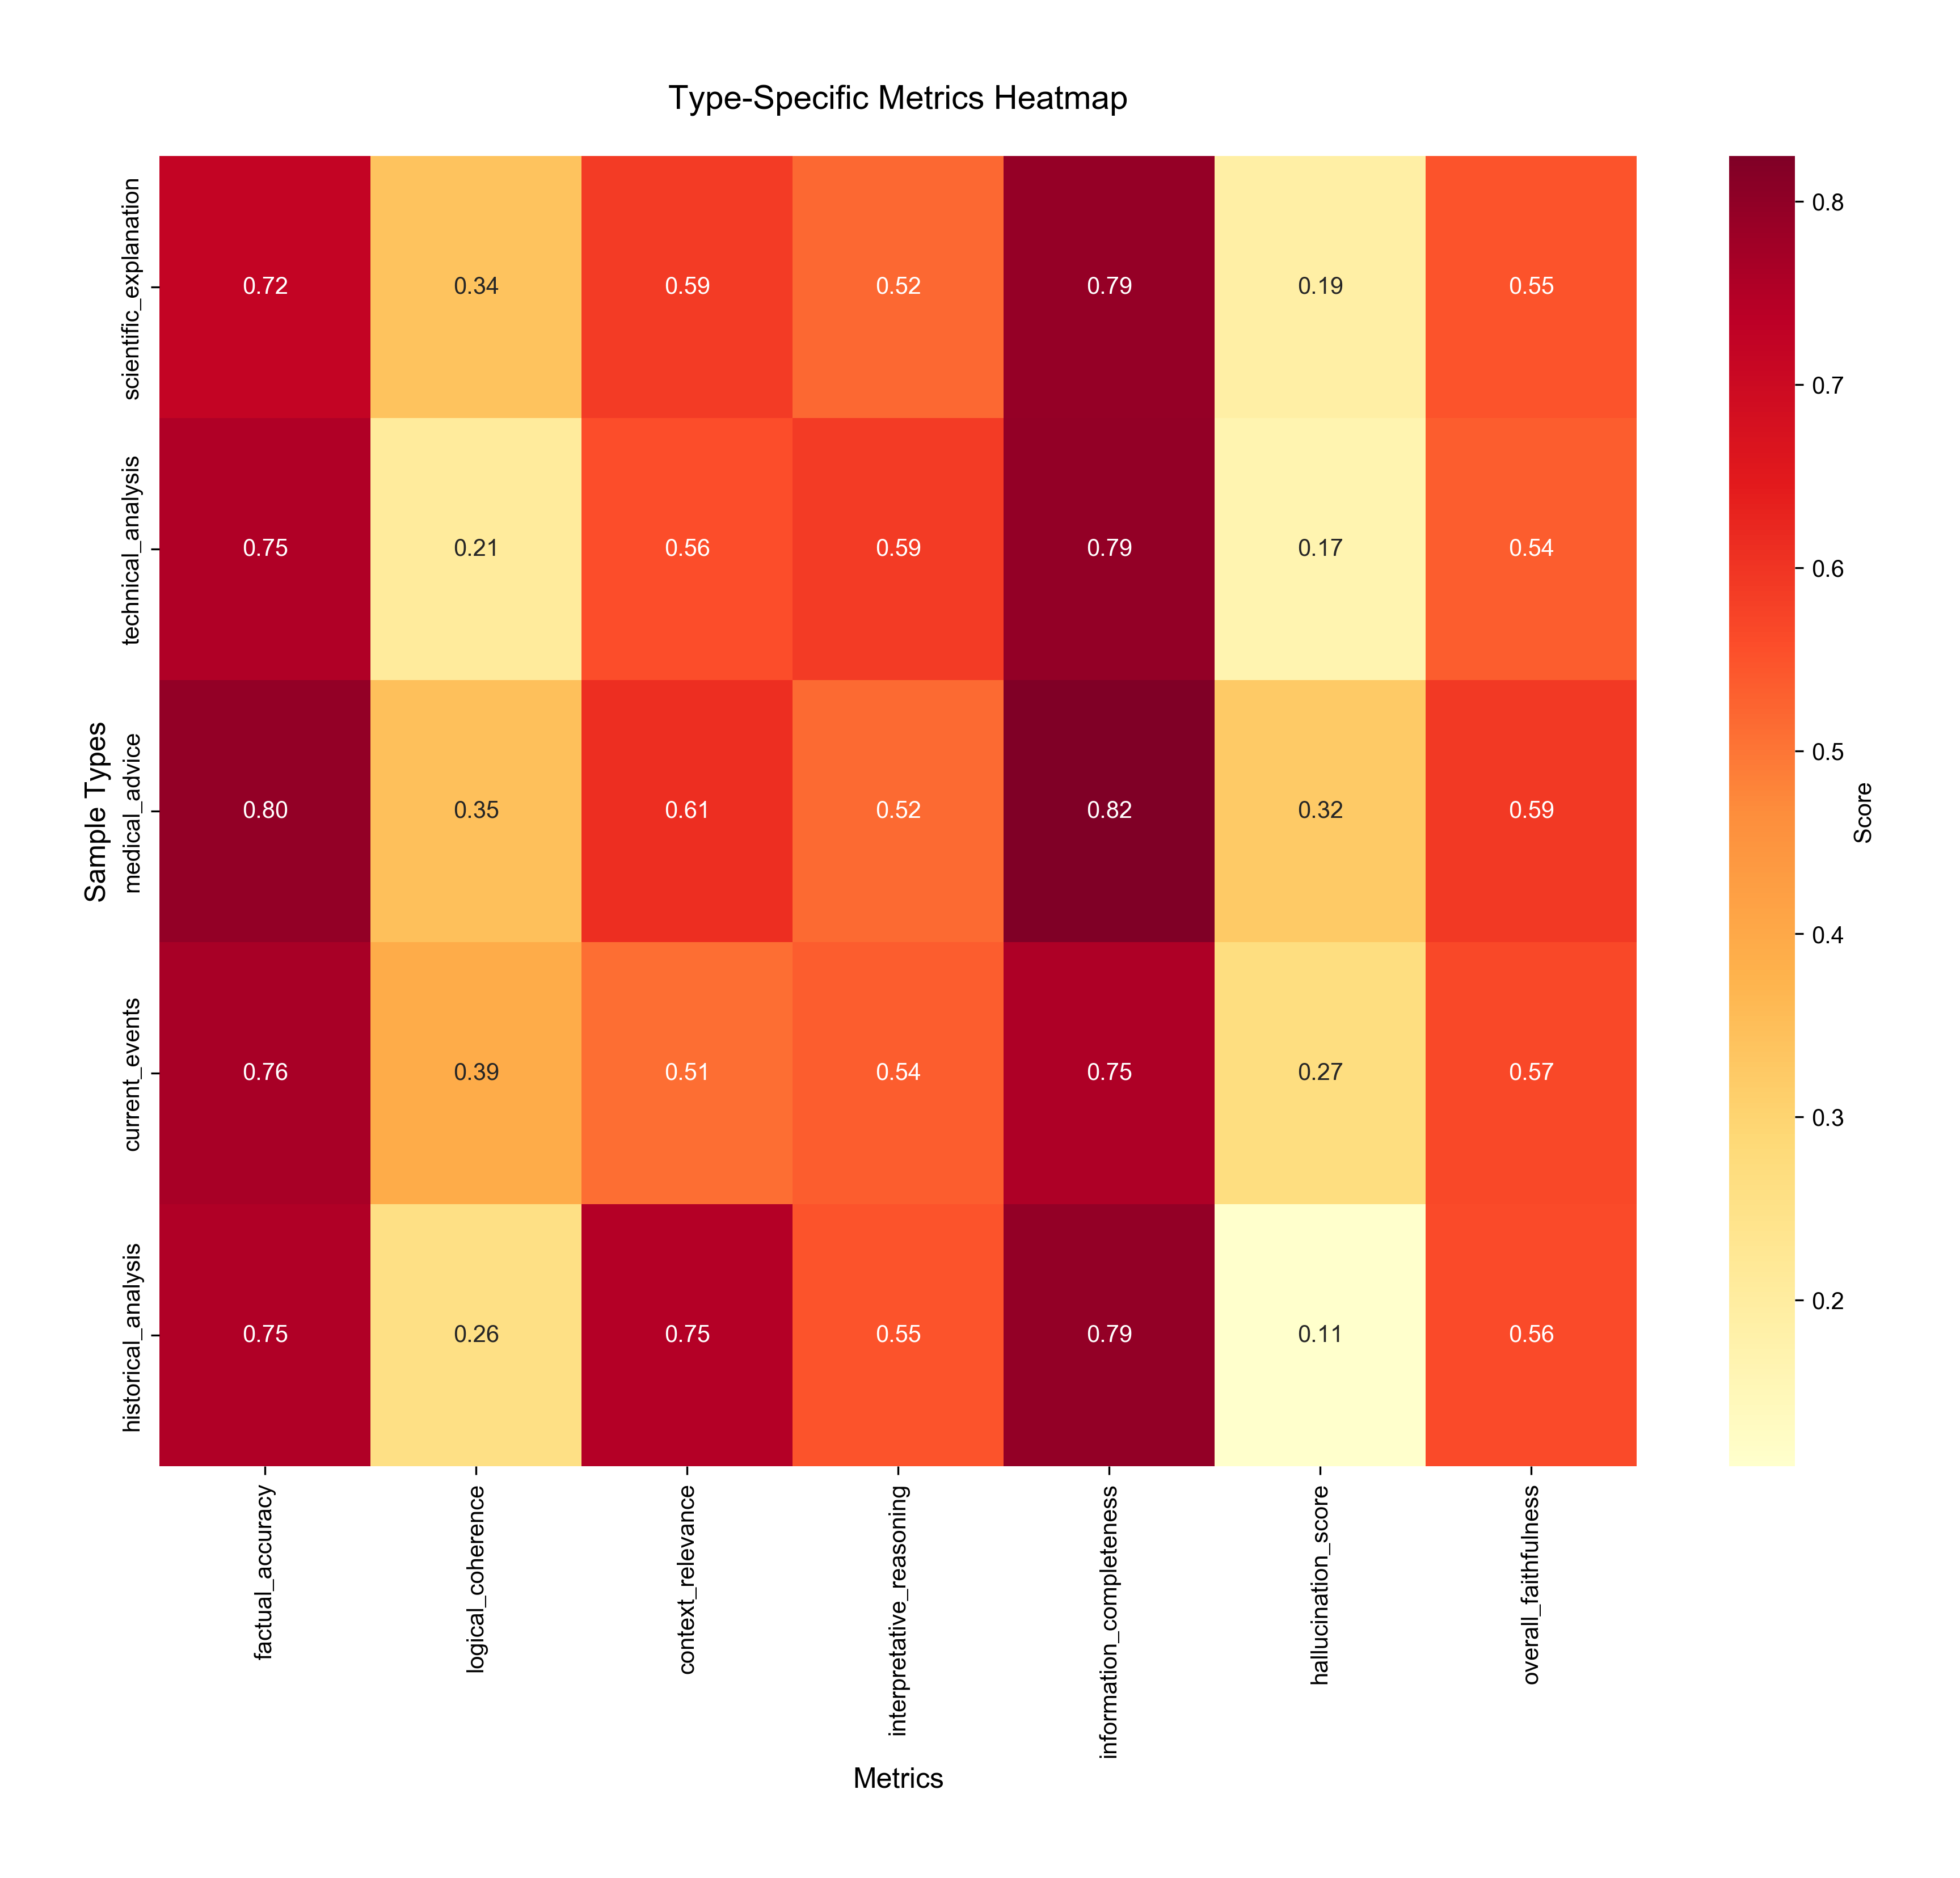
\includegraphics[width=\textwidth]{figures/visualization/metrics_heatmap_gpt-4-turbo.png}
    \caption{GPT-4-Turbo}
    \label{fig:metrics_heatmap_gpt4t}
\end{subfigure}
\hfill
\begin{subfigure}[b]{0.32\textwidth}
    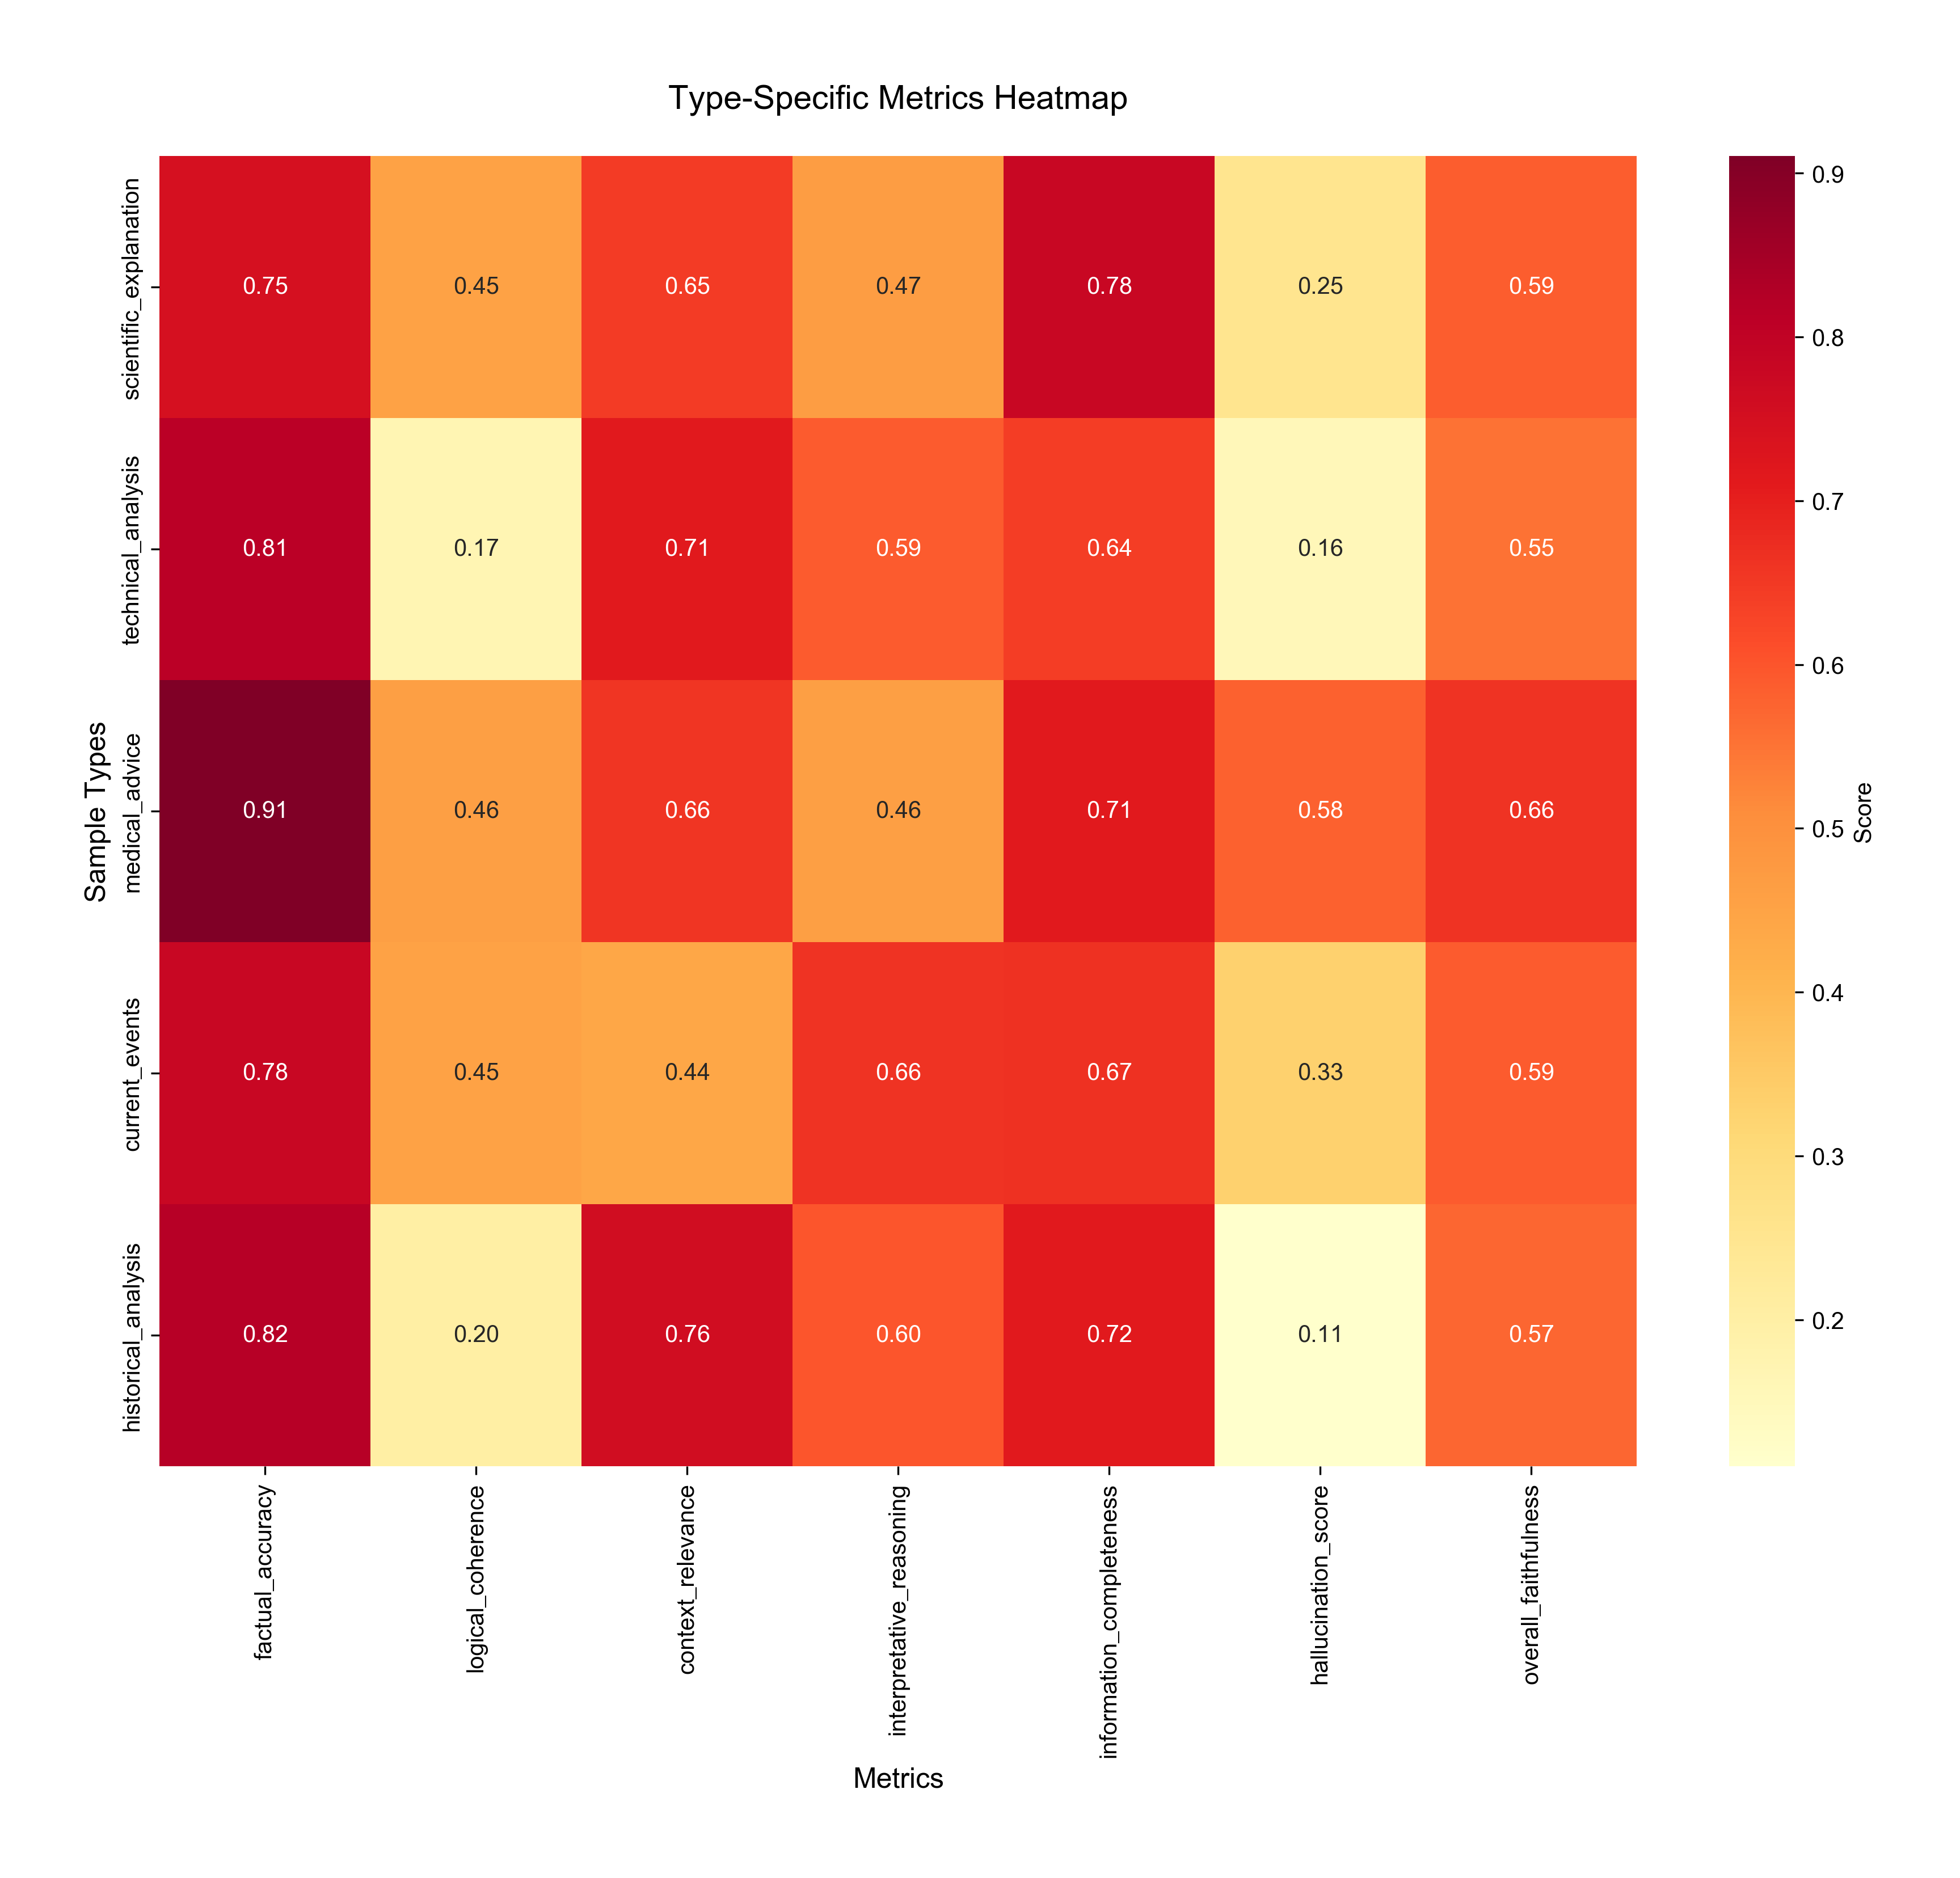
\includegraphics[width=\textwidth]{figures/visualization/metrics_heatmap_gpt-4.png}
    \caption{GPT-4}
    \label{fig:metrics_heatmap_gpt4}
\end{subfigure}
\caption{Metric Correlation Heatmaps by Model}
\label{fig:metrics_heatmaps}
\end{figure}

\textbf{Key Correlations}:
\begin{itemize}
    \item Strong positive correlation between factual accuracy and information completeness
    \item Negative correlation between hallucination scores and logical coherence
    \item Moderate correlation between context relevance and interpretative reasoning
\end{itemize}

\subsubsection{Metric Composition Analysis}
The stacked bar analysis illustrates the relative contribution of each metric to the overall faithfulness score.

\begin{figure}[!htbp]
\centering
\begin{minipage}[t]{0.32\textwidth}
    \centering
    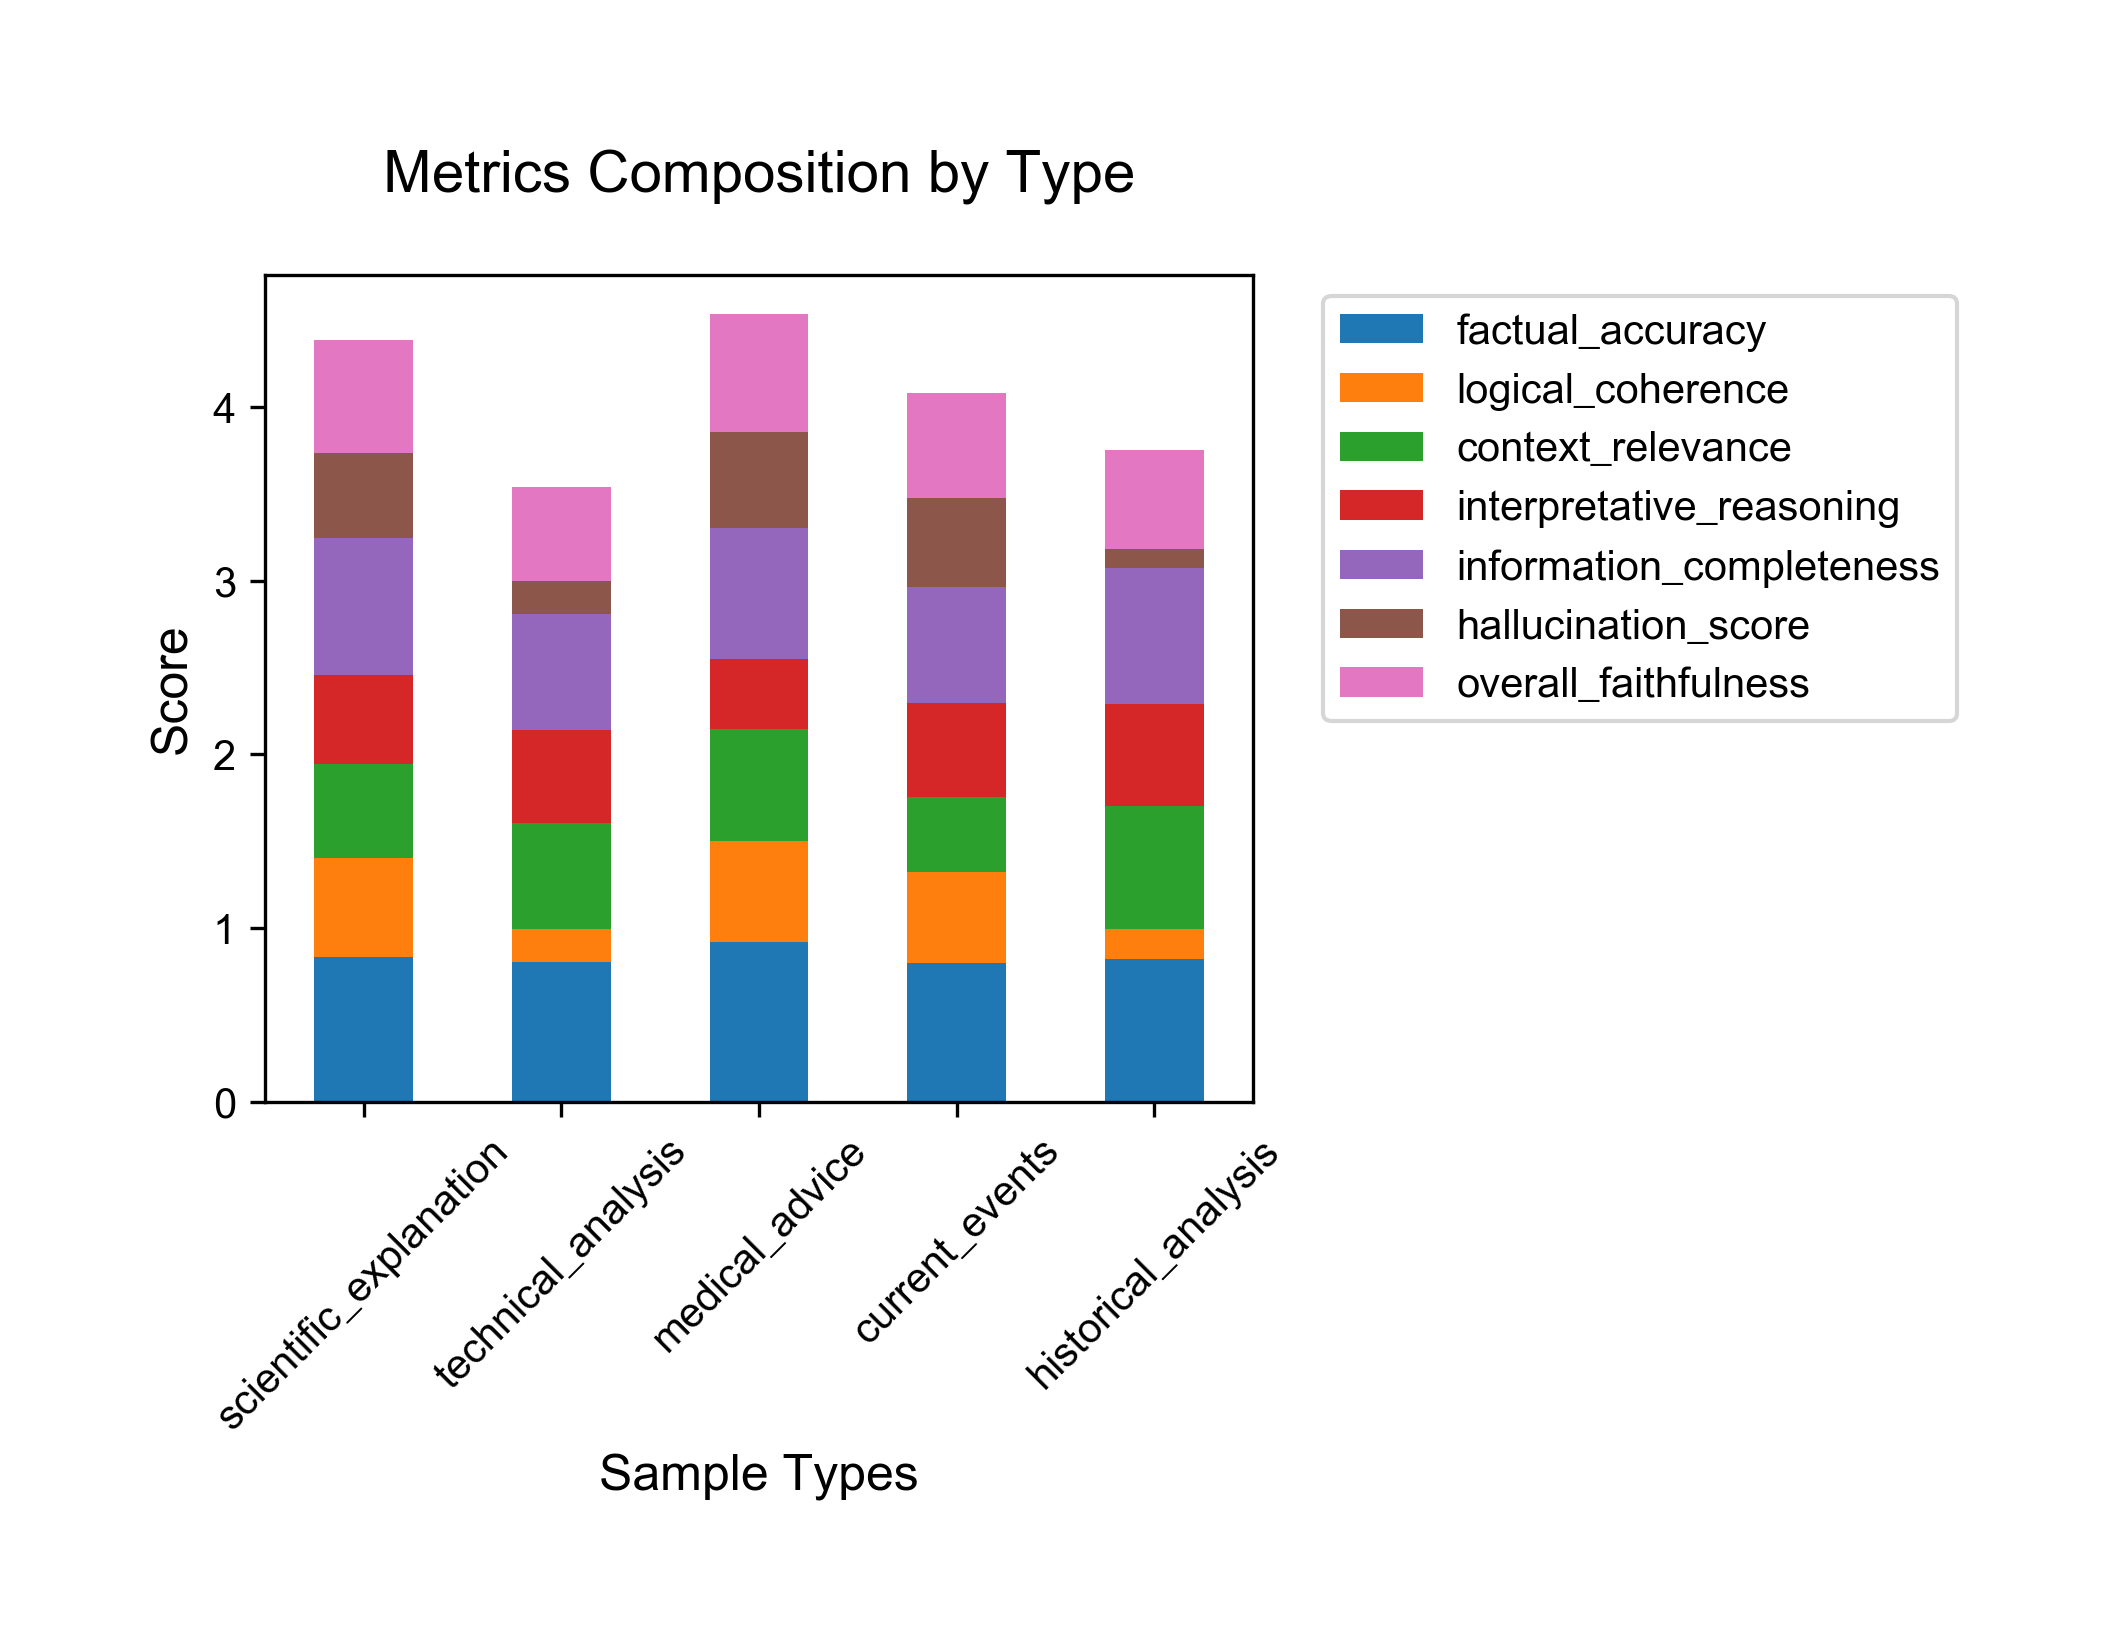
\includegraphics[width=\textwidth]{figures/visualization/metrics_stacked_bar_gpt-3.5-turbo.png}
    {\footnotesize (a) GPT-3.5-Turbo Composition}
\end{minipage}%
\begin{minipage}[t]{0.32\textwidth}
    \centering
    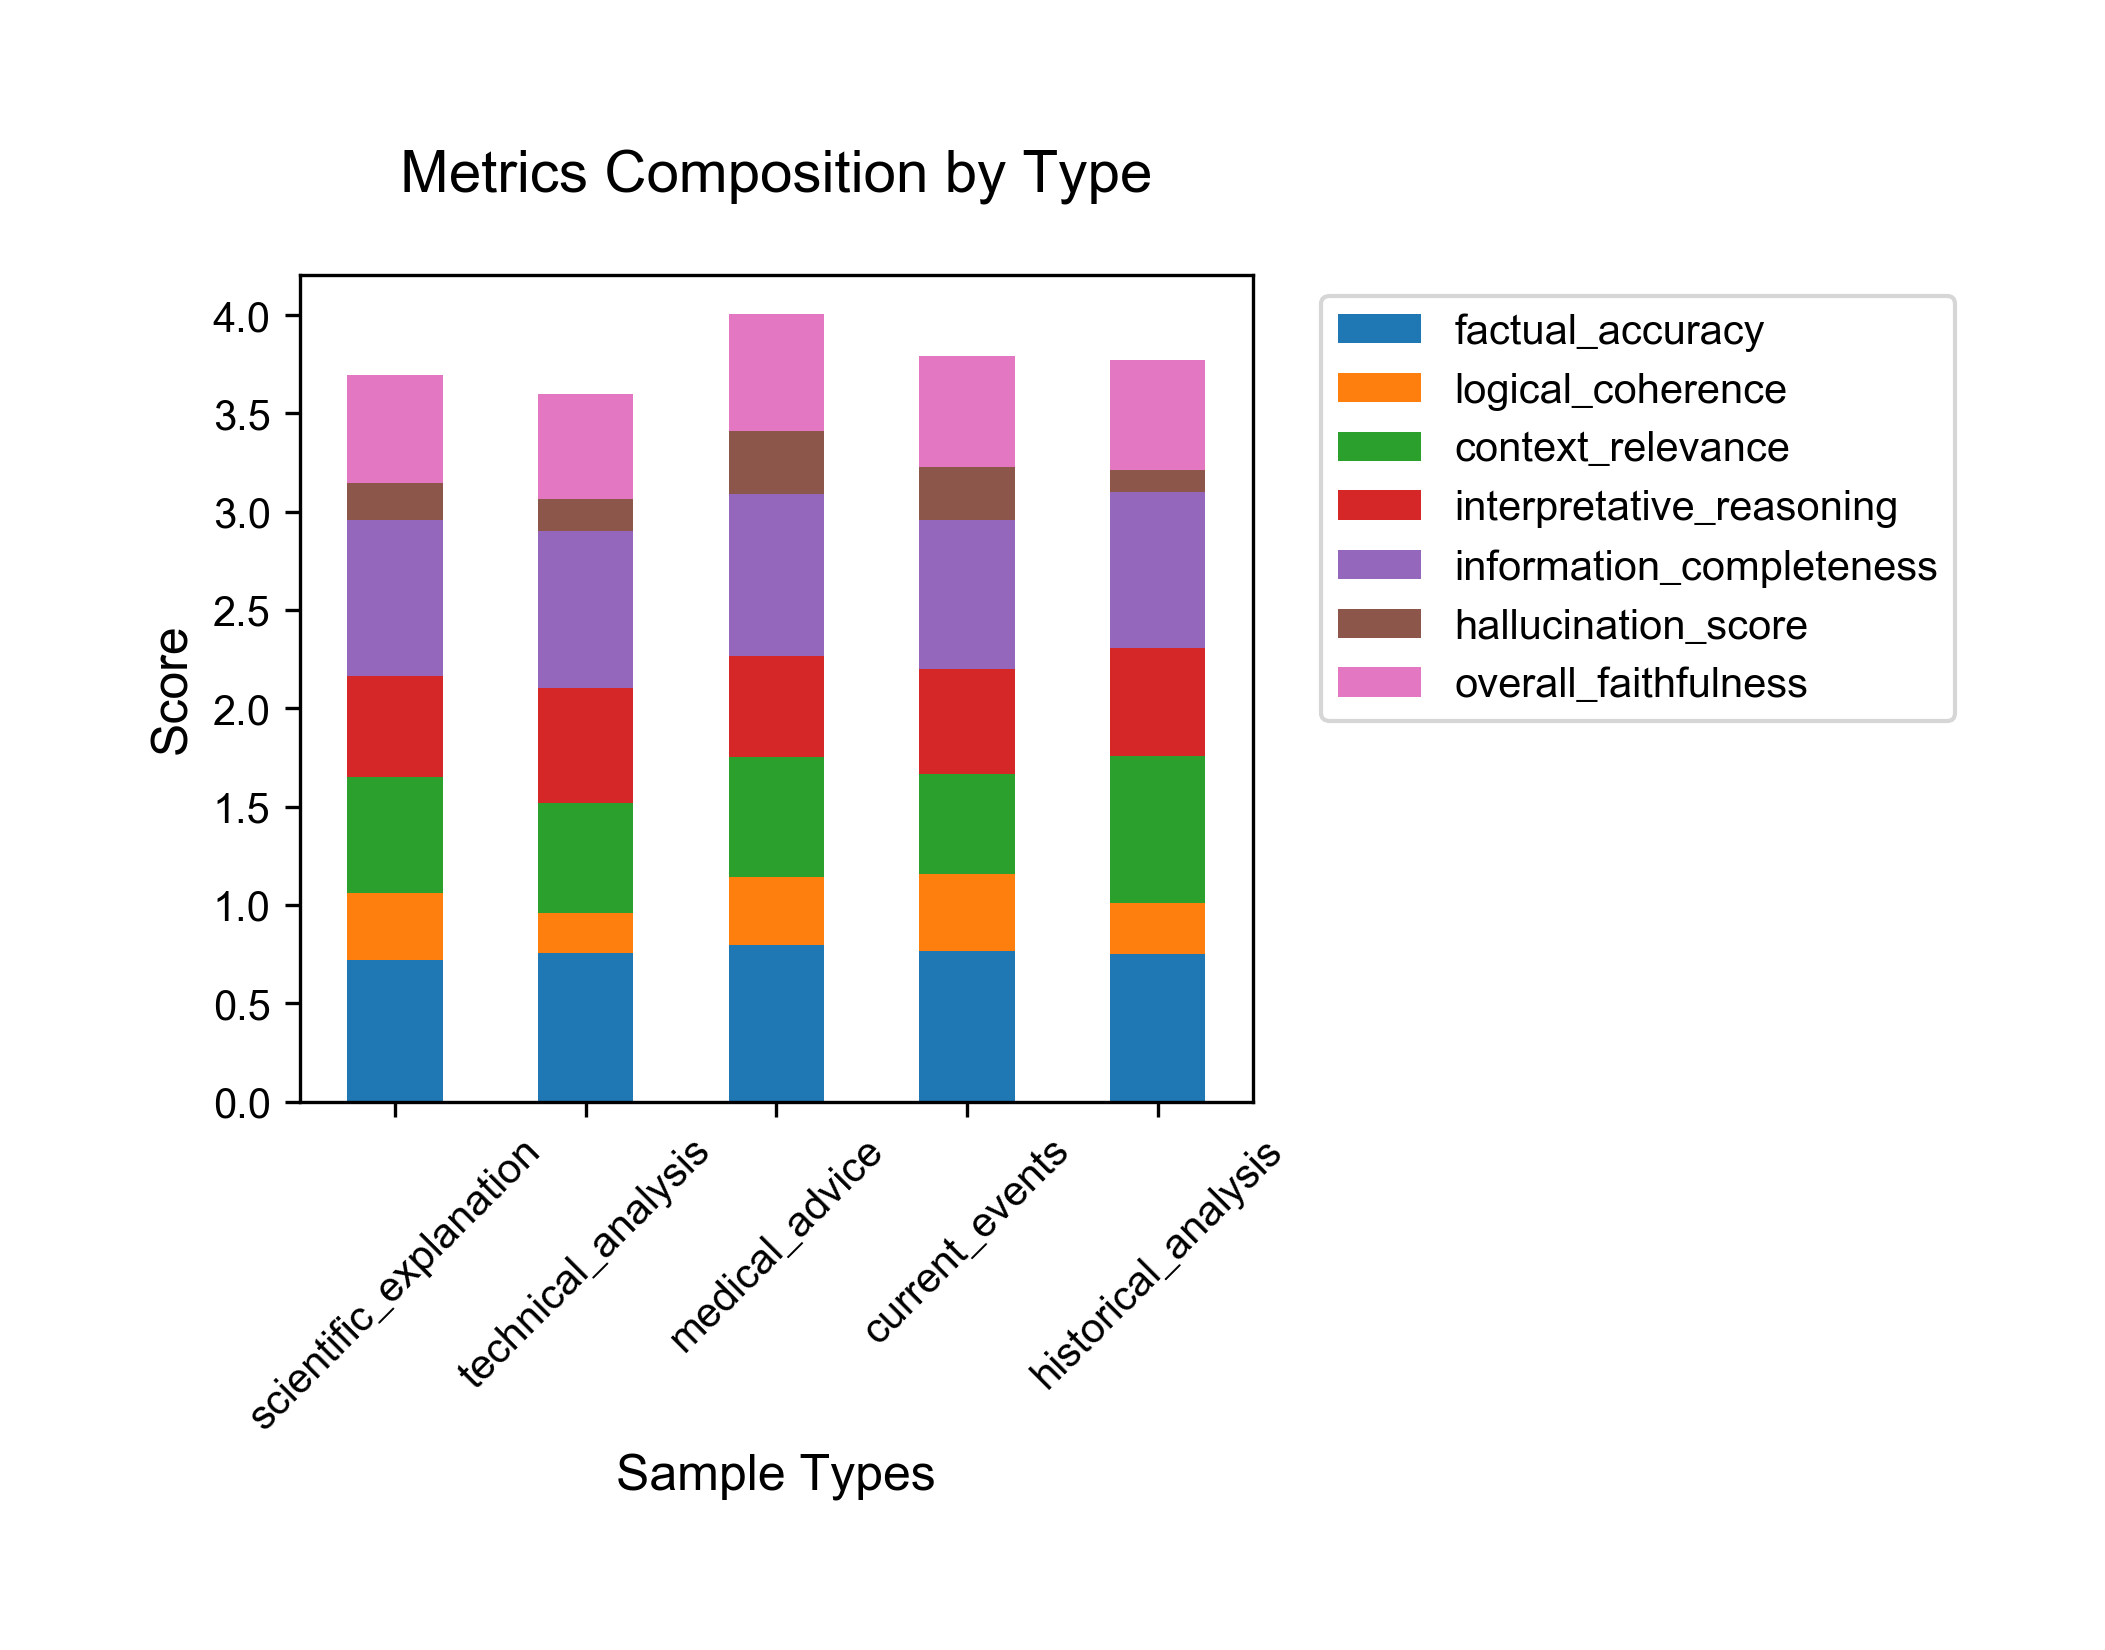
\includegraphics[width=\textwidth]{figures/visualization/metrics_stacked_bar_gpt-4-turbo.png}
    {\footnotesize (b) GPT-4-Turbo Composition}
\end{minipage}%
\begin{minipage}[t]{0.32\textwidth}
    \centering
    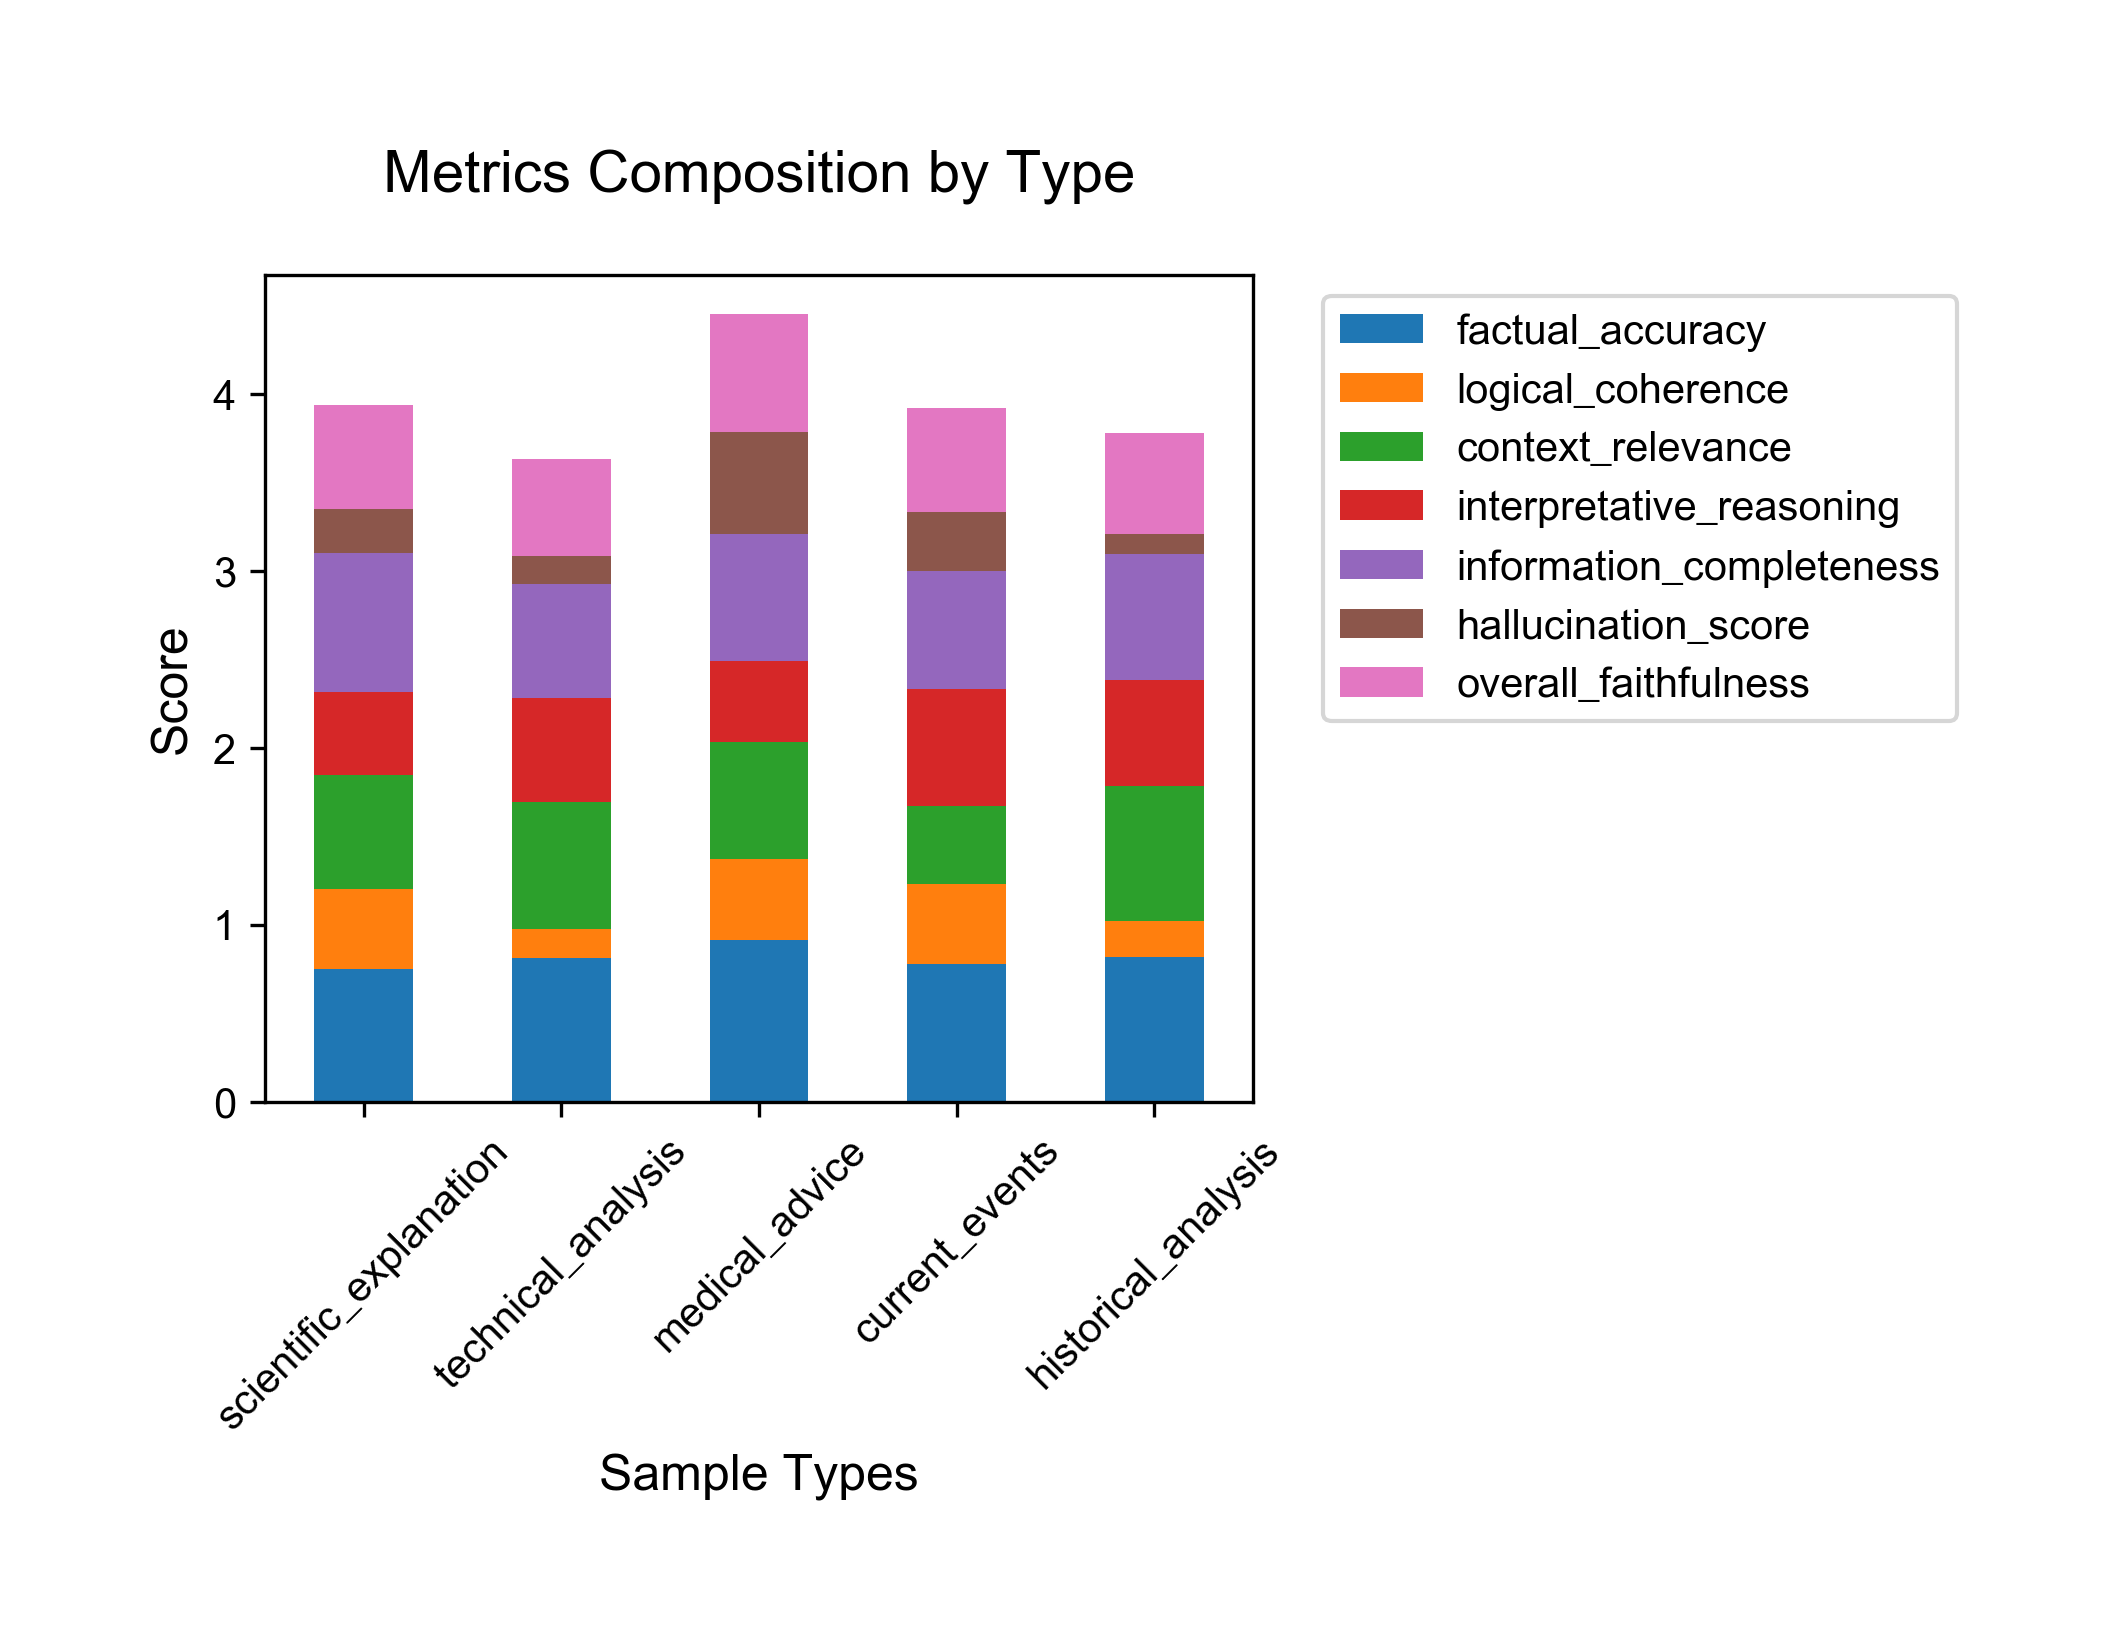
\includegraphics[width=\textwidth]{figures/visualization/metrics_stacked_bar_gpt-4.png}
    {\footnotesize (c) GPT-4 Composition}
\end{minipage}
\caption{Metric Composition Analysis by Model}
\label{fig:metrics_stacked_bars}
\end{figure}

\textbf{Composition Insights}:
\begin{itemize}
    \item Factual accuracy contributes the largest proportion to overall faithfulness
    \item Information completeness shows consistent contribution across models
    \item Hallucination scores have varying impact on different models
\end{itemize}

\subsection{Performance Patterns}
Based on our comprehensive evaluation framework described in Section 3, we identified several significant patterns in model performance.

\subsubsection{Model-Specific Patterns}
\begin{itemize}
    \item \textbf{GPT-3.5-Turbo}:
    \begin{itemize}
        \item Excels in factual accuracy (0.84) and information completeness (0.73)
        \item Shows consistent performance across different sample types
        \item Higher hallucination scores indicate potential for improvement
    \end{itemize}
    
    \item \textbf{GPT-4-Turbo}:
    \begin{itemize}
        \item Strong in information completeness (0.79) and context relevance (0.60)
        \item Lower logical coherence scores suggest areas for enhancement
        \item Most effective at minimizing hallucinations (0.21)
    \end{itemize}
    
    \item \textbf{GPT-4}:
    \begin{itemize}
        \item Balanced performance across all metrics
        \item Superior context relevance (0.64) and interpretative reasoning (0.56)
        \item Moderate hallucination control (0.29)
    \end{itemize}
\end{itemize}

\subsubsection{Type-Specific Patterns}
The analysis reveals distinct patterns across different content types, as detailed in Section~\ref{sec:evaluation}:

\begin{itemize}
    \item \textbf{Scientific Content}:
    \begin{itemize}
        \item High factual accuracy across all models (>0.75)
        \item Challenges in maintaining logical coherence
        \item Variable hallucination control
    \end{itemize}
    
    \item \textbf{Technical Content}:
    \begin{itemize}
        \item Strong context relevance (>0.60)
        \item Lower logical coherence scores (<0.40)
        \item Effective hallucination control (<0.30)
    \end{itemize}
    
    \item \textbf{Medical Content}:
    \begin{itemize}
        \item Highest factual accuracy scores (>0.80)
        \item Strong information completeness (>0.75)
        \item Variable hallucination control
    \end{itemize}
\end{itemize}

These patterns align with our initial hypotheses and provide valuable insights for future model improvements.
